
\documentclass[a4paper]{article}

\usepackage[utf8]{inputenc}   % LaTeX, comprends les accents !
\usepackage[T1]{fontenc}      % Police contenant les caractères français
\usepackage{geometry}         % Définir les marges
\usepackage[francais]{babel}  % Placez ici une liste de langues, la
                              % dernière étant la langue principale
\usepackage{graphicx}         % Inserer des images
\usepackage{gensymb}
\usepackage{color}

\pagestyle{headings}          % Pour mettre des entêtes avec les titres
                              % des sections en haut de page

\title{\bf The NIKA data analysis pipeline}           % Les paramètres du titre : titre, auteur, date
\author{{\it The NIKA collaboration}}
\date{\today}

\setlength{\textwidth}{15.5cm}
\setlength{\textheight}{23cm}
\oddsidemargin +0.5cm                                          % Marges
\evensidemargin +0.5cm
\topmargin +0cm

\begin{document}

\maketitle                    % Faire un titre utilisant les données
                              % passées à \title, \author et \date
\begin{figure}[!h]
\centering

\includegraphics[height=2cm,trim=0cm 0.1cm 0.1cm 0.1cm, clip=true]{Figure/nika_white_bg}
\end{figure}
\vspace*{0.5cm}

\setcounter{page}{1}
\setcounter{tocdepth}{1}

%______________________________________________________________________________
%\section*{Abstract}
%\label{sec:abstract}
%\input{000_abstract}
%%______________________________________________________________________________
%\section{Introduction}
%\label{sec:introduction}
%\input{010_introduction}
%%______________________________________________________________________________
%\section{Real time}
%\label{sec:real_time}
%\input{020_real_time}
%%______________________________________________________________________________
%\section{Focal plane reconstruction}
%\label{sec:focal_plane}
%\input{030_focal_plane}
%%______________________________________________________________________________
%\section{Calibration}
%\label{sec:calibration}
%\input{040_calibration}
%%______________________________________________________________________________
%\section{Data selection}
%\label{sec:data_selection}
%\input{050_data_slection}
%%______________________________________________________________________________
%\section{Decorrelation}
%\label{sec:decorrelation}
%\input{060_decorrelation}
%%______________________________________________________________________________
%\section{Fourier filtering}
%\label{sec:fourier_filtering}
%\input{070_fourier_filtering}
%%______________________________________________________________________________
%\section{Mapmaking}
%\label{sec:mapmaking}
%\input{080_mapmaking}
%%______________________________________________________________________________
%\section{Noise estimations}
%\label{sec:noise_measurement}
%\input{090_noise_measurement}
%%______________________________________________________________________________
%\section{Simulations}
%\label{sec:simulation}
%\input{100_simulation}
%%______________________________________________________________________________
%\section{Conclusions}
%\label{sec:conclusion}
%\input{110_conclusion}




%%%%%%%%%%%%%%%
\section{Introduction}
This note gives an overview of the {\it NIKA} pipeline as it is during the Run6. Sect.~\ref{sec:example} starts by describing the case of an example script (M87) that can be use without the complete knowledge of the modules content. It shows how to use the pipeline and what are the outputs. The parameters of the pipeline are described in Sect.~\ref{sec:param}. In Sect.~\ref{sec:module_description}, we describe the content of each module and the way to implement new modules ({\it i.e.} decorrelation methods, filtering). Finally, Sect.~\ref{sec:simu} describes the simulation pipeline in the case of flux Time Ordered Data (TOD) only and in the case of the full simulation of the {\it NIKA} camera, including the simulation of the transmission line with its resonances and the $I$, $Q$, $dI$, $dQ$ TODs for each tone.

%%%%%%%%%%%%%%%
\section{How to use it -- quick start and example script}
\label{sec:example}
\subsection{Aims of the scripts}
An example script can be found under {\color{blue} your\_SVN\_path/Pipeline/Run6/Scr/example\_v1.pro}. It uses the 8 scans of M87 taken during the Run5. A similar file should be created for each source that you want to reduce with the pipeline. The aim of such file is to define the scans which should be used, to set the appropriate parameters, and to launch the pipeline. The final output are the maps of flux, variance and time per pixel at both wavelength, with the proper astrometry. In the case of the example script, we also briefly analyze the outputs of the pipeline and plot some results.

\subsection{Information to be given by hand}
\label{sec:info_hand}
First, the users have to specify informations that cannot be guessed by the pipeline.
\begin{itemize}
\item The name of the source, here \\
{\color{blue} source = 'M87'}
\item The version of the reduction in case you want to compare different analysis, such as \\
{\color{blue} version = 'v1'}
\item The name used for the saved files. In this example it is set identical to the name of the source with empty spaces replace by underscores, so in fact it is also M87 since there are no empty spaces\\
{\color{blue} name4file = STRJOIN(STRSPLIT(source, /EXTRACT), '\_')}
\item The pointing coordinates and the source coordinates in R.A -- Dec, given in a structure. Only the difference between the two matters in the reduction but the saved astrometry requires the right coordinates. In the case of this example, they are both the same: \\
{\color{blue} coord\_\{pointing, source\} = \{ra:[12.0,30.0,49.40], dec:[+12.0,23.0,28.0]\}}
\item The scans used with the corresponding days. In the case of this example we have \\
{\color{blue} scan\_num = [104, 105, 107, 108, 109, 110, 112, 113]}\\
{\color{blue} day = '201211'+['24', '24', '24', '24', '24', '24', '24', '24']}
\item The output directory where the saved file should go. If it does not exist then it is created. Hhere we have \\
{\color{blue} output\_dir = !nika.save\_dir+"/Example\_script"}
\end{itemize}

\subsection{Init the parameters}
The script inits a default parameter structure which uses the given scans ({\color{blue} nika\_pipe\_default\_param, scan\_num, day, param}). The content of this structure is described in details in Sect.~\ref{sec:param}, but as a start, the user who does not know what the parameters correspond to can leave most of them as they are, by default. Only the parameters given by hand have to be changed as it is done in the example script:\\
{\color{blue} param.source = source\\
param.name4file = name4file\\
param.version = version\\
param.coord\_pointing = coord\_pointing\\
param.coord\_source = coord\_source\\
param.output\_dir = output\_dir\\
param.decor.method = 'COMMON\_MODE\_KIDS\_FAR'\\
param.map.reso = 2\\
param.map.size\_ra = 300\\
param.map.size\_dec = 300}\\
Note that here we also change the decorrelation method, the resolution and the size of the product map; but it is not mandatory.

\subsection{The launch of the pipeline}
After having saved the parameter file under the name param followed by the filename and its version in the output directory, such as 
{\color{blue} output\_directory/param\_M87\_v1.save} here, the analysis starts with {\color{blue} nika\_pipe\_launch, param, map\_combi, map\_list, /save, /map\_per\_kid, /ps}. The outputs are the combined maps and the maps per scan structures. Their contents are described, as well as the keywords, in Sect.~\ref{sec:nika_pipe_launch}.

\subsection{Brief analysis example}
This section describes the results of a brief analysis made in the example script so that the user can check that the pipeline produce consistent results, by writing the same files as those shown here in the defined output directory. During the pipeline, intermediate result files have been saved in the output directory and are first recovered. 

The maps per scans that are produced are shown for both wavelength with the associated combined maps on Fig.~\ref{fig:M87_map_per_scan}.
\begin{figure}
\centering
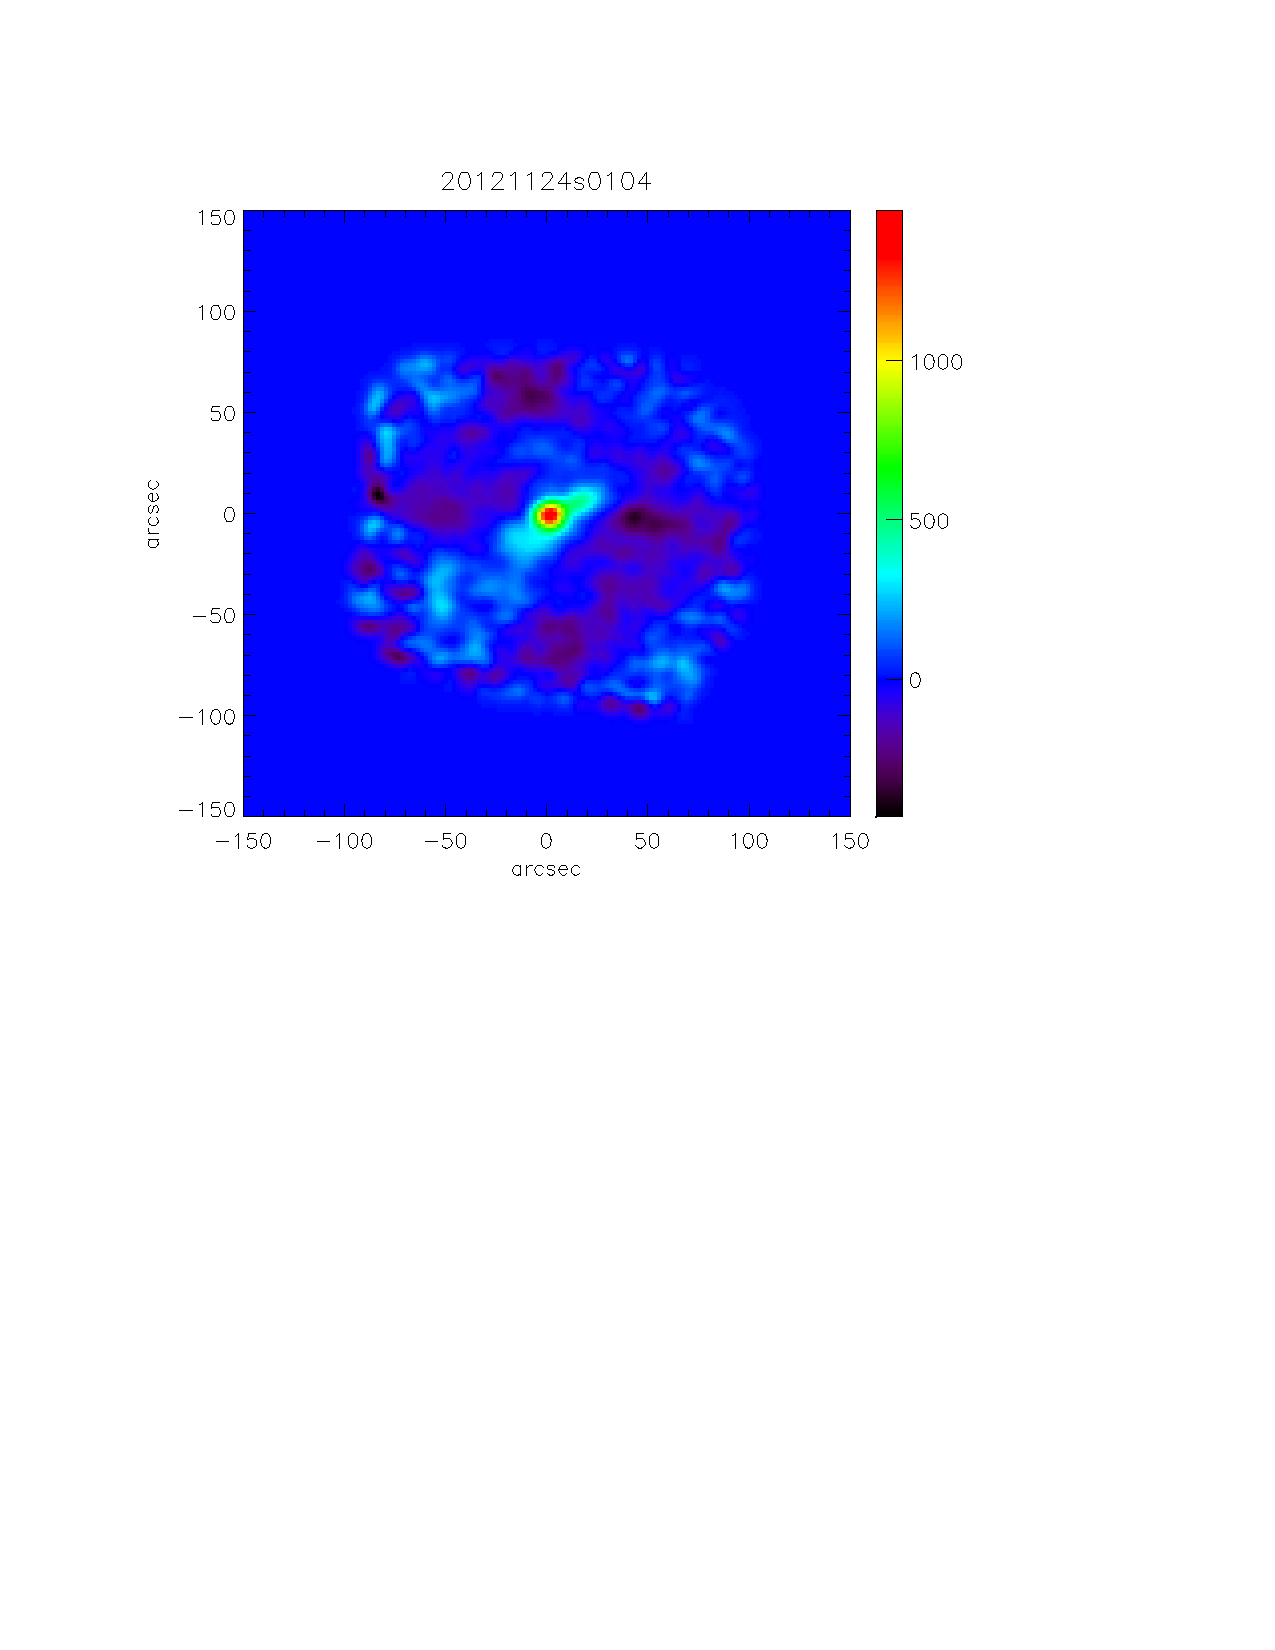
\includegraphics[height=3cm, trim=2cm 13cm 4cm 2cm, clip=true]{Figure/map_1mm_scan20121124s0104}
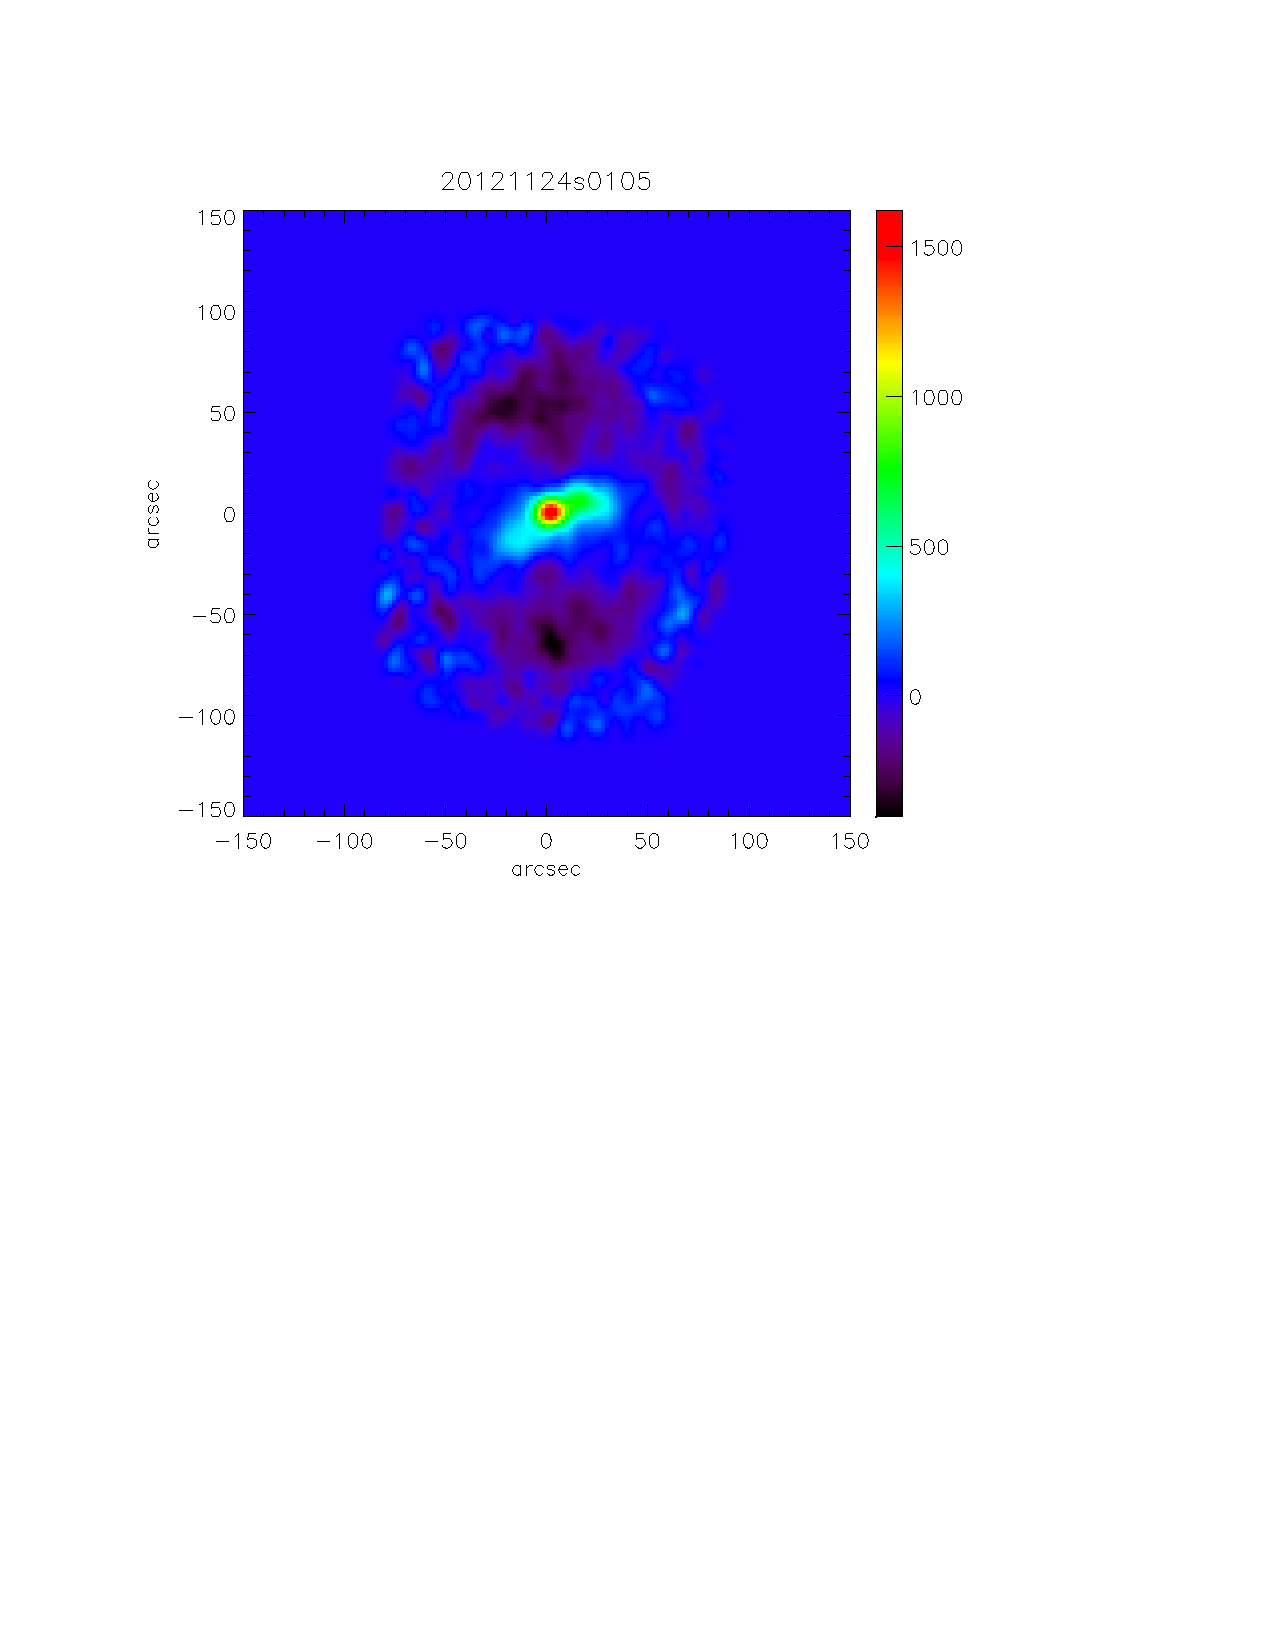
\includegraphics[height=3cm, trim=2cm 13cm 4cm 2cm, clip=true]{Figure/map_1mm_scan20121124s0105}
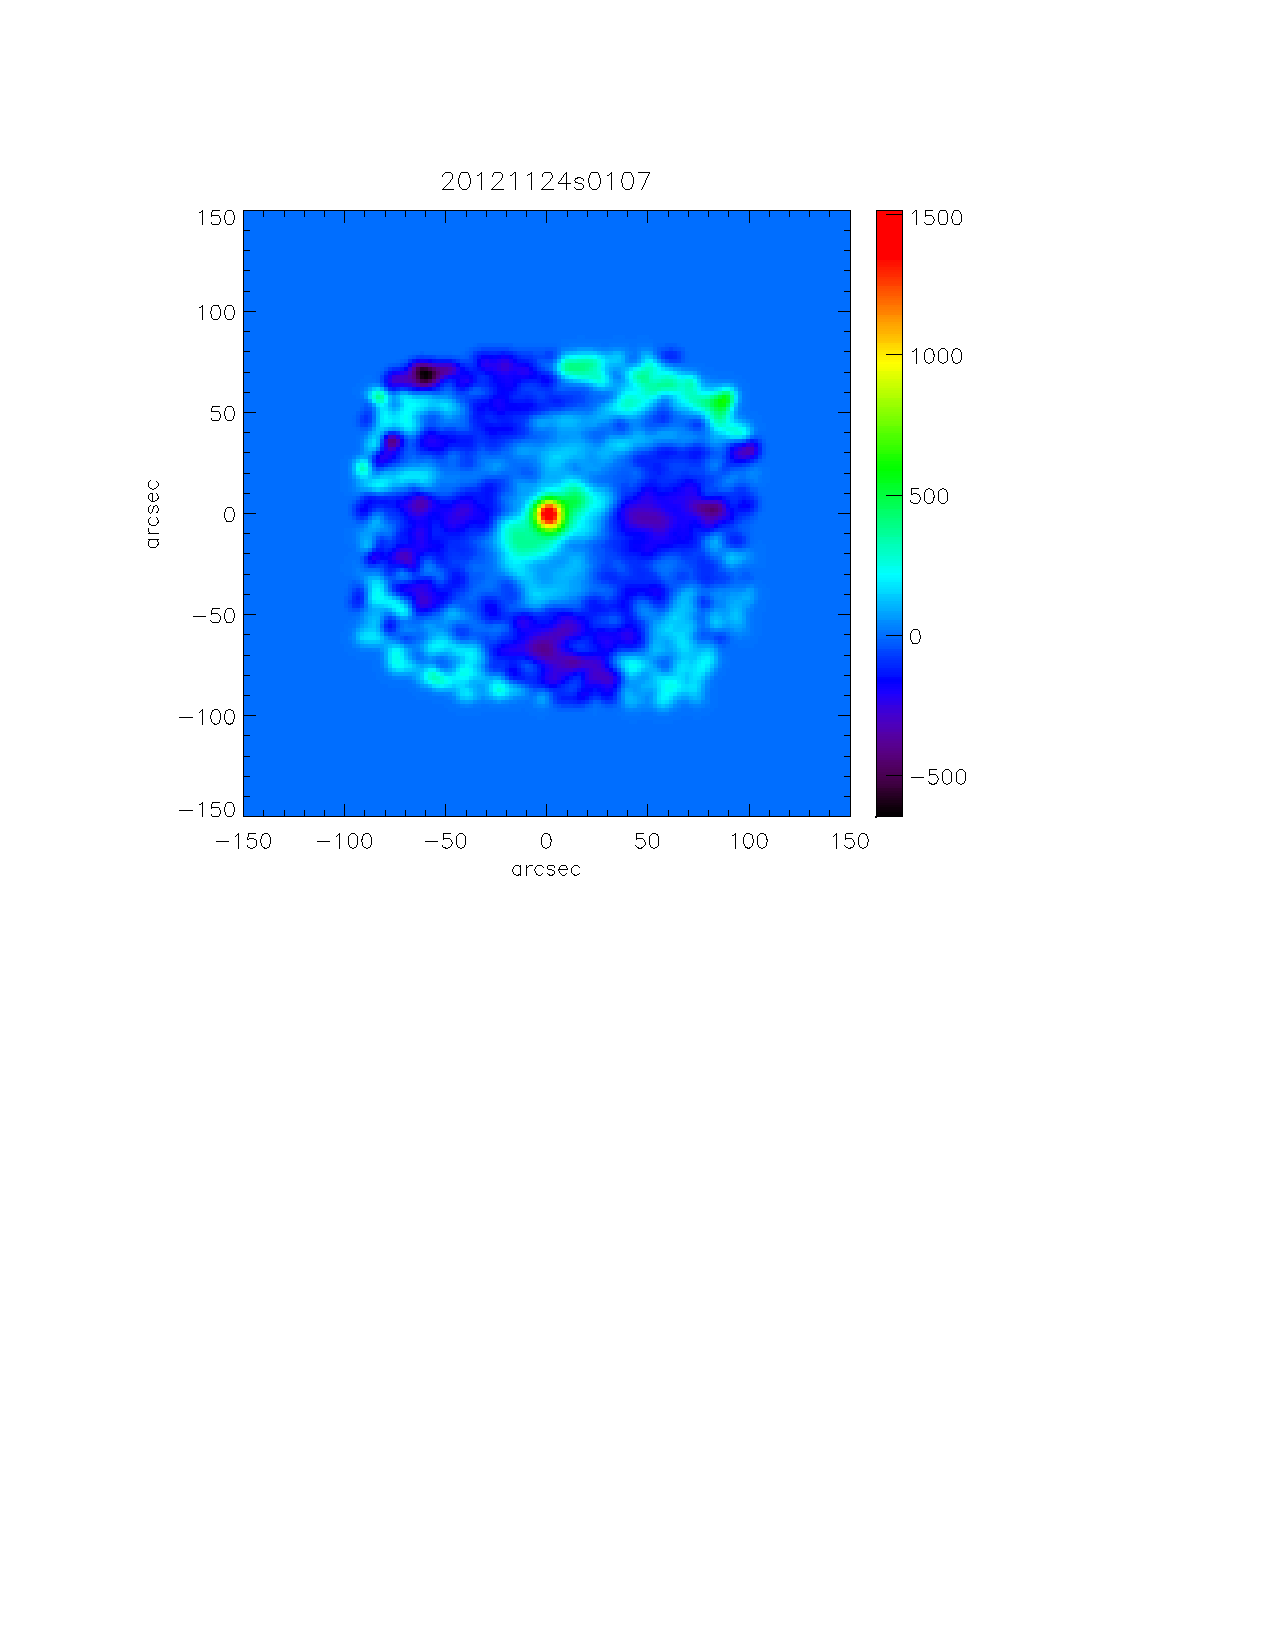
\includegraphics[height=3cm, trim=2cm 13cm 4cm 2cm, clip=true]{Figure/map_1mm_scan20121124s0107}
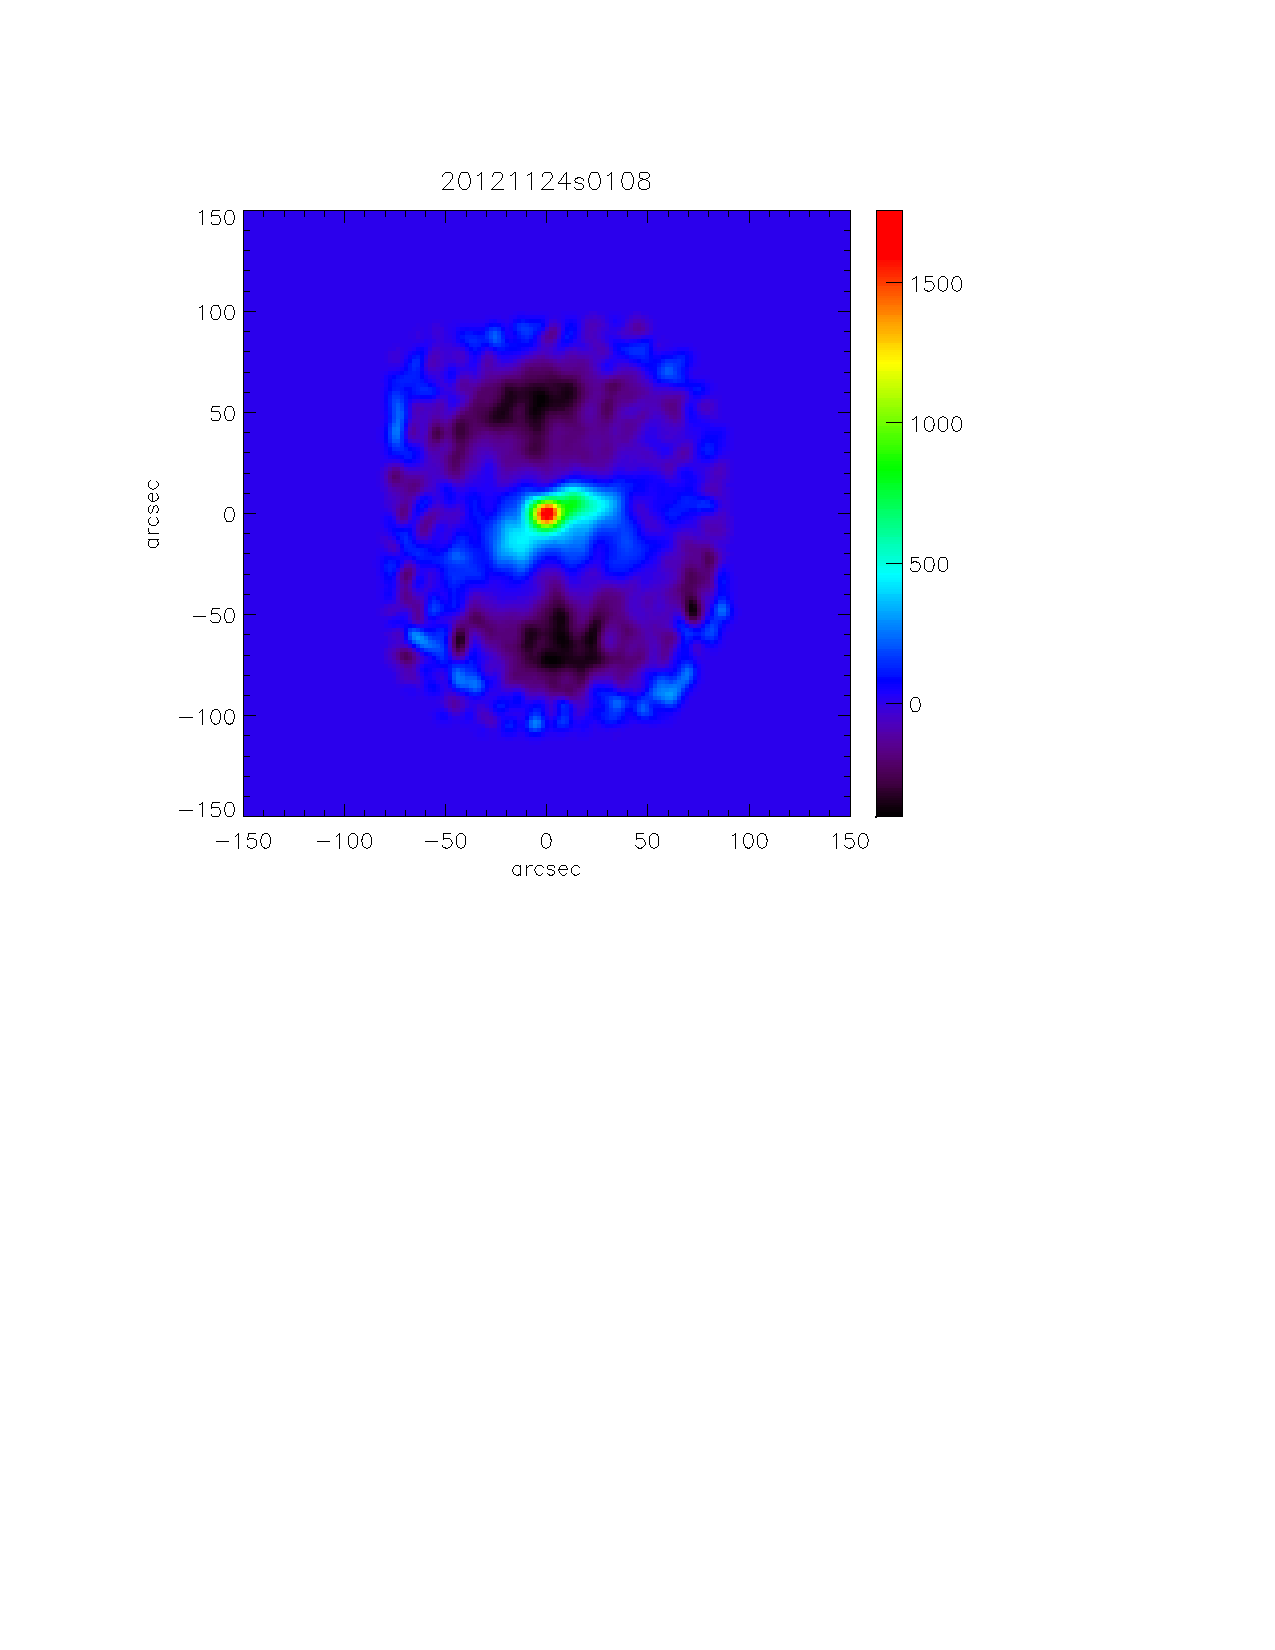
\includegraphics[height=3cm, trim=2cm 13cm 4cm 2cm, clip=true]{Figure/map_1mm_scan20121124s0108}
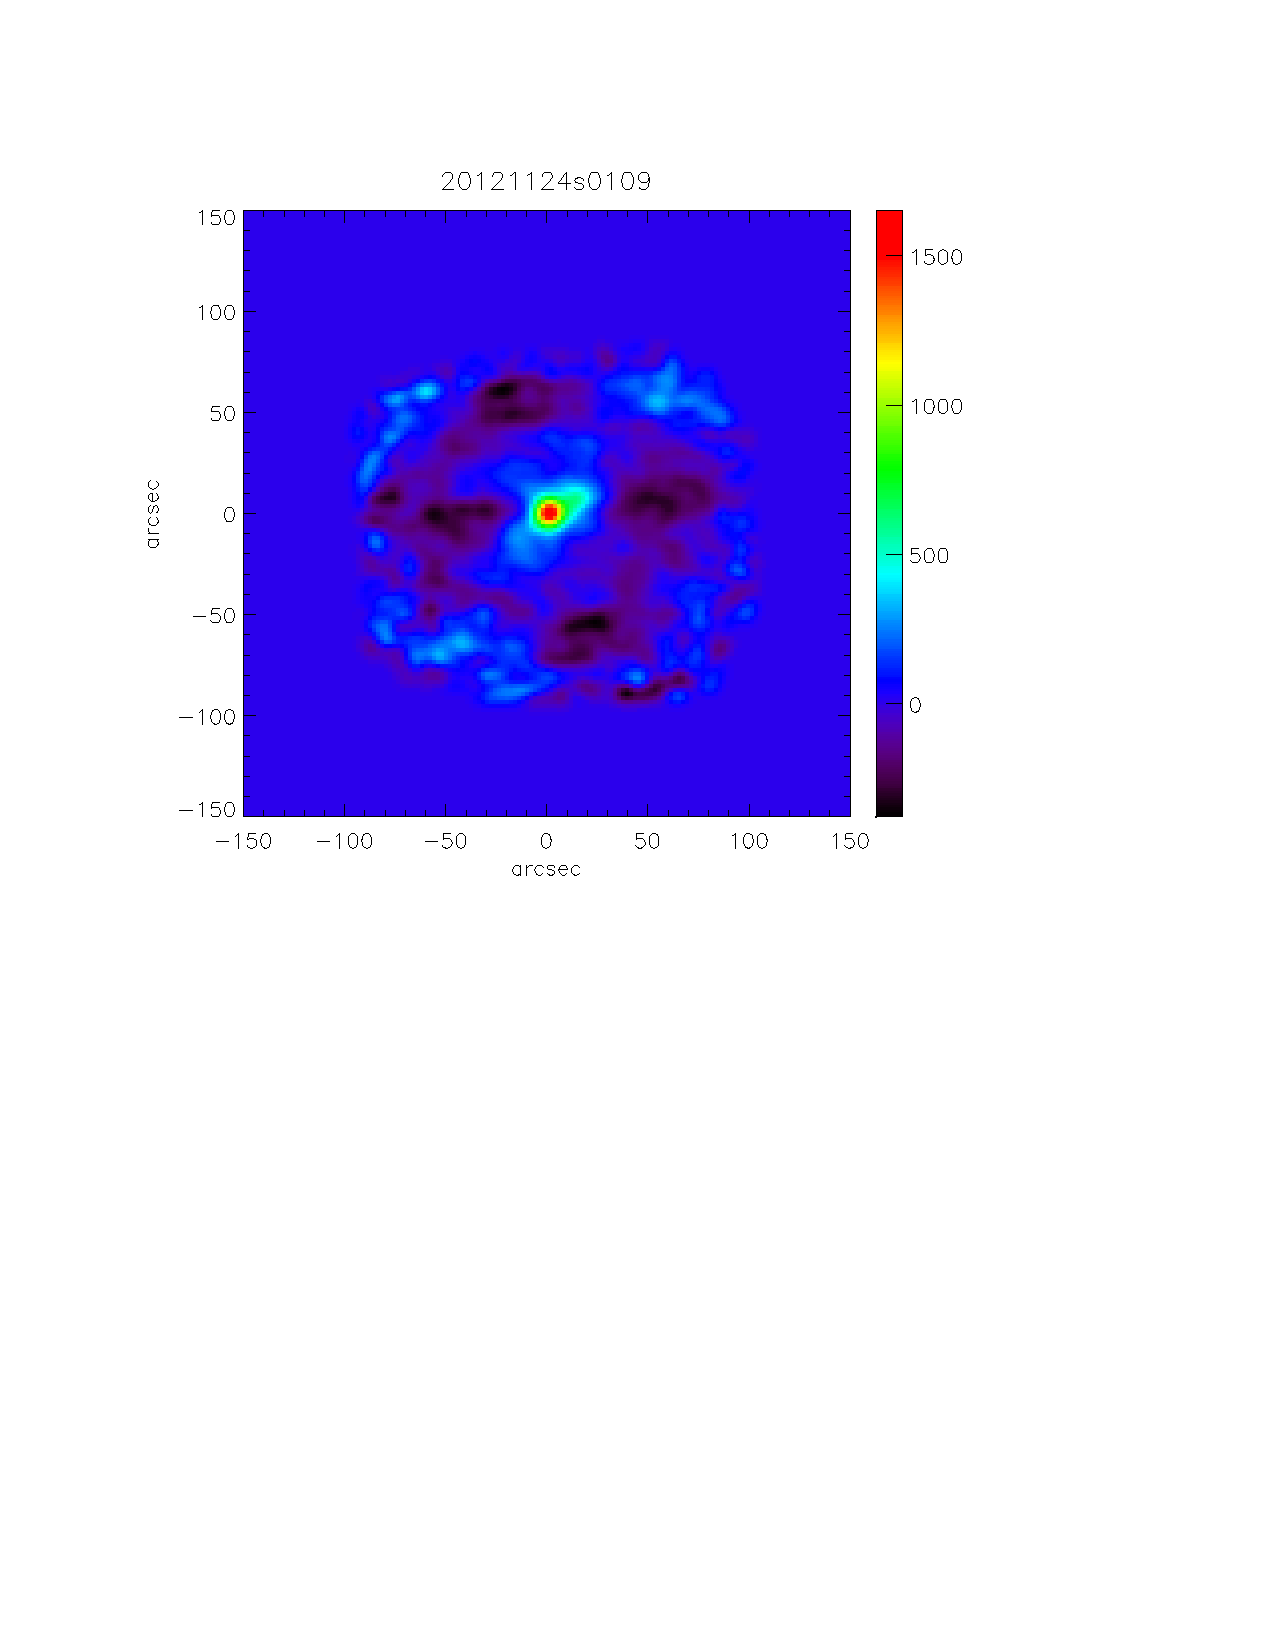
\includegraphics[height=3cm, trim=2cm 13cm 4cm 2cm, clip=true]{Figure/map_1mm_scan20121124s0109}
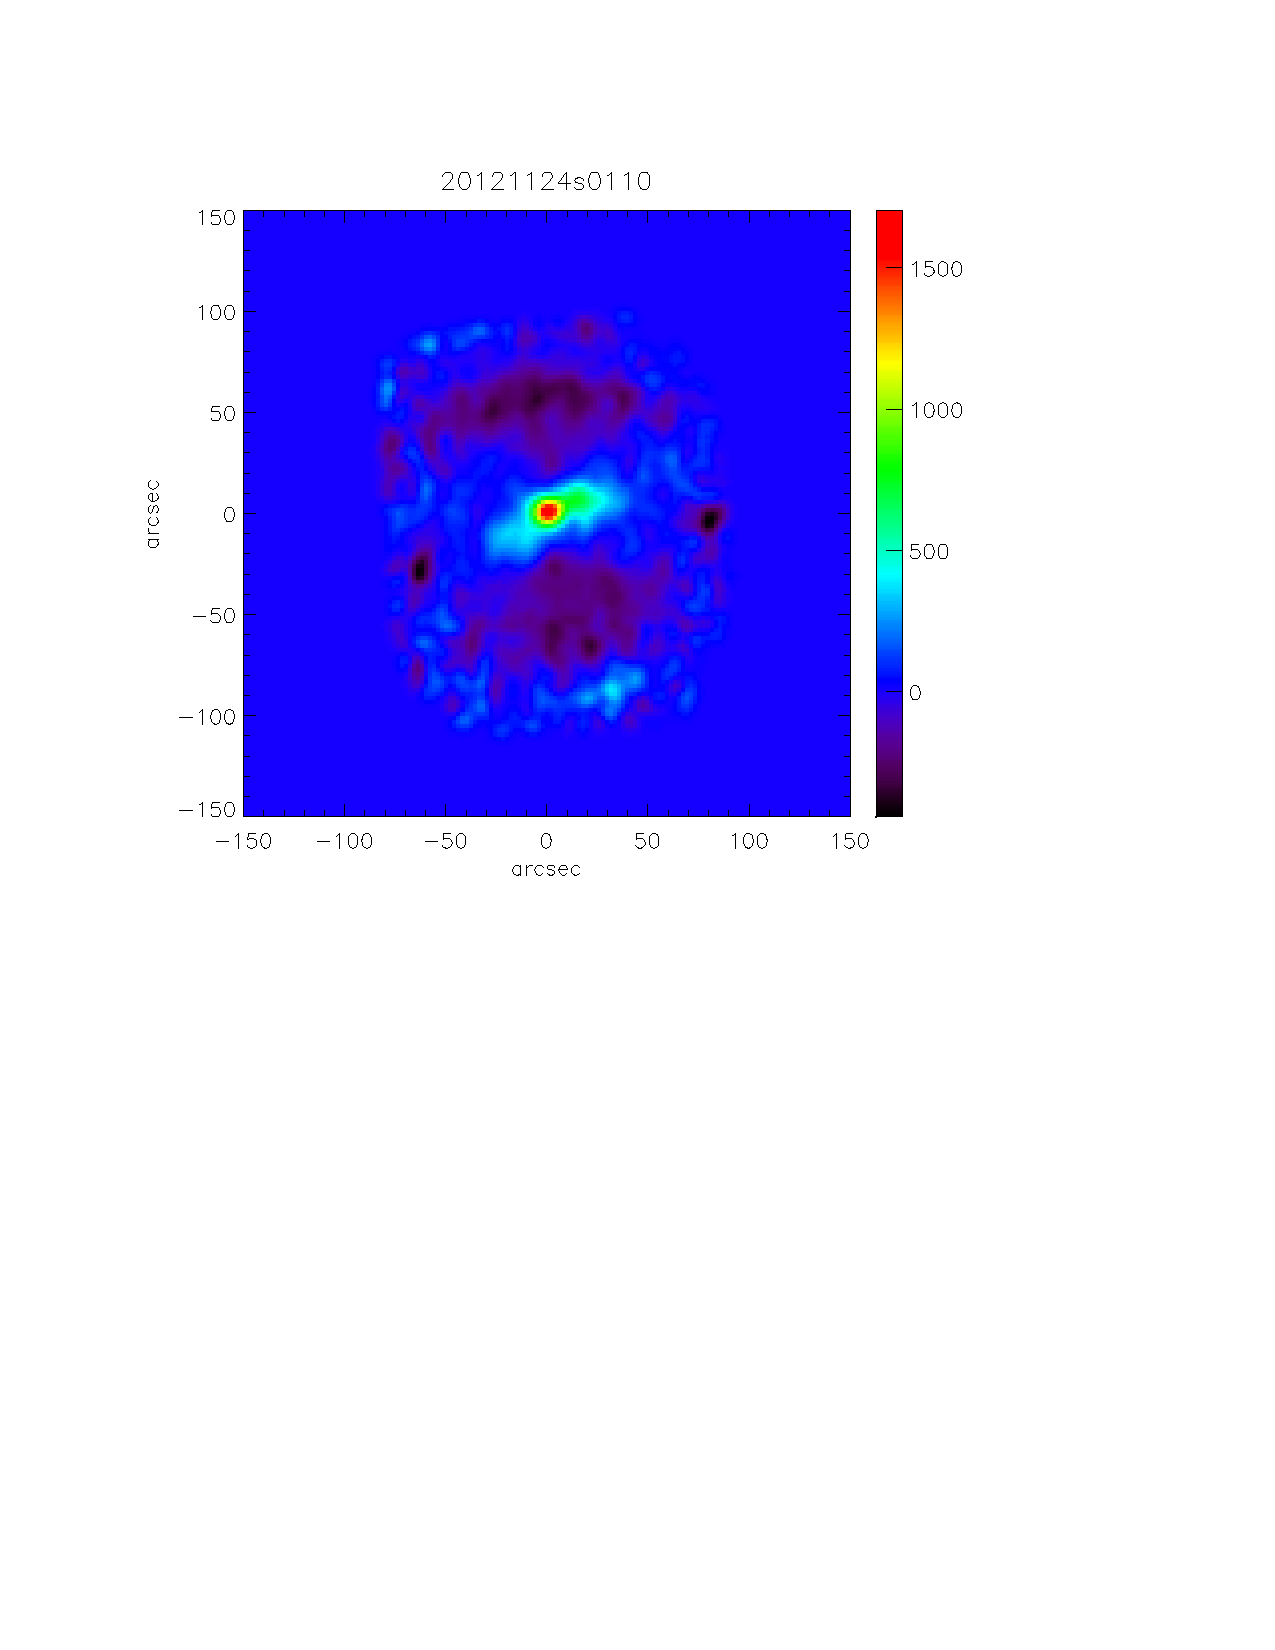
\includegraphics[height=3cm, trim=2cm 13cm 4cm 2cm, clip=true]{Figure/map_1mm_scan20121124s0110}
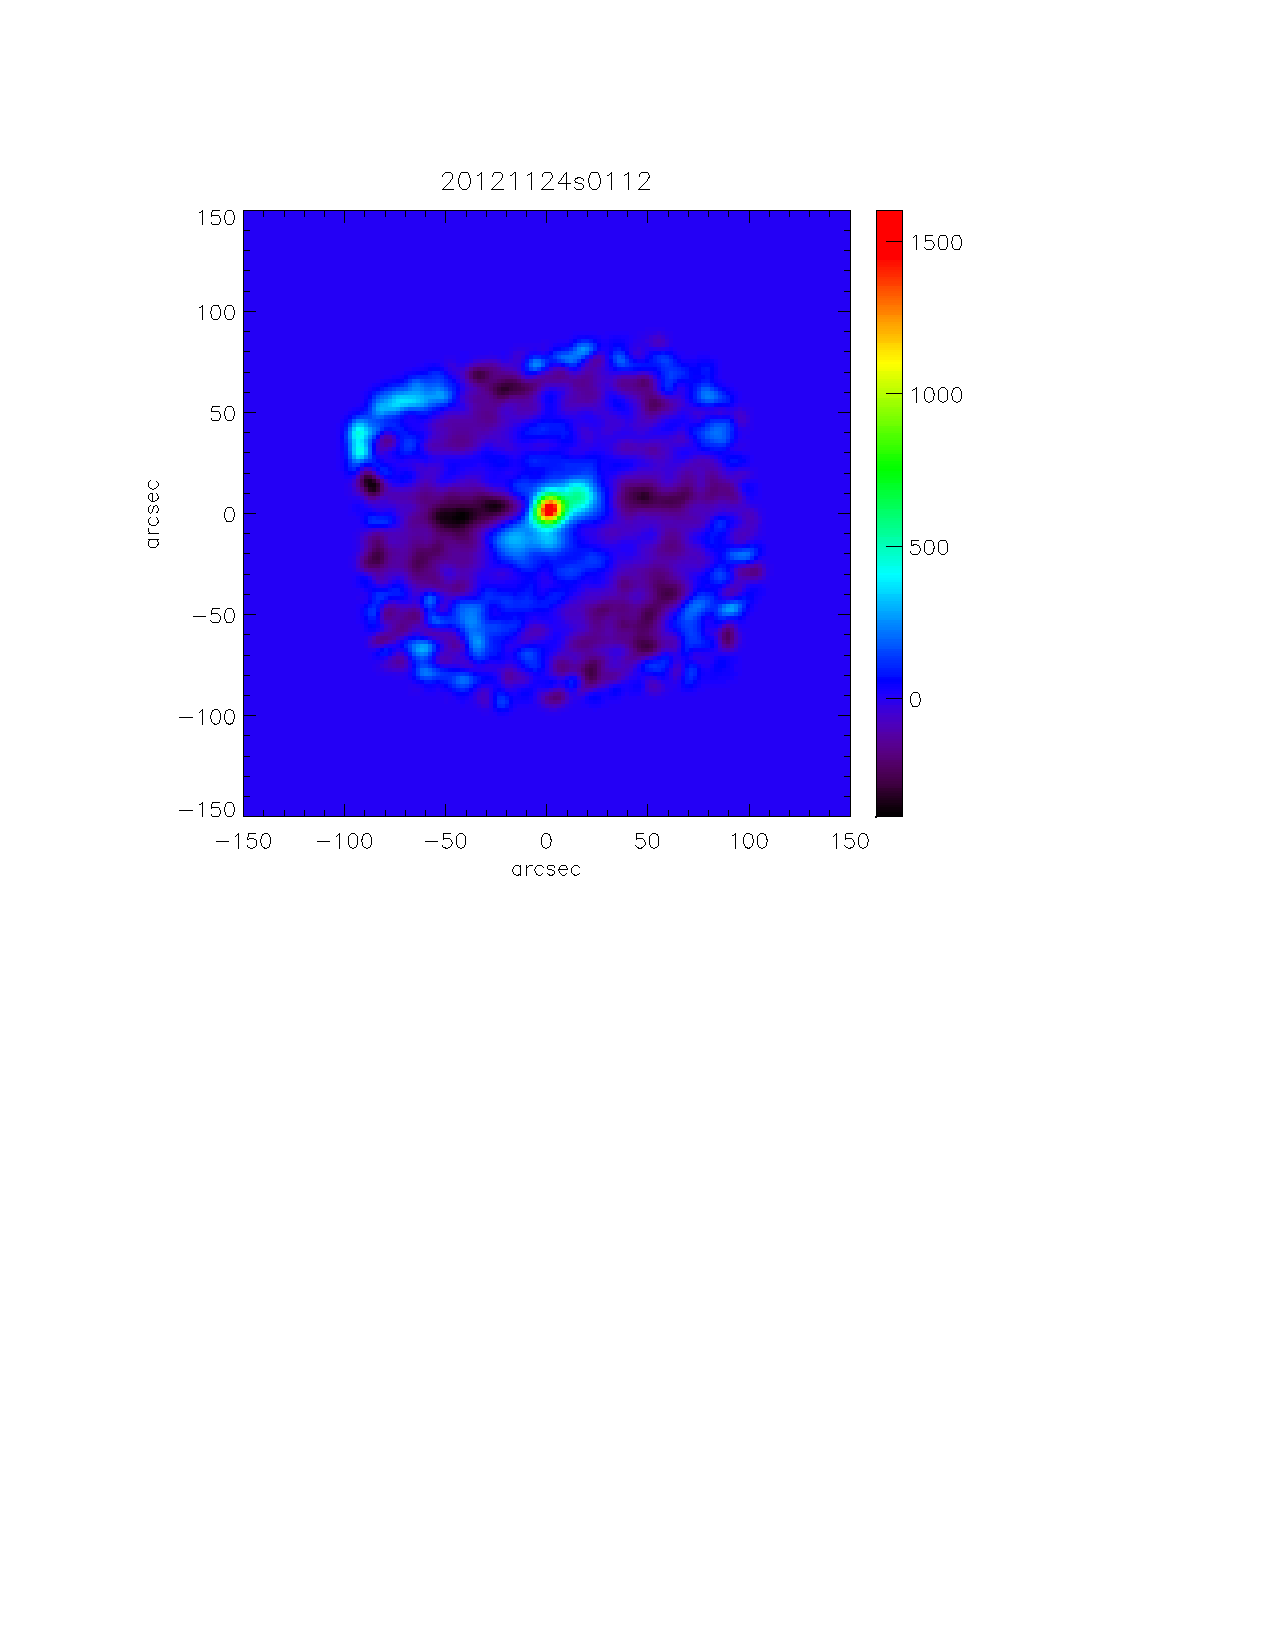
\includegraphics[height=3cm, trim=2cm 13cm 4cm 2cm, clip=true]{Figure/map_1mm_scan20121124s0112}
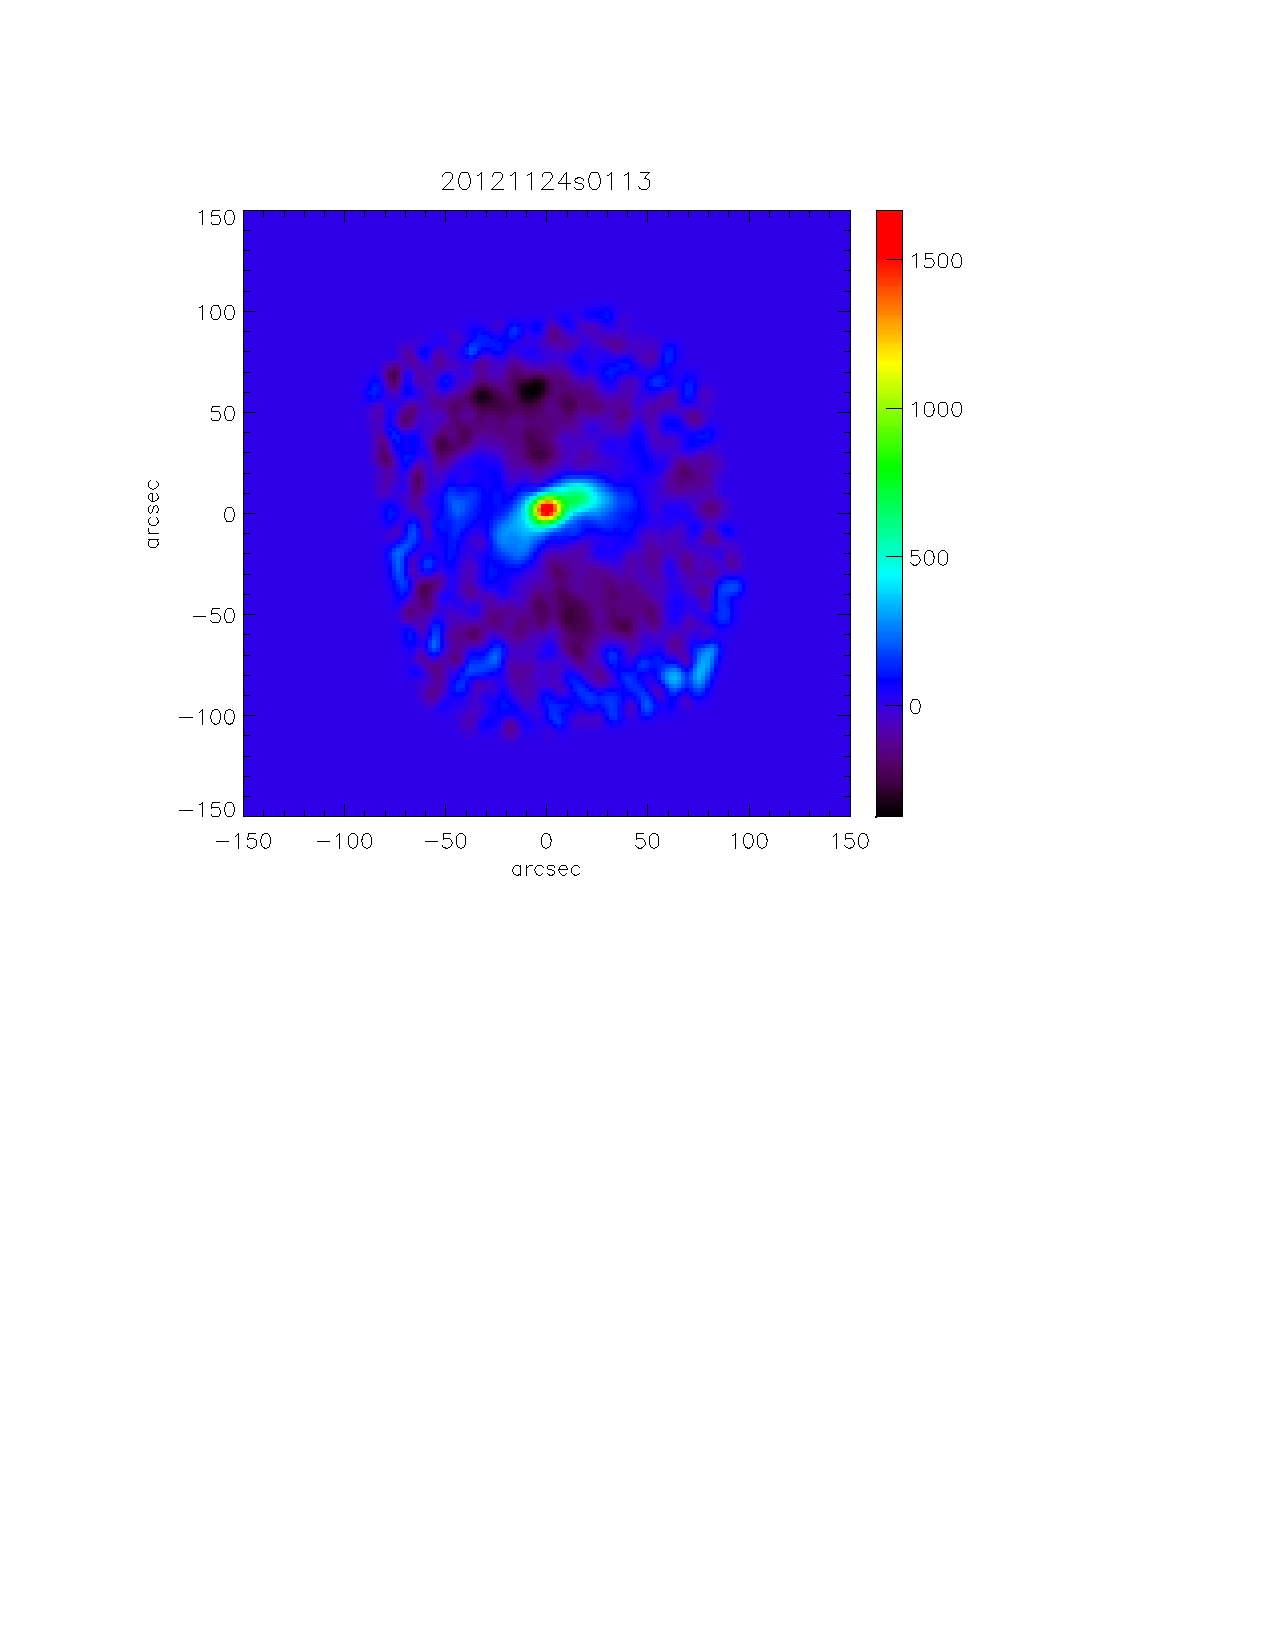
\includegraphics[height=3cm, trim=2cm 13cm 4cm 2cm, clip=true]{Figure/map_1mm_scan20121124s0113}
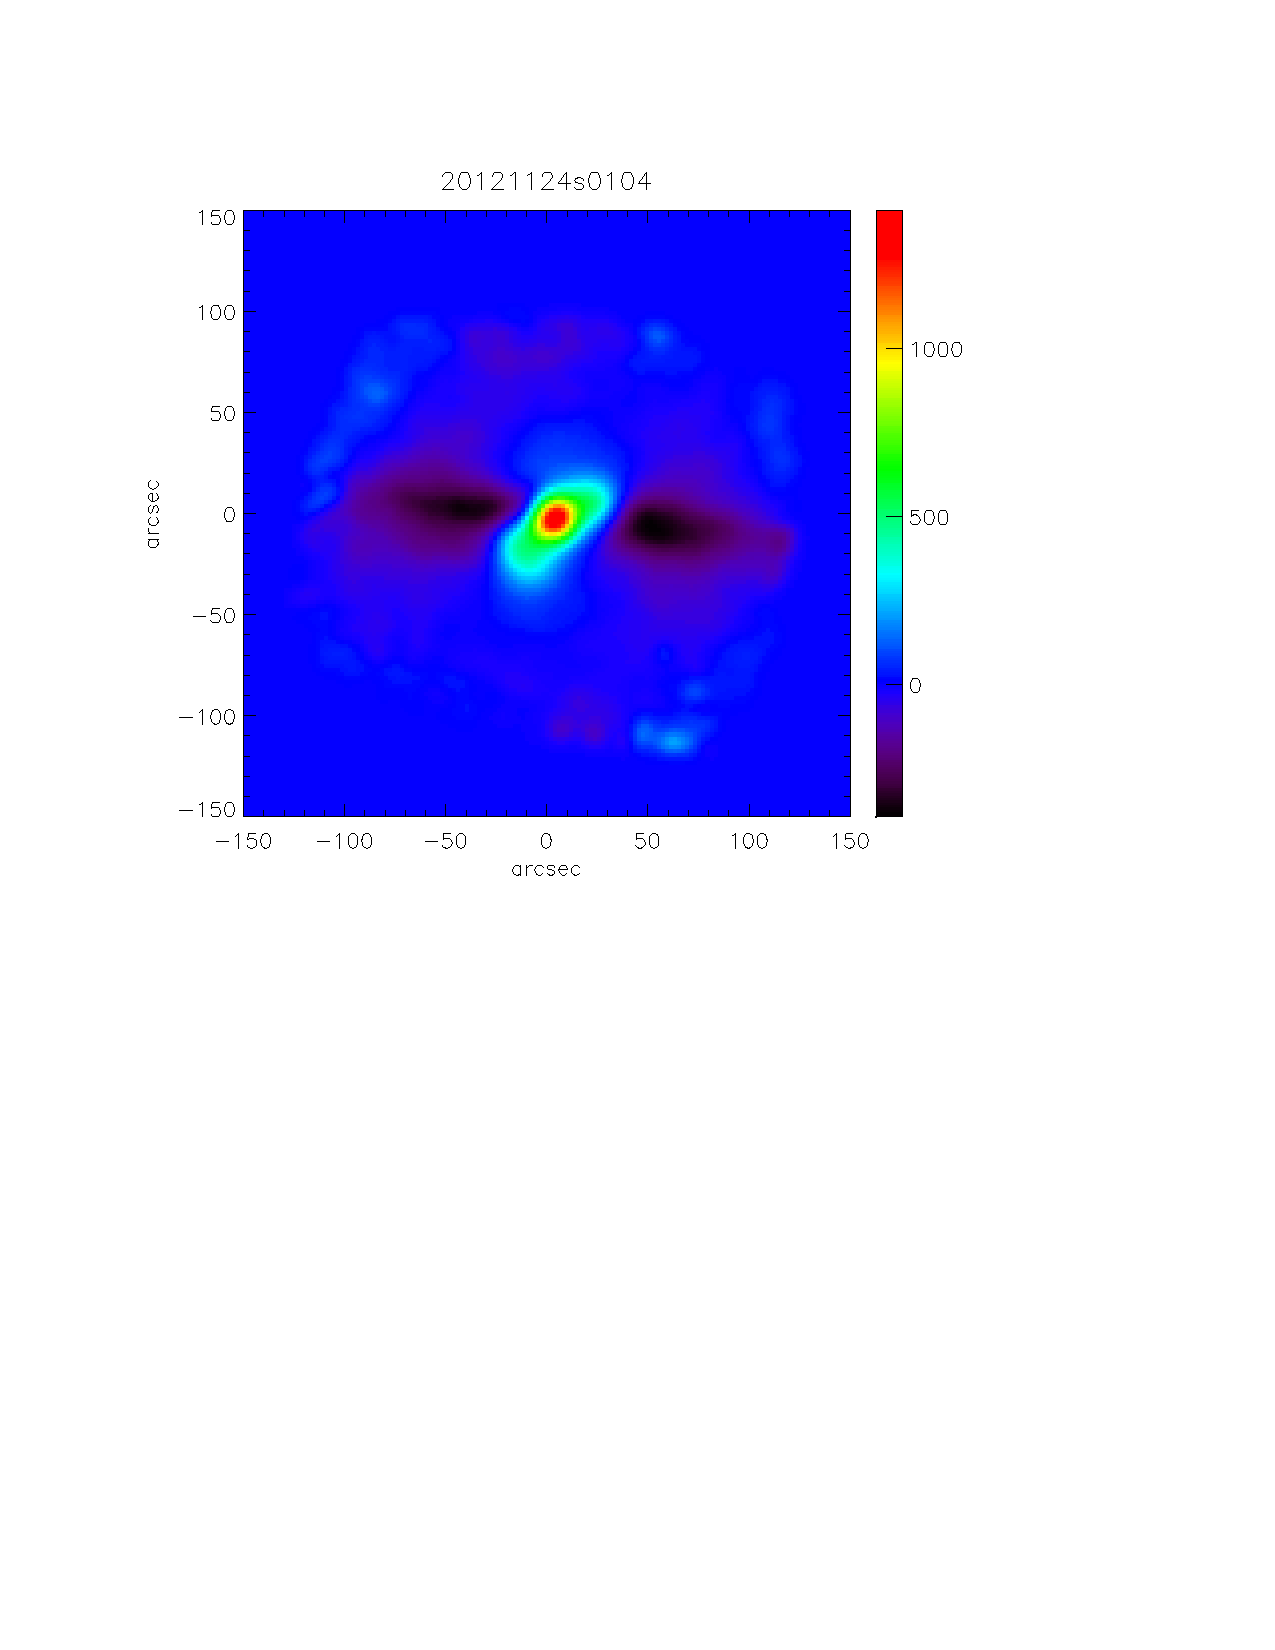
\includegraphics[height=3cm, trim=2cm 13cm 4cm 2cm, clip=true]{Figure/map_2mm_scan20121124s0104}
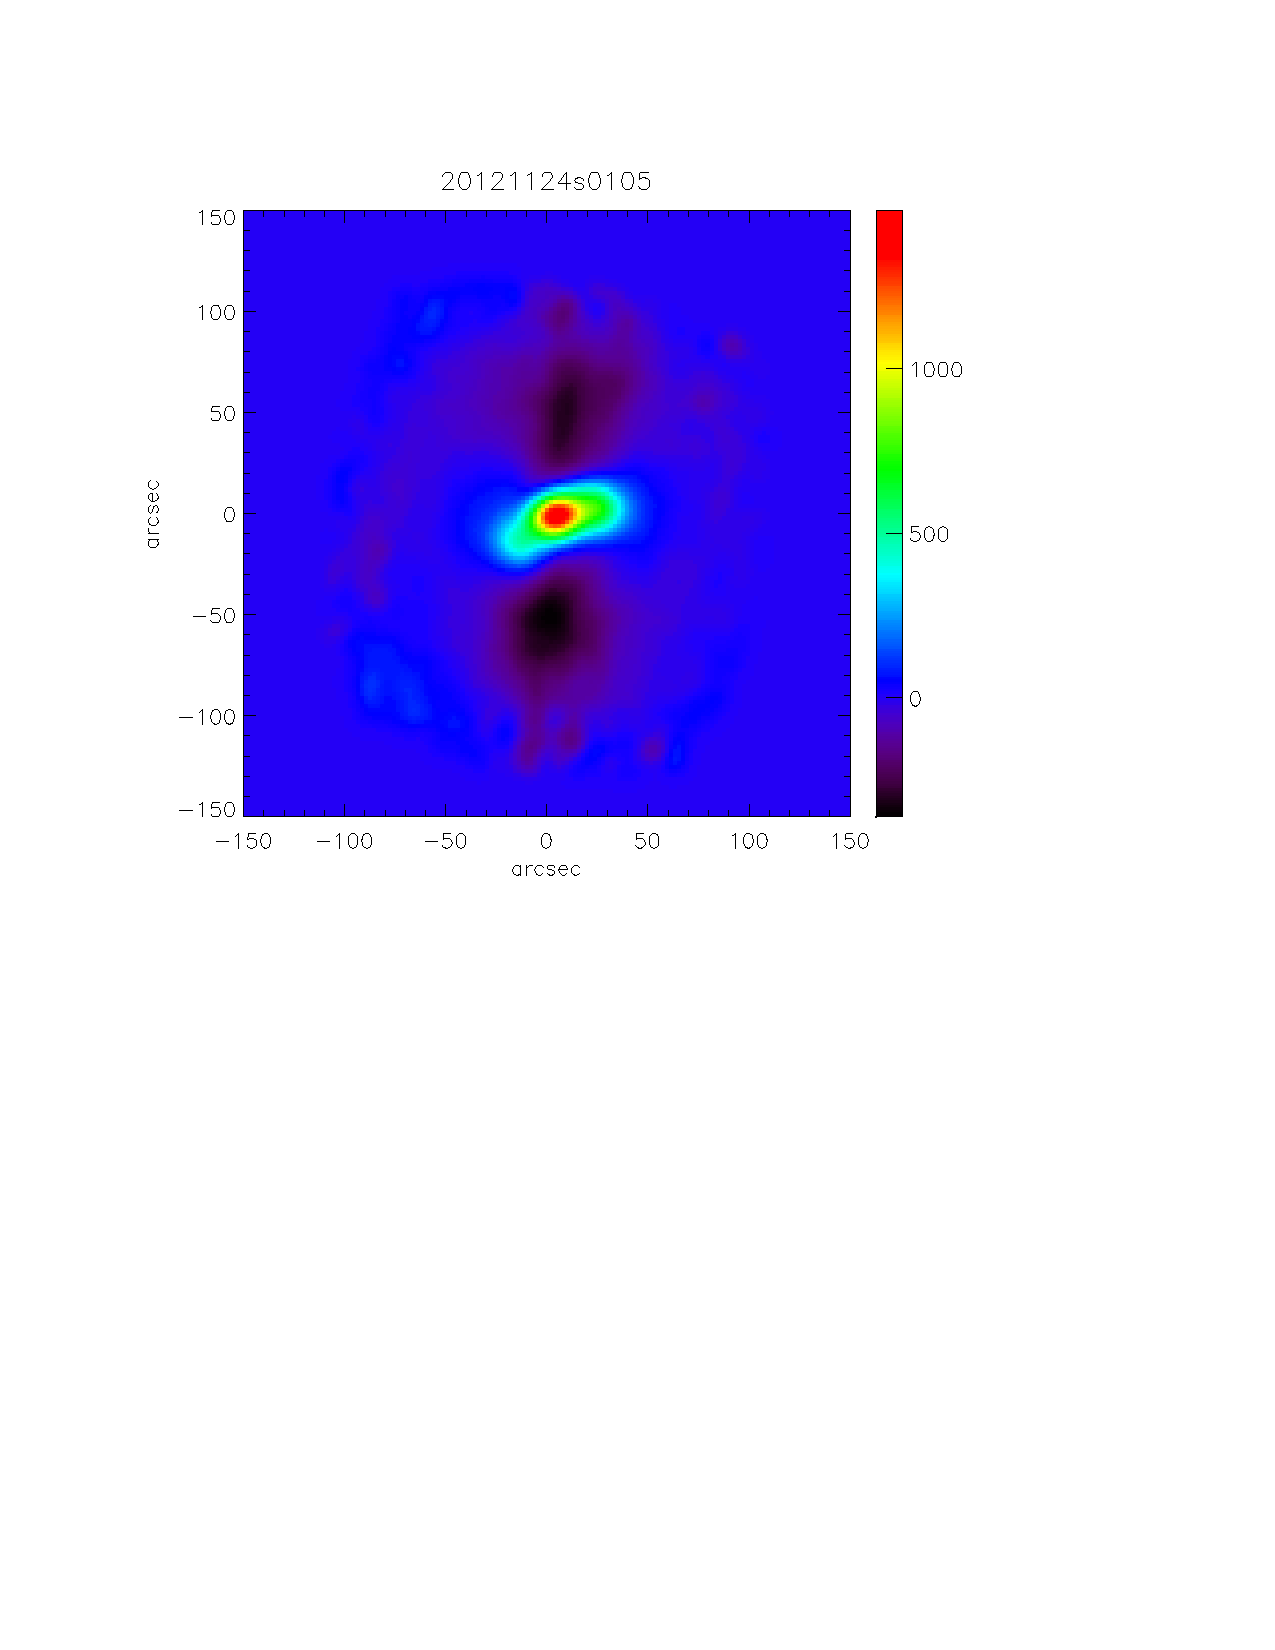
\includegraphics[height=3cm, trim=2cm 13cm 4cm 2cm, clip=true]{Figure/map_2mm_scan20121124s0105}
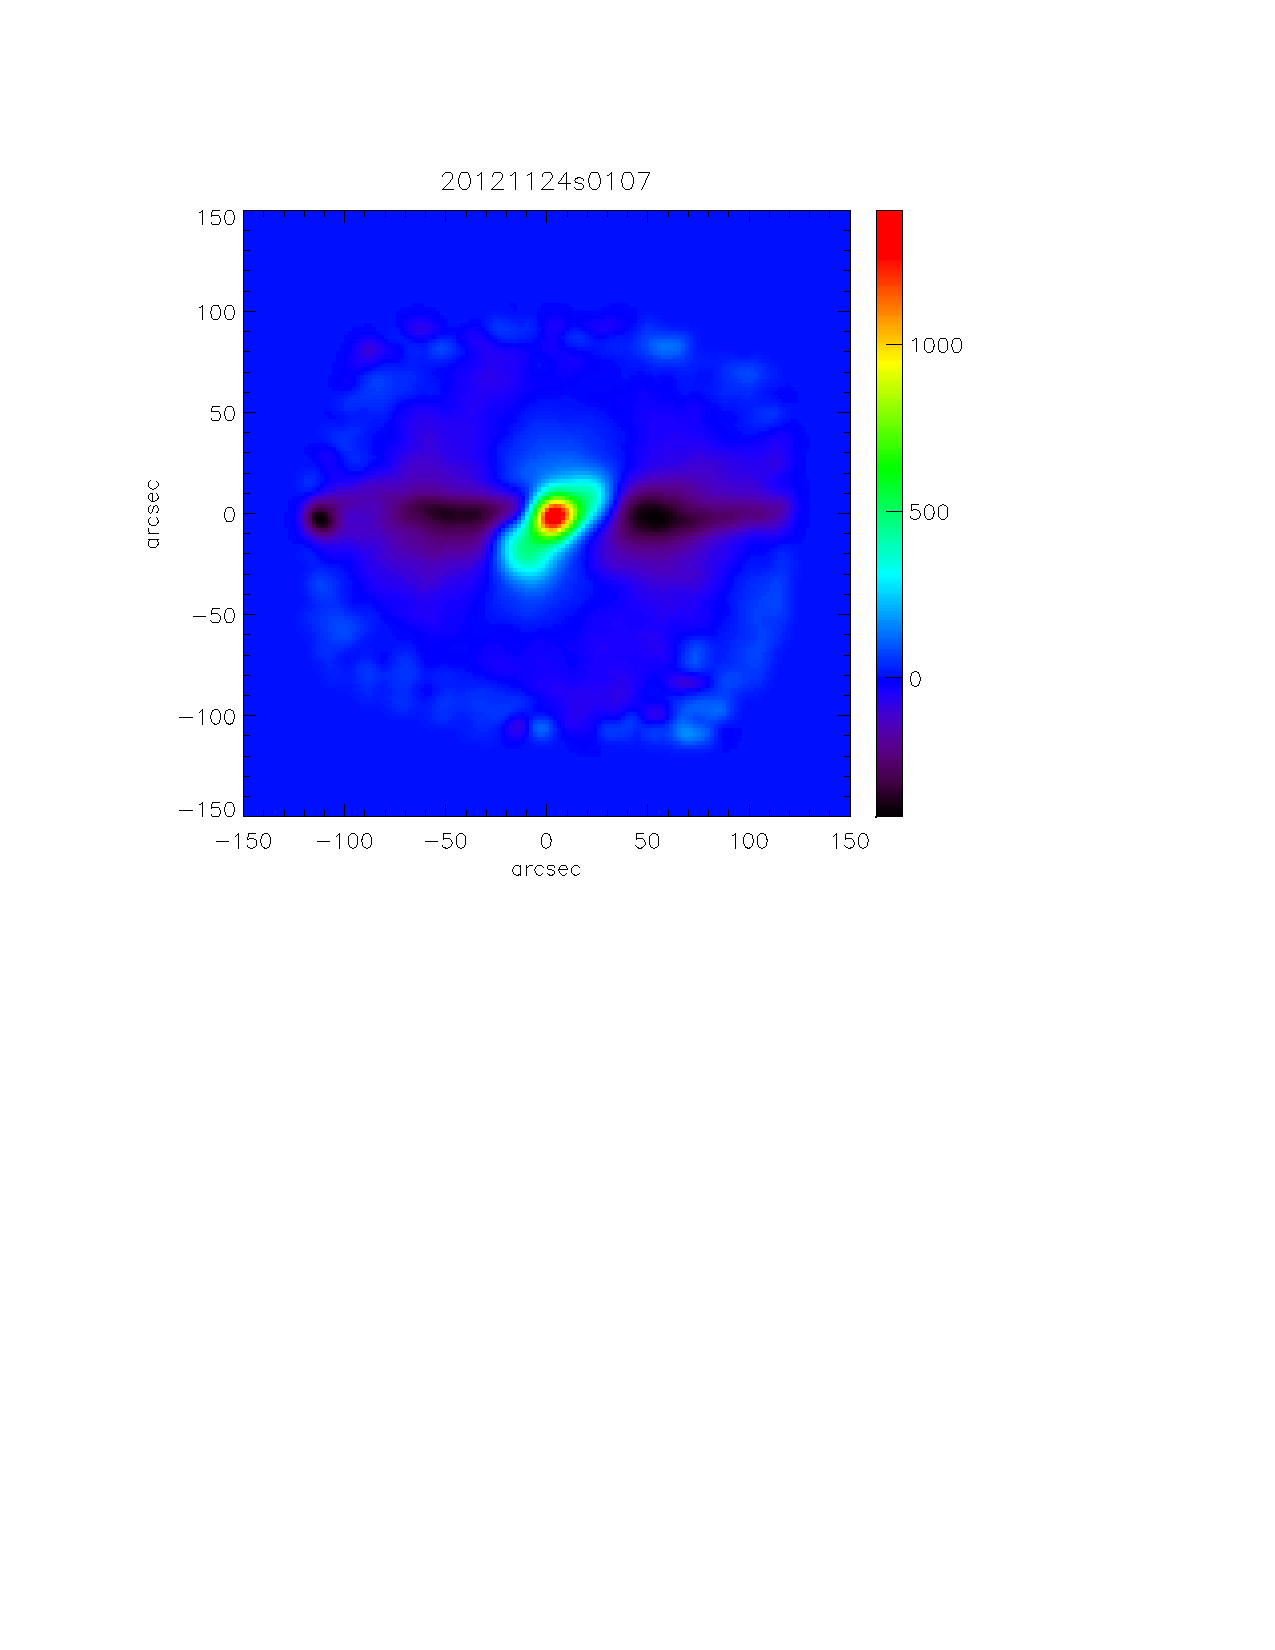
\includegraphics[height=3cm, trim=2cm 13cm 4cm 2cm, clip=true]{Figure/map_2mm_scan20121124s0107}
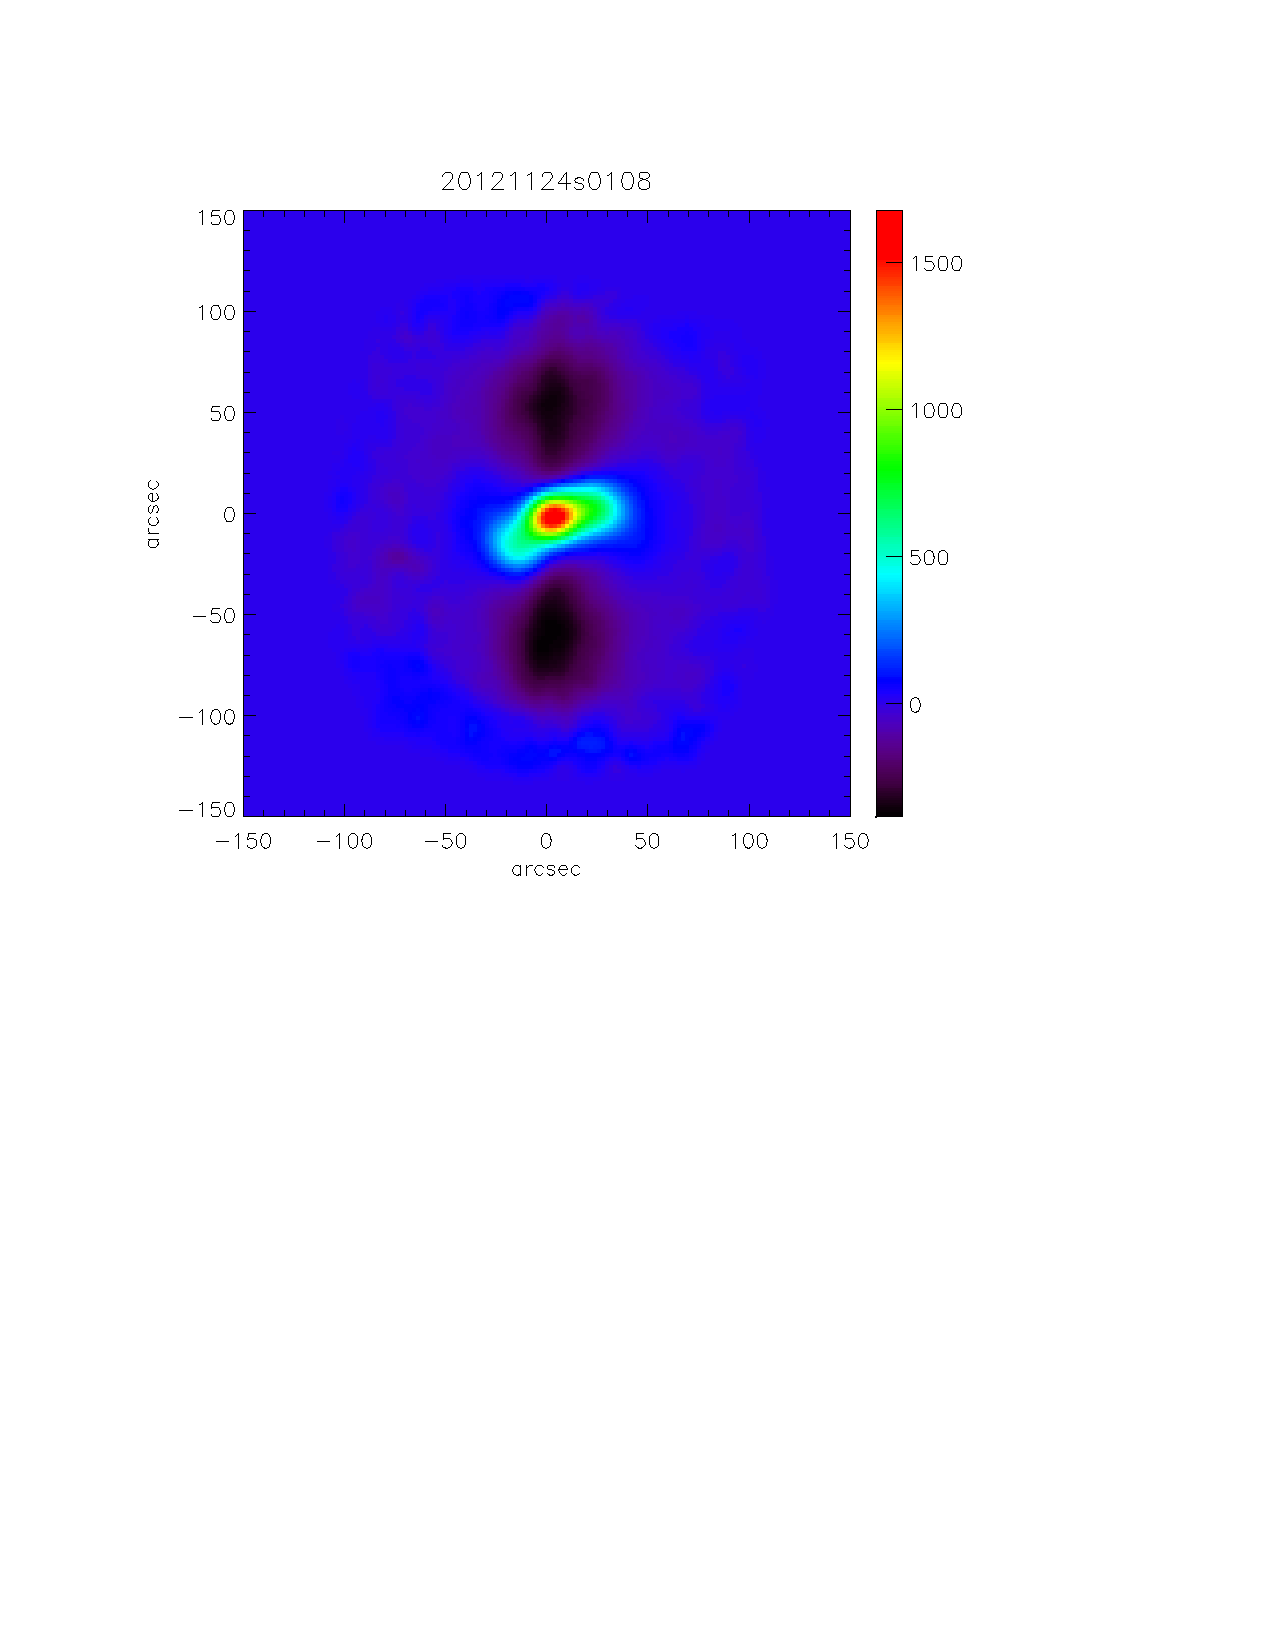
\includegraphics[height=3cm, trim=2cm 13cm 4cm 2cm, clip=true]{Figure/map_2mm_scan20121124s0108}
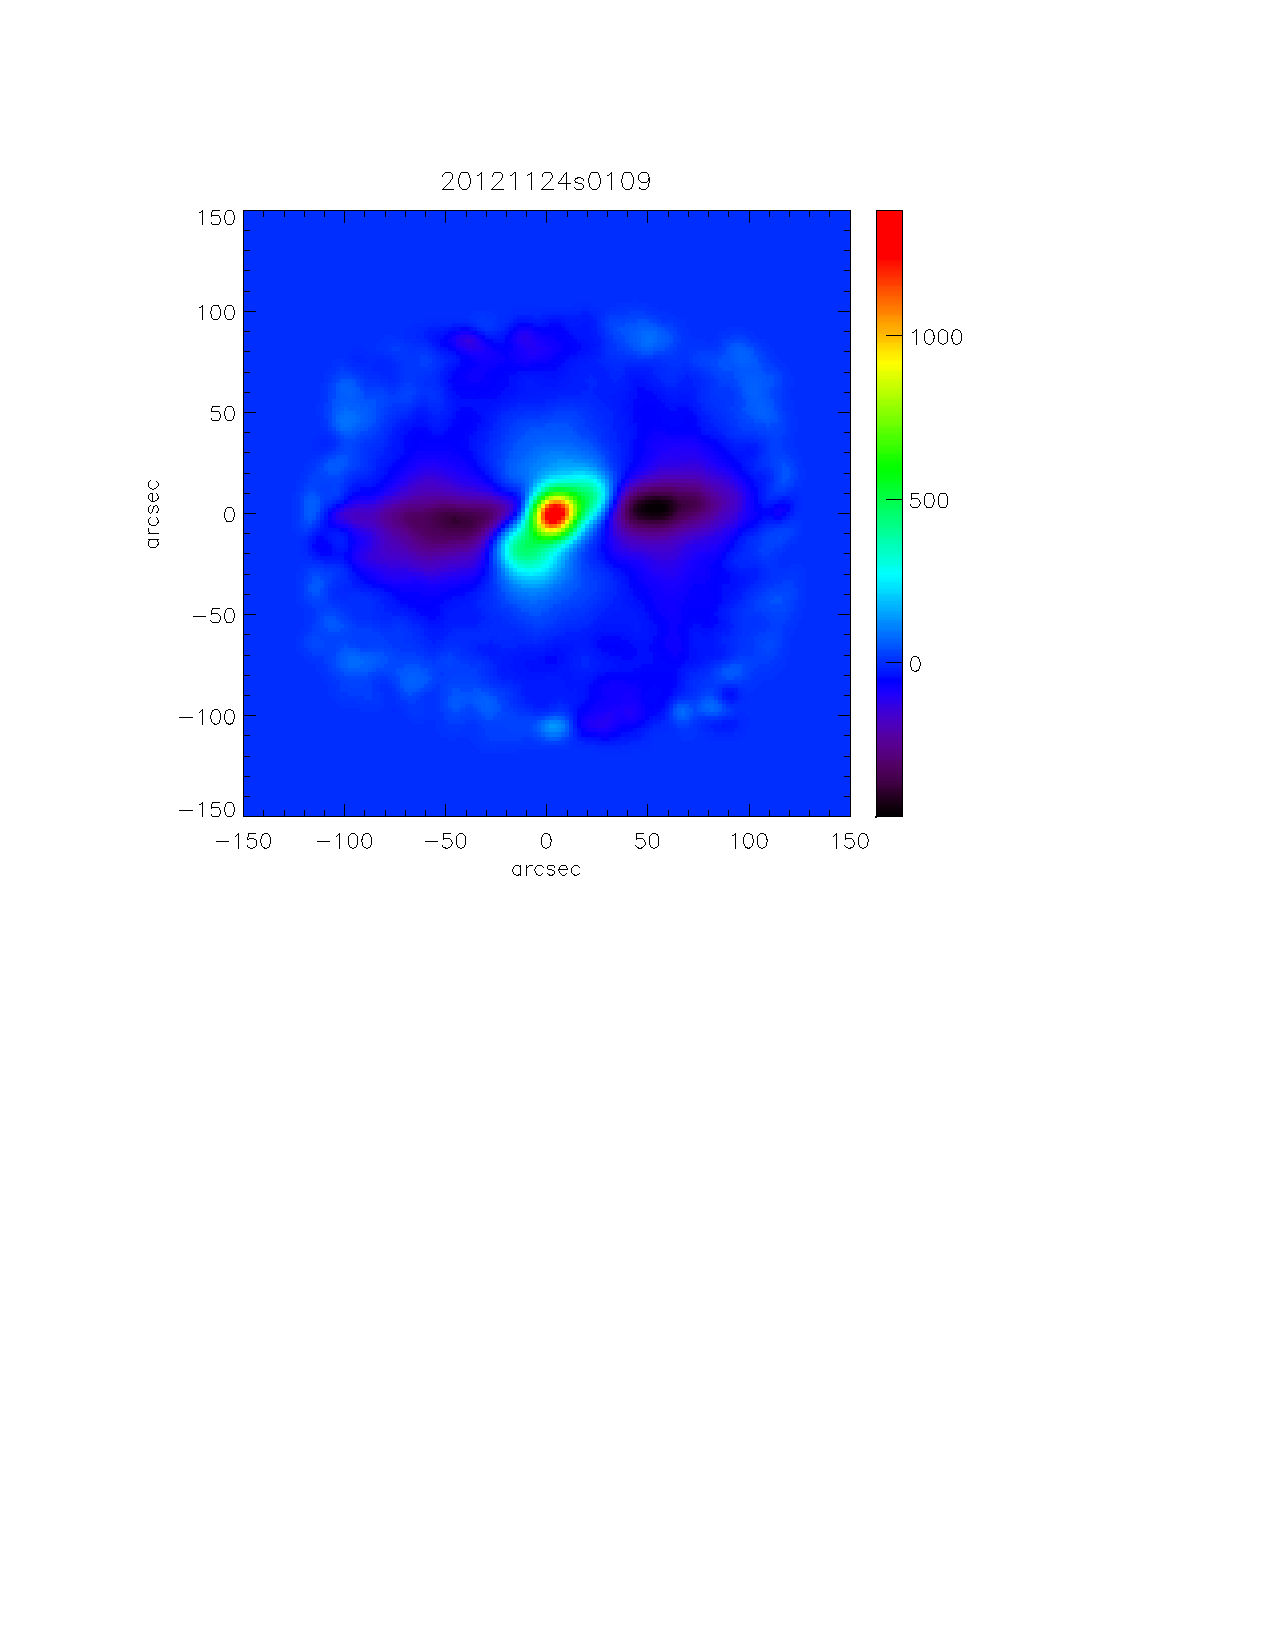
\includegraphics[height=3cm, trim=2cm 13cm 4cm 2cm, clip=true]{Figure/map_2mm_scan20121124s0109}
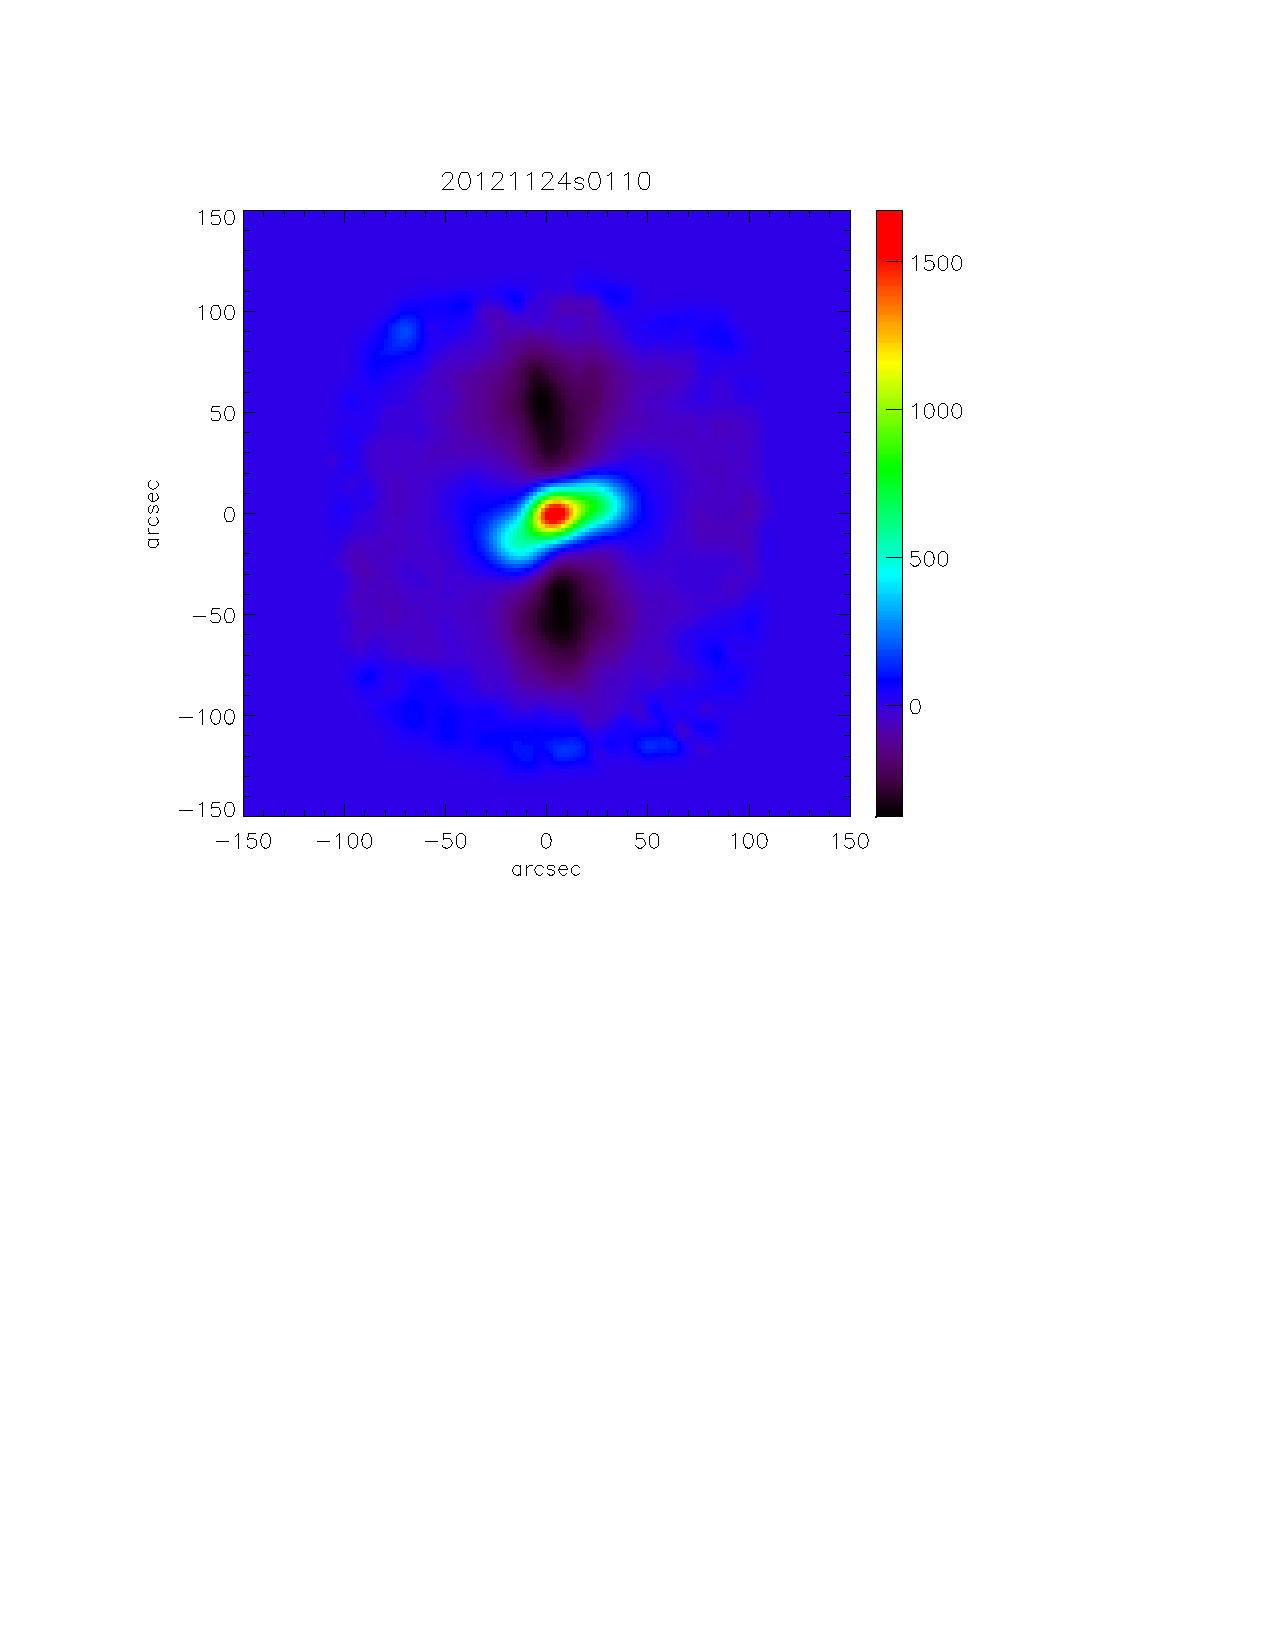
\includegraphics[height=3cm, trim=2cm 13cm 4cm 2cm, clip=true]{Figure/map_2mm_scan20121124s0110}
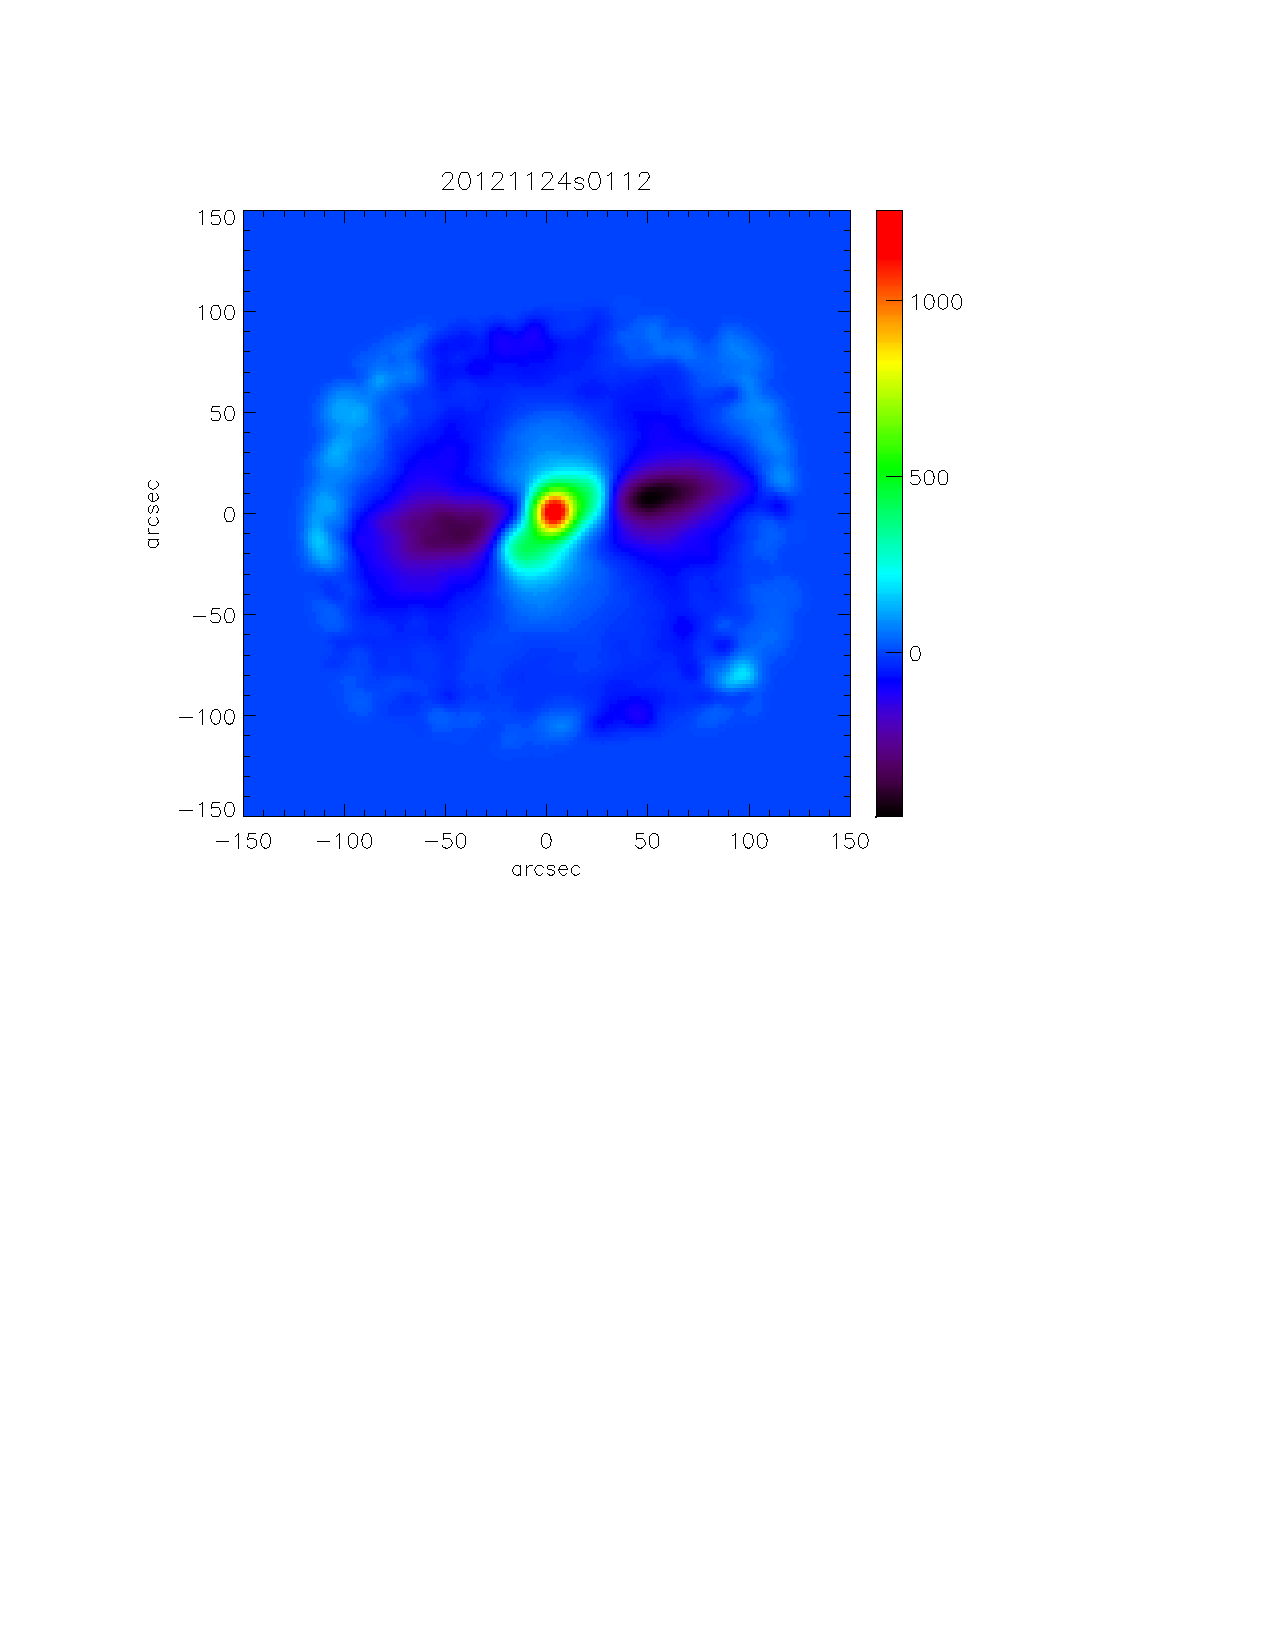
\includegraphics[height=3cm, trim=2cm 13cm 4cm 2cm, clip=true]{Figure/map_2mm_scan20121124s0112}
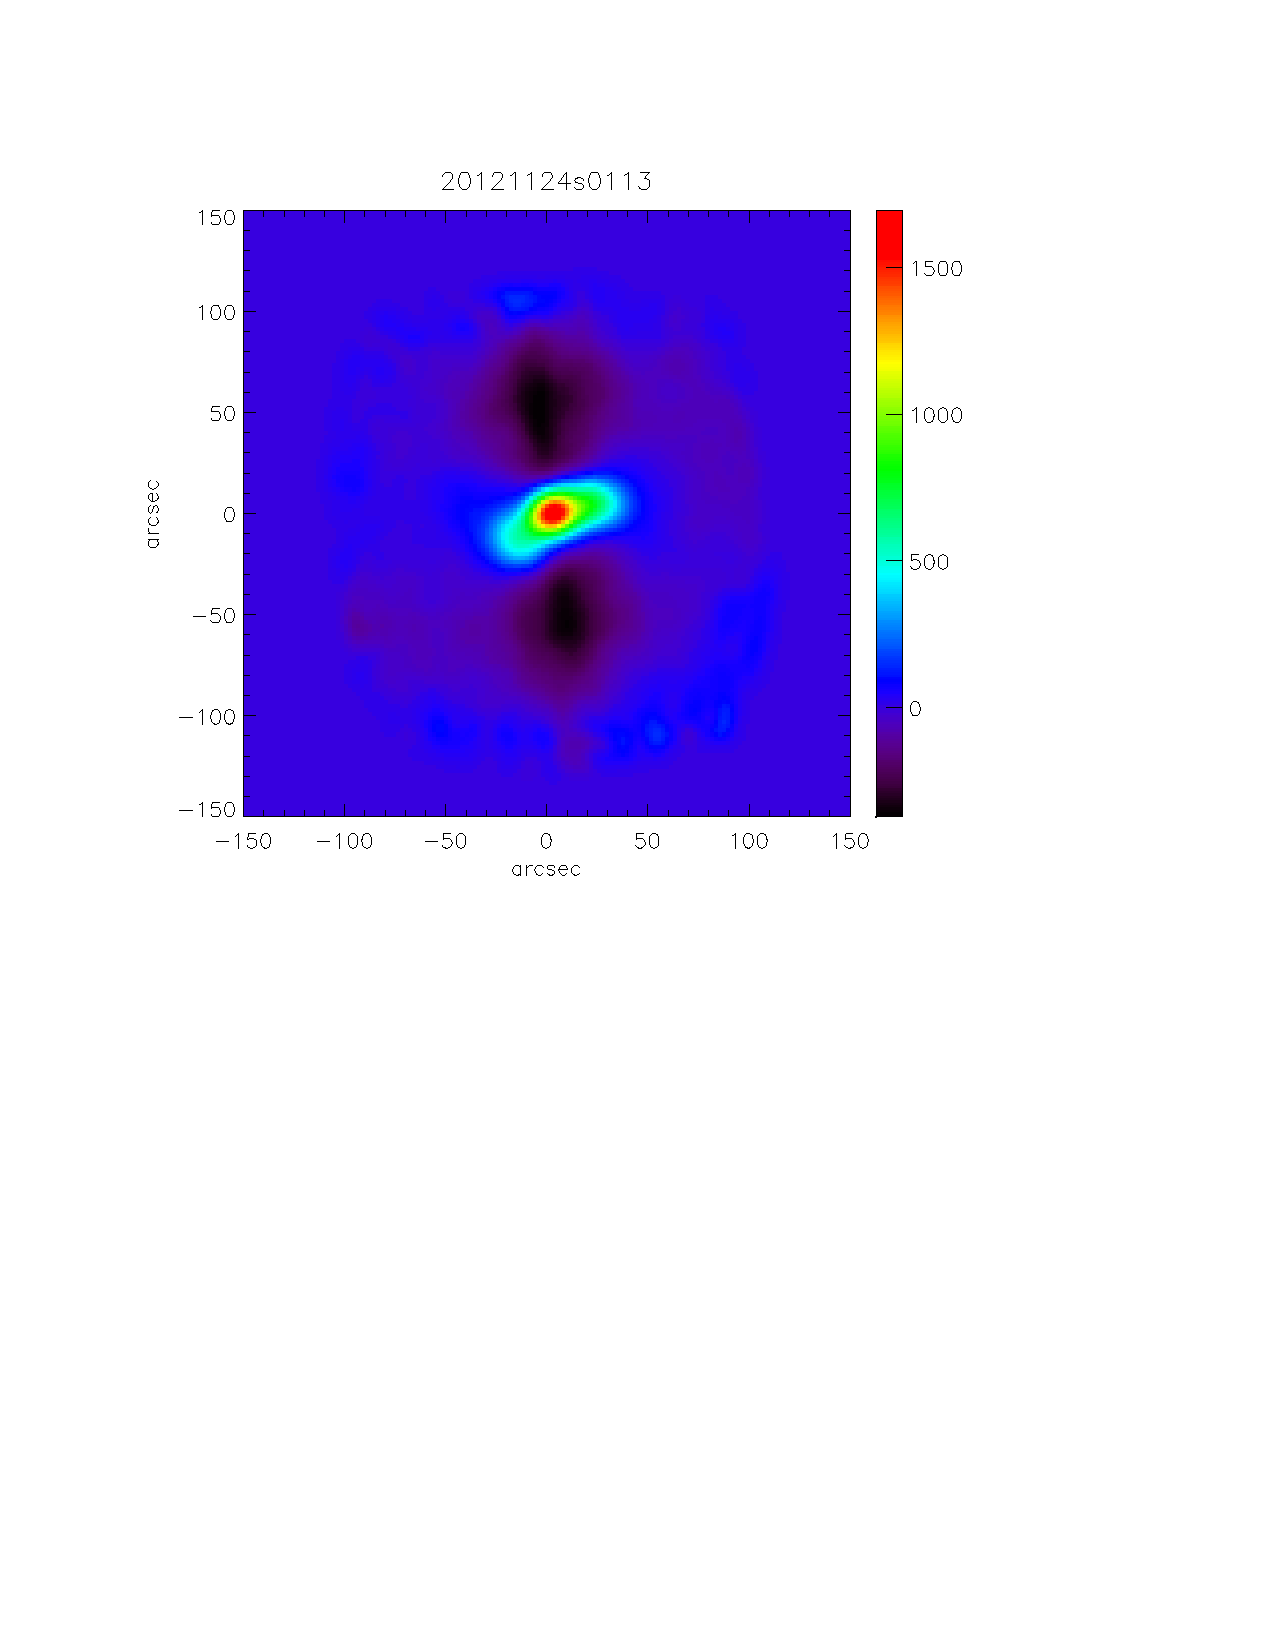
\includegraphics[height=3cm, trim=2cm 13cm 4cm 2cm, clip=true]{Figure/map_2mm_scan20121124s0113}
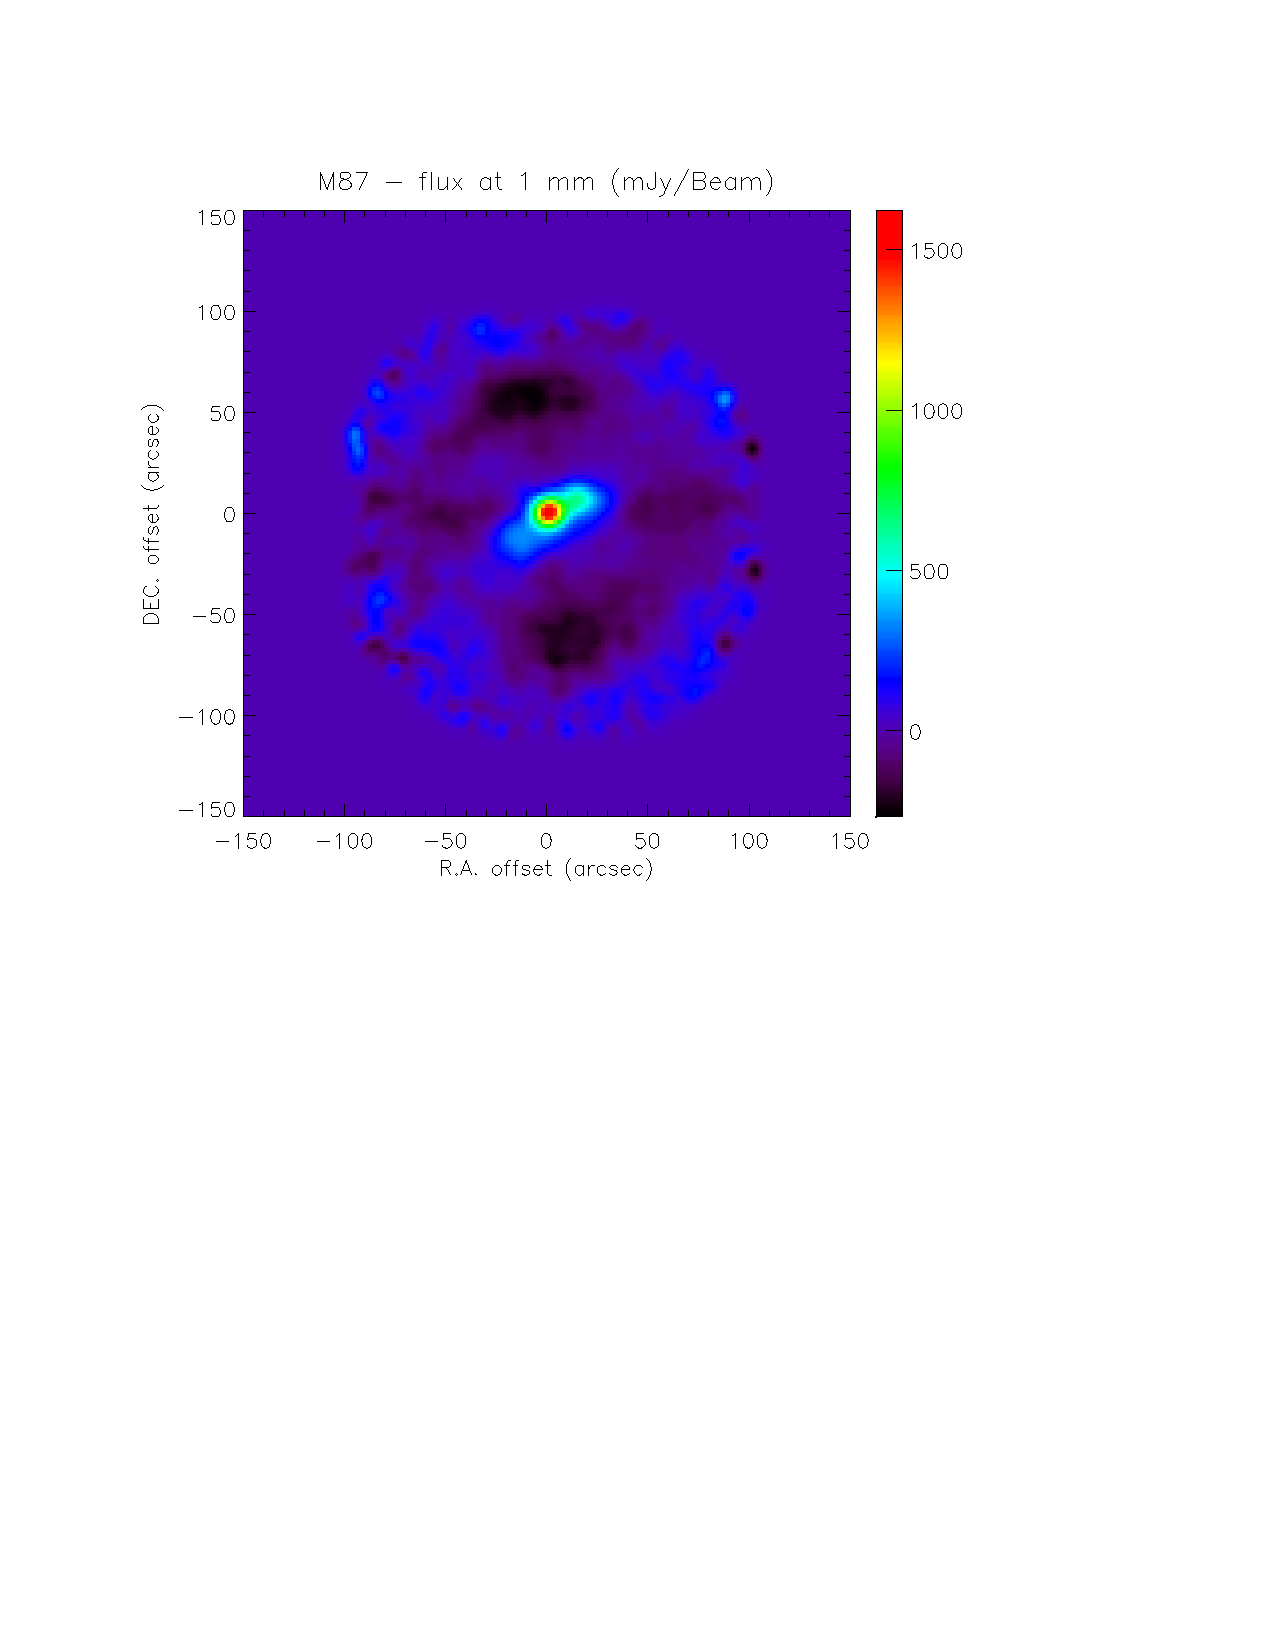
\includegraphics[height=6cm, trim=2cm 13cm 4cm 2cm, clip=true]{Figure/M87_flux_map_1mm}
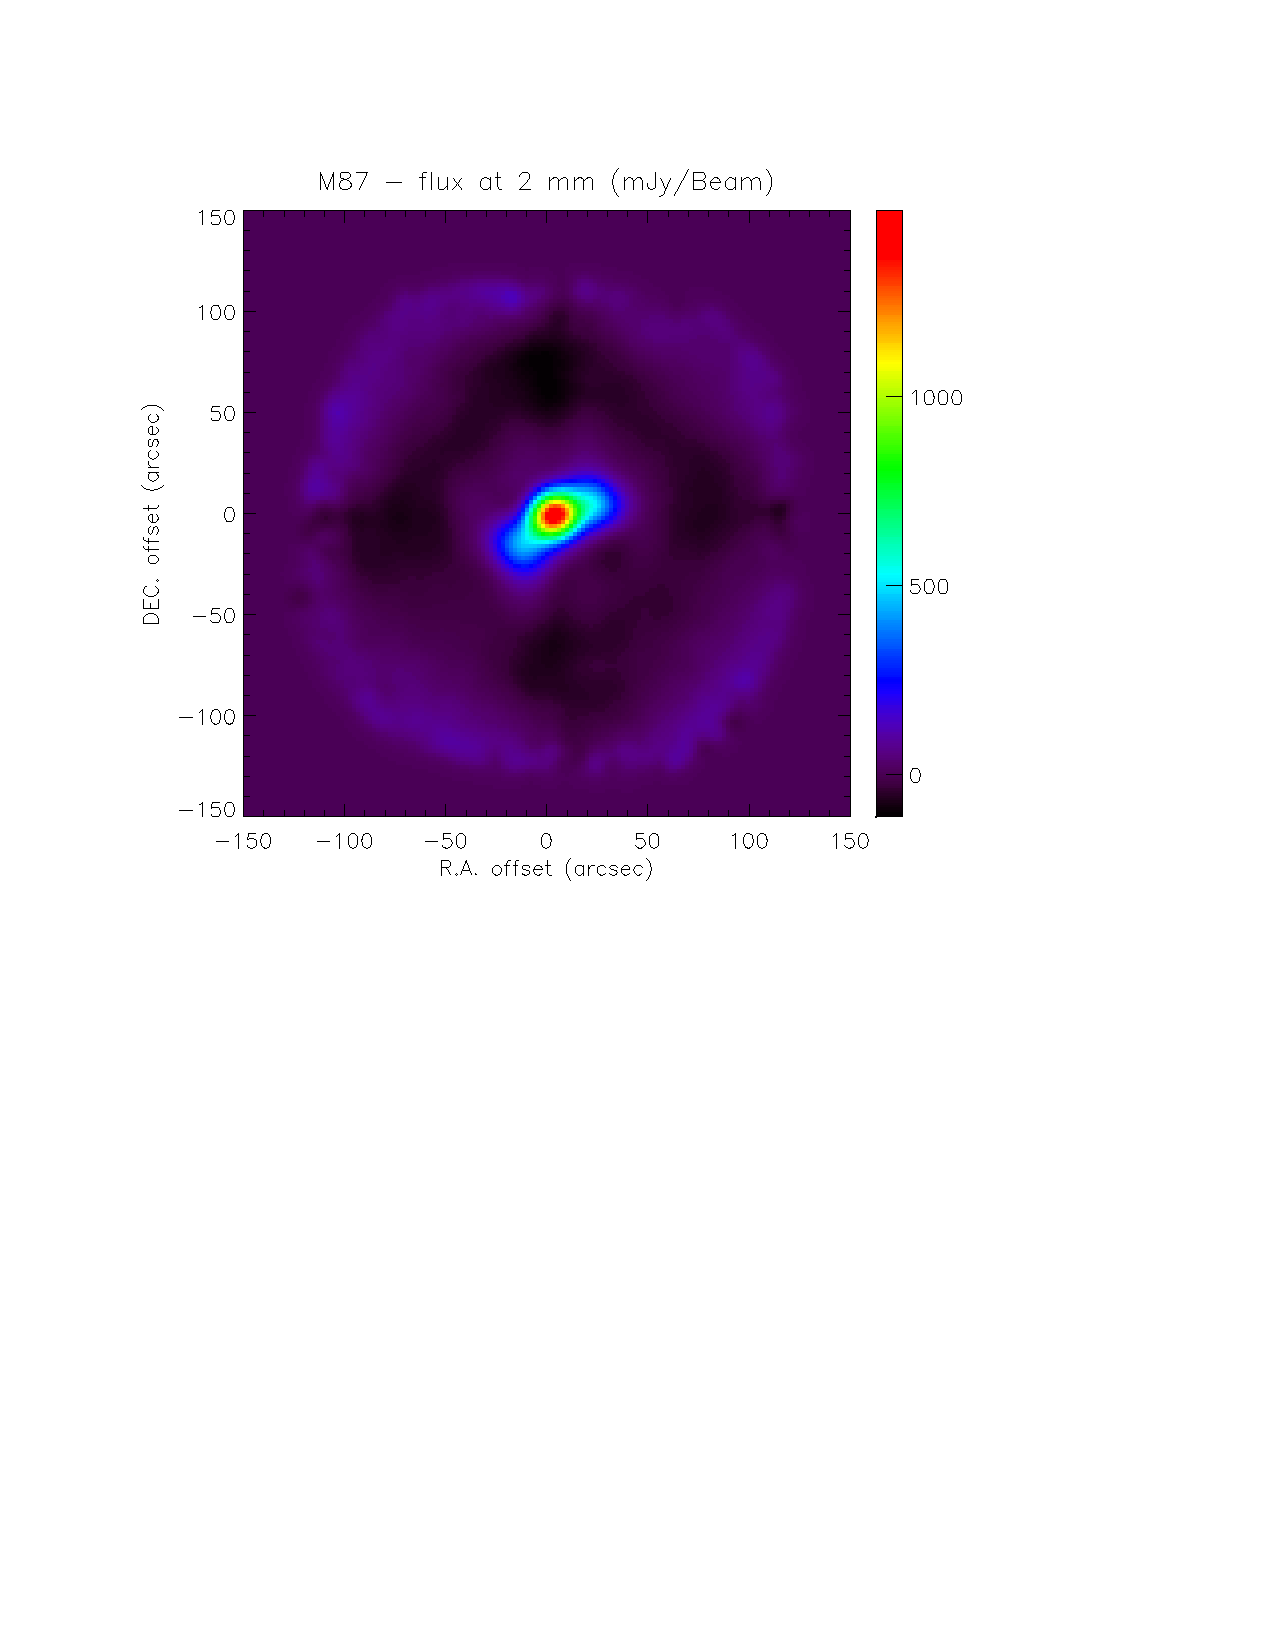
\includegraphics[height=6cm, trim=2cm 13cm 4cm 2cm, clip=true]{Figure/M87_flux_map_2mm}
\caption{Individual scan maps for both wavelength in the case of M87. The two first row are at at 1mm and the row 3 and 4 at 2mm. The odd scans are along the azimuth and the even scans along the elevation. The negative lobes are due to the decorrelation and are oriented along the scan direction. The maps are in mJy/Beam. The associated combined maps are shown at the bottom.}
\label{fig:M87_map_per_scan}
\end{figure}

%Time per pixel
In addition to the flux maps, one of the direct output of the pipeline is the time spent per pixel (both in the combined and individual map per scan structures). It is given in the case of this example in Fig.~\ref{fig:M87_time}.
\begin{figure}
\centering
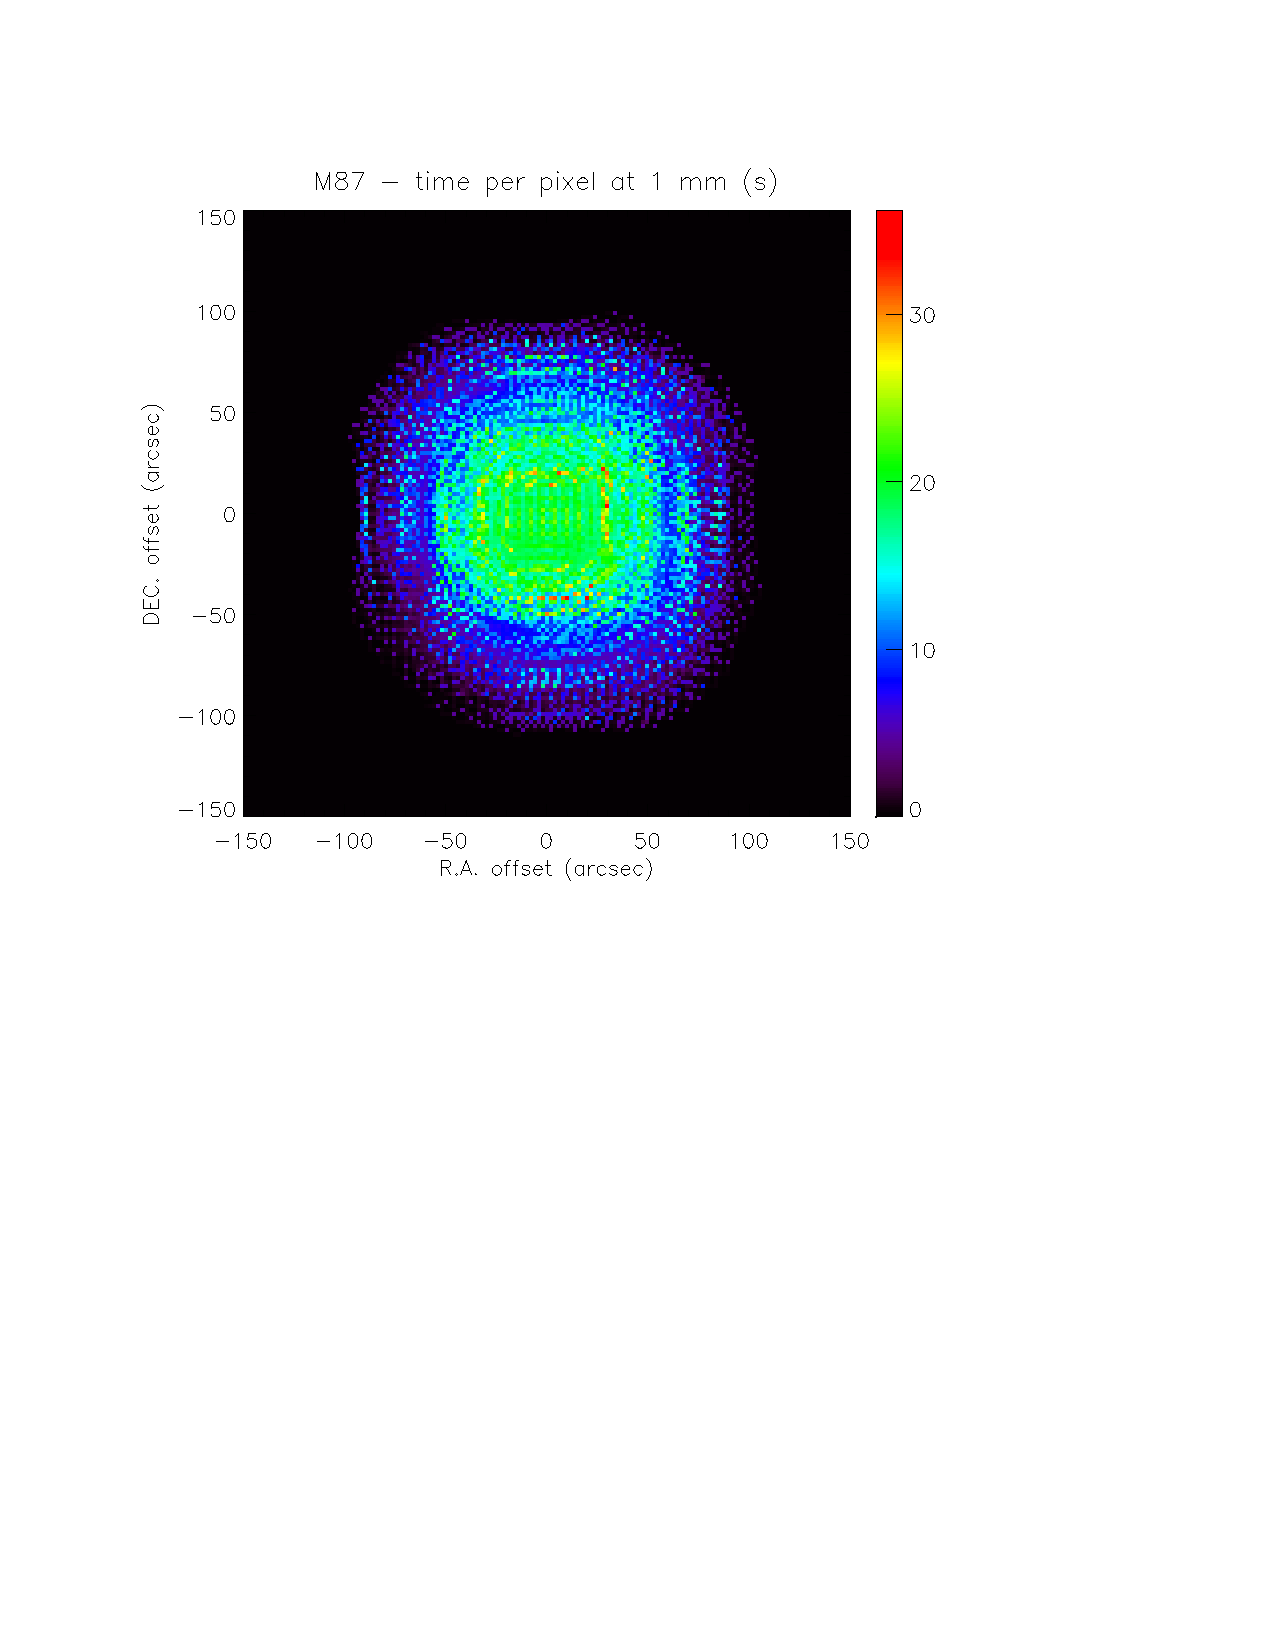
\includegraphics[height=6cm, trim=2cm 13cm 4cm 2cm, clip=true]{Figure/M87_time_map_1mm}
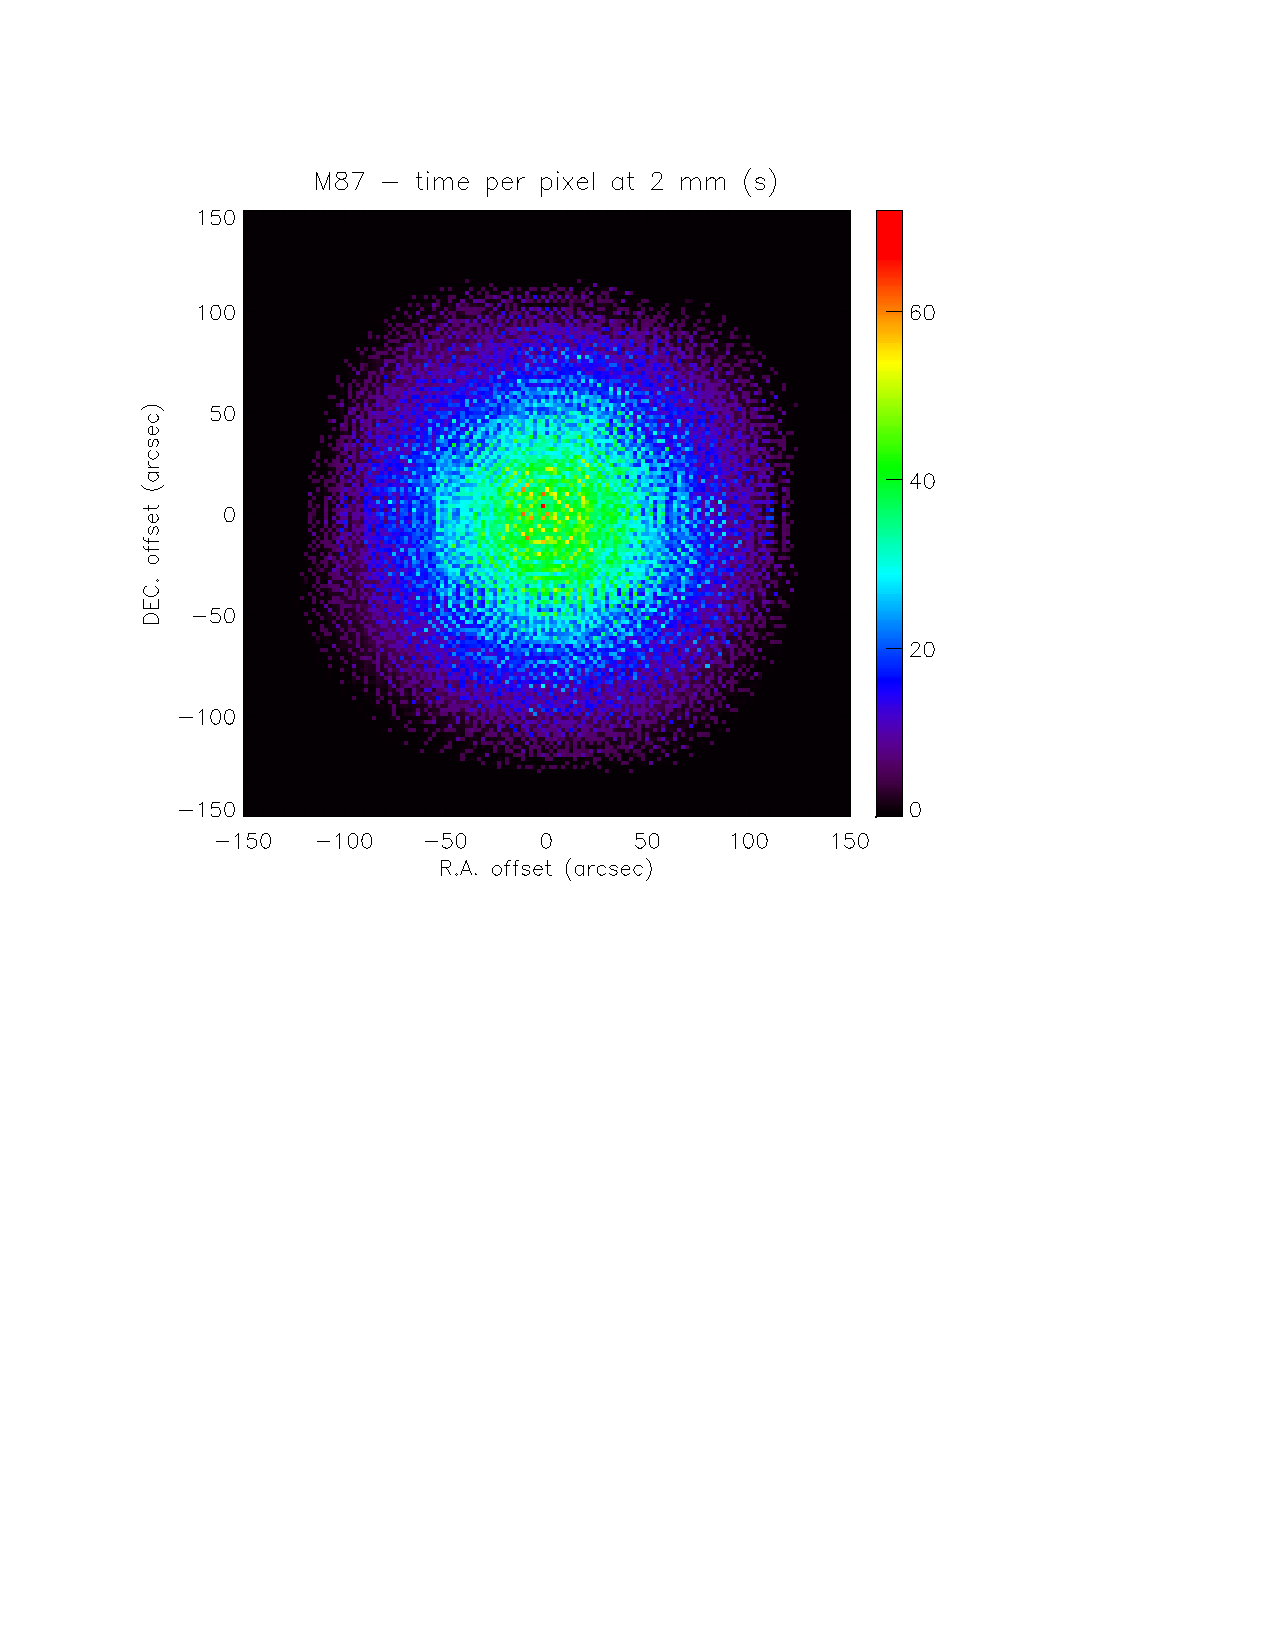
\includegraphics[height=6cm, trim=2cm 13cm 4cm 2cm, clip=true]{Figure/M87_time_map_2mm}
\caption{Time per pixel maps for both arrays.}
\label{fig:M87_time}
\end{figure}

%Jack-knives
Using the individual map per scan, we compute the Jack-Knives by splitting maps set in two equivalent parts. We check that  the residual is much smaller than the signal (see Fig.~\ref{fig:M87_JK}).
\begin{figure}
\centering
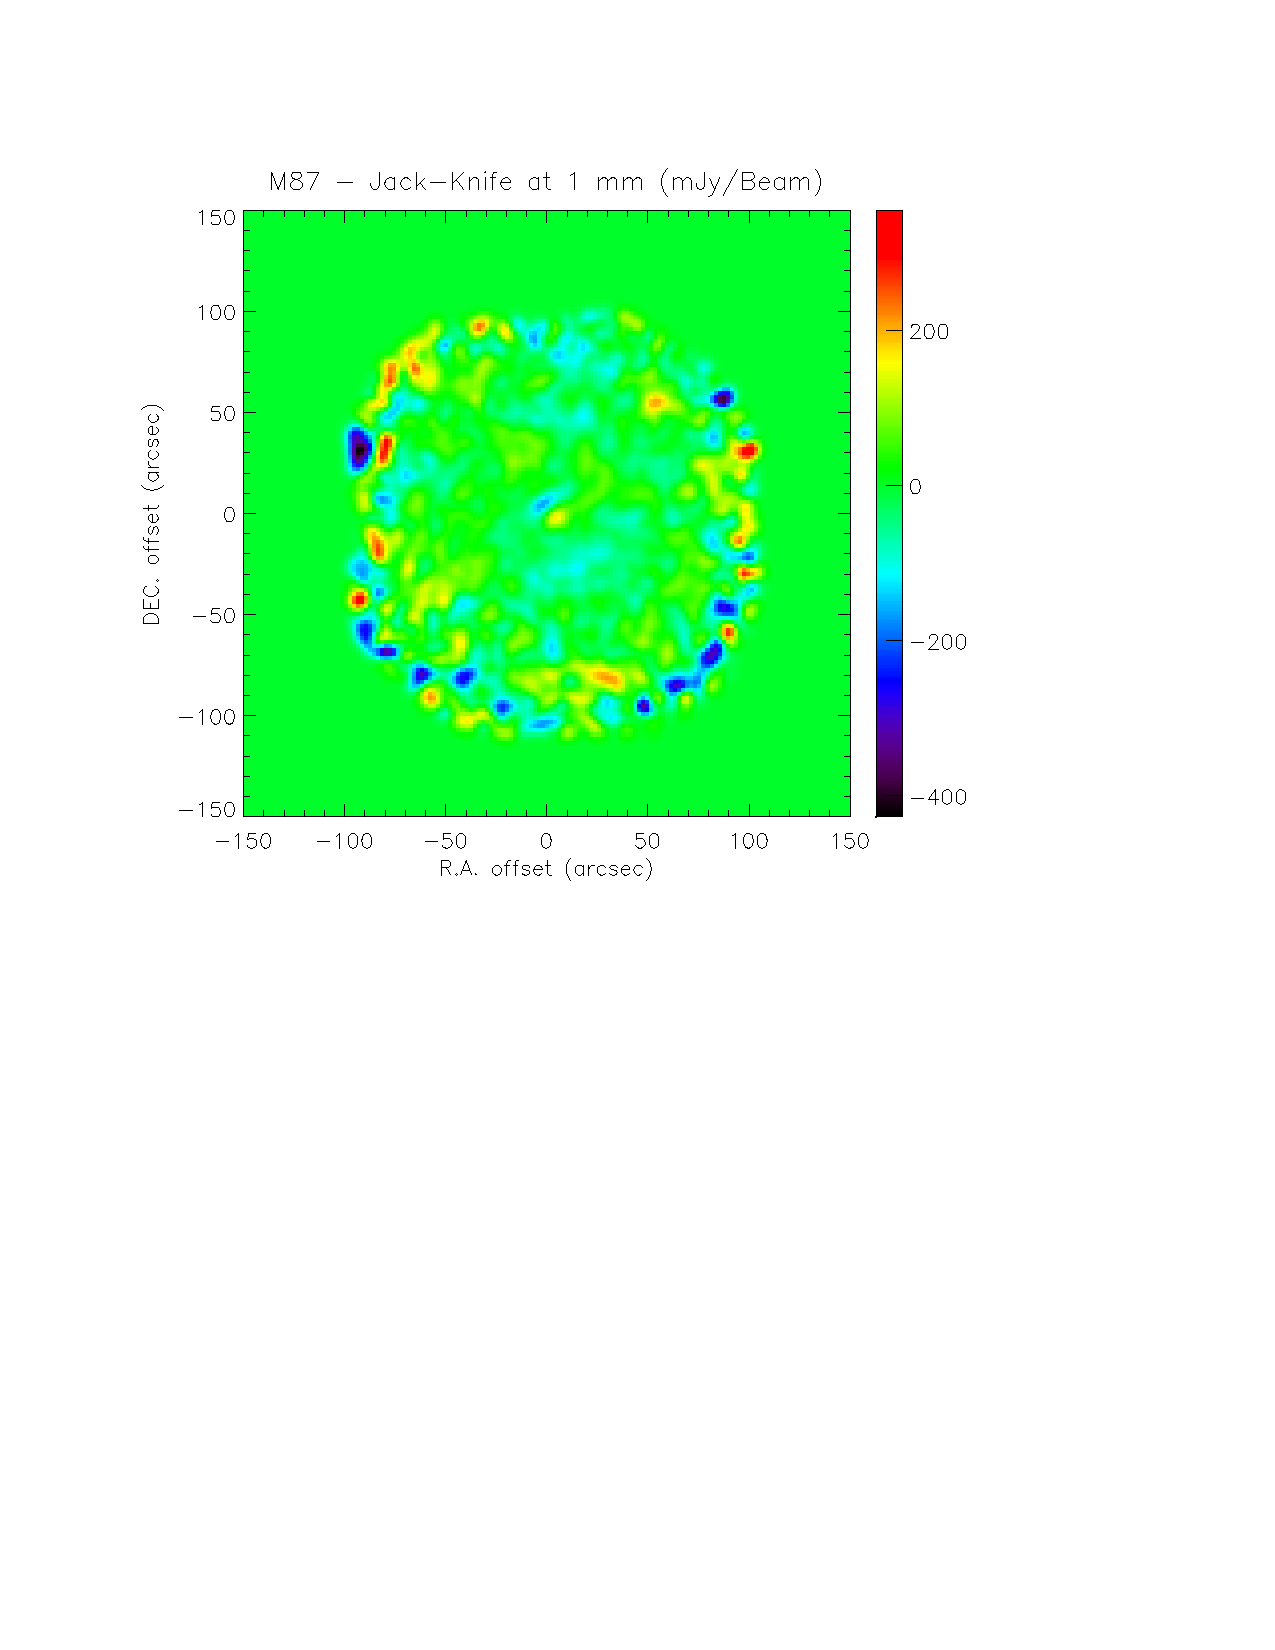
\includegraphics[height=6cm, trim=2cm 13cm 4cm 2cm, clip=true]{Figure/M87_jack-knife_1mm}
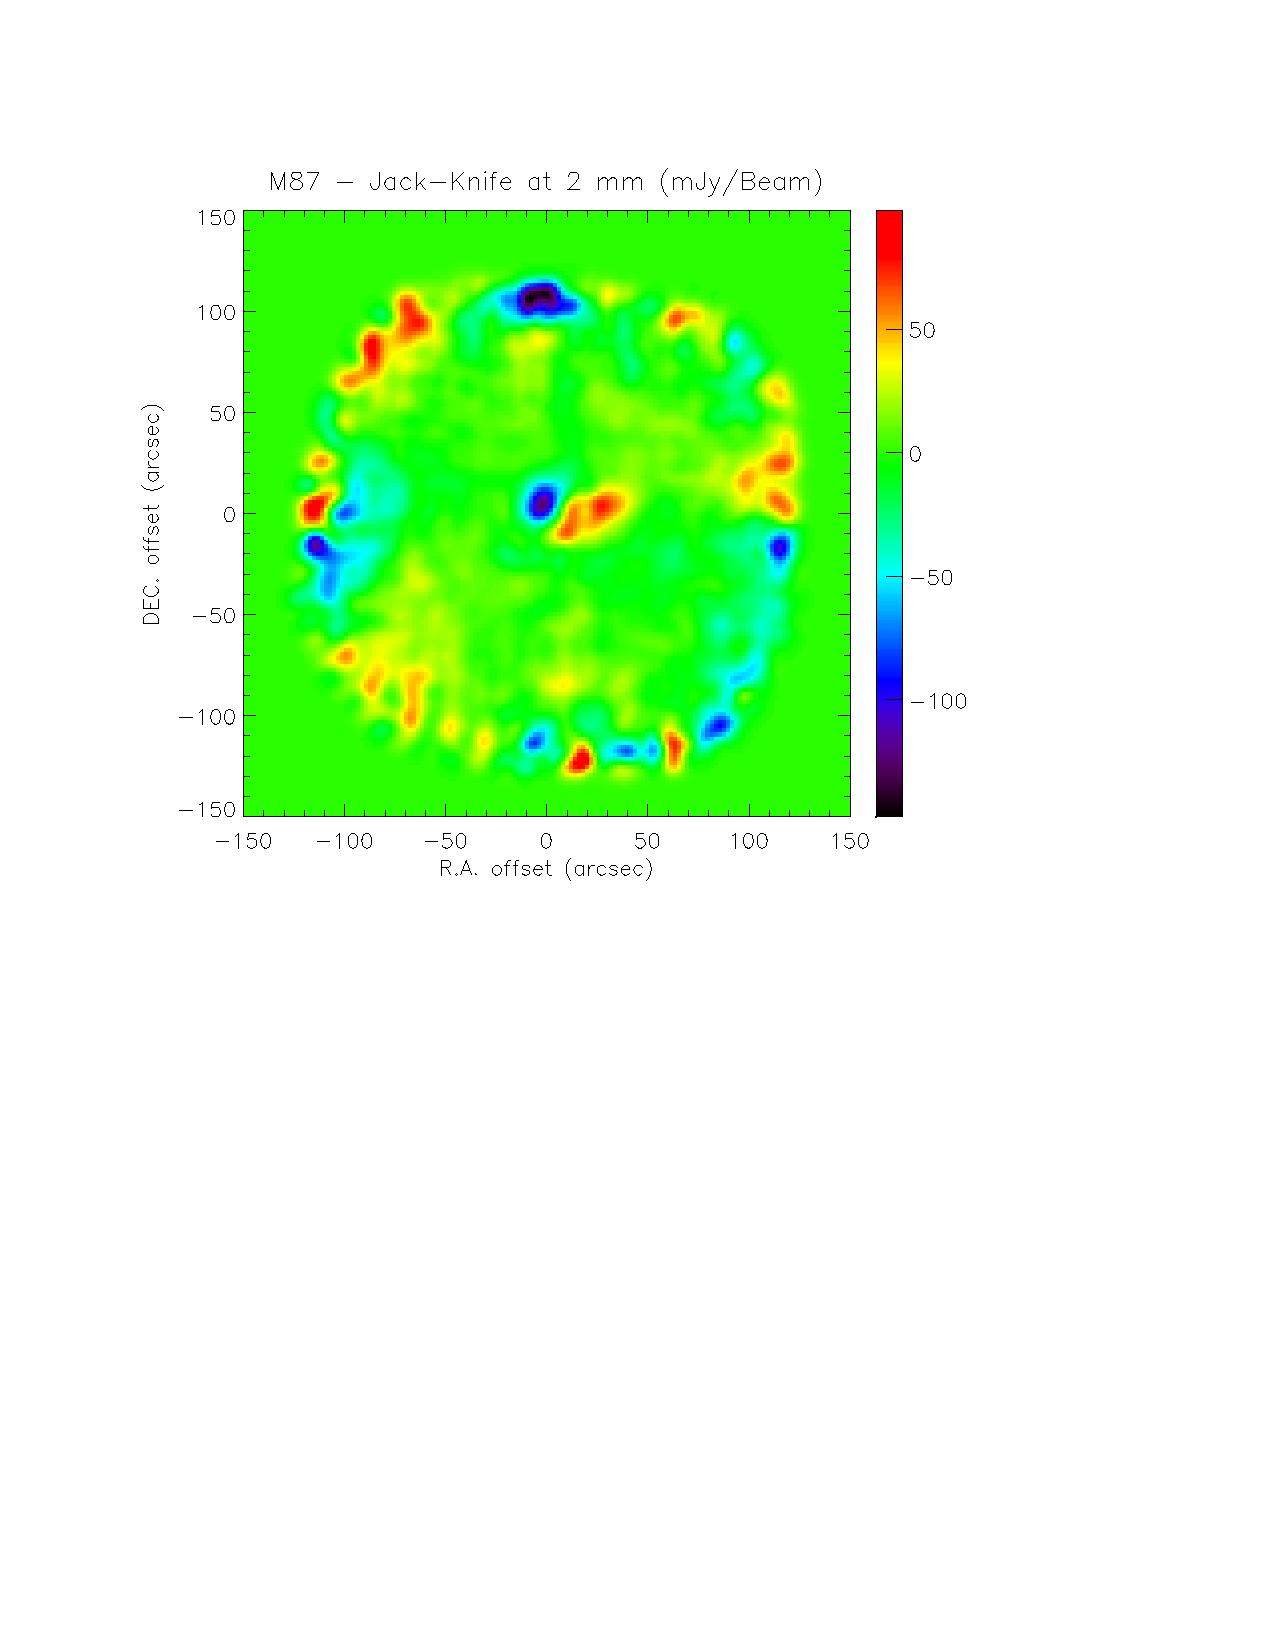
\includegraphics[height=6cm, trim=2cm 13cm 4cm 2cm, clip=true]{Figure/M87_jack-knife_2mm}
\caption{Jack-Knife maps. The residual are not zero because the two sets of map are not strictly equivalent, but it is less than 5\% of the source.}
\label{fig:M87_JK}
\end{figure}

%Profiles
The combined maps allow us to compute the flux profiles of M87 by averaging the flux in concentric annuli. They are given in Fig.~\ref{fig:M87_profile}. The errors propagated form the TOD are shown but they are small compared to the systematics that are not included.
\begin{figure}
\centering
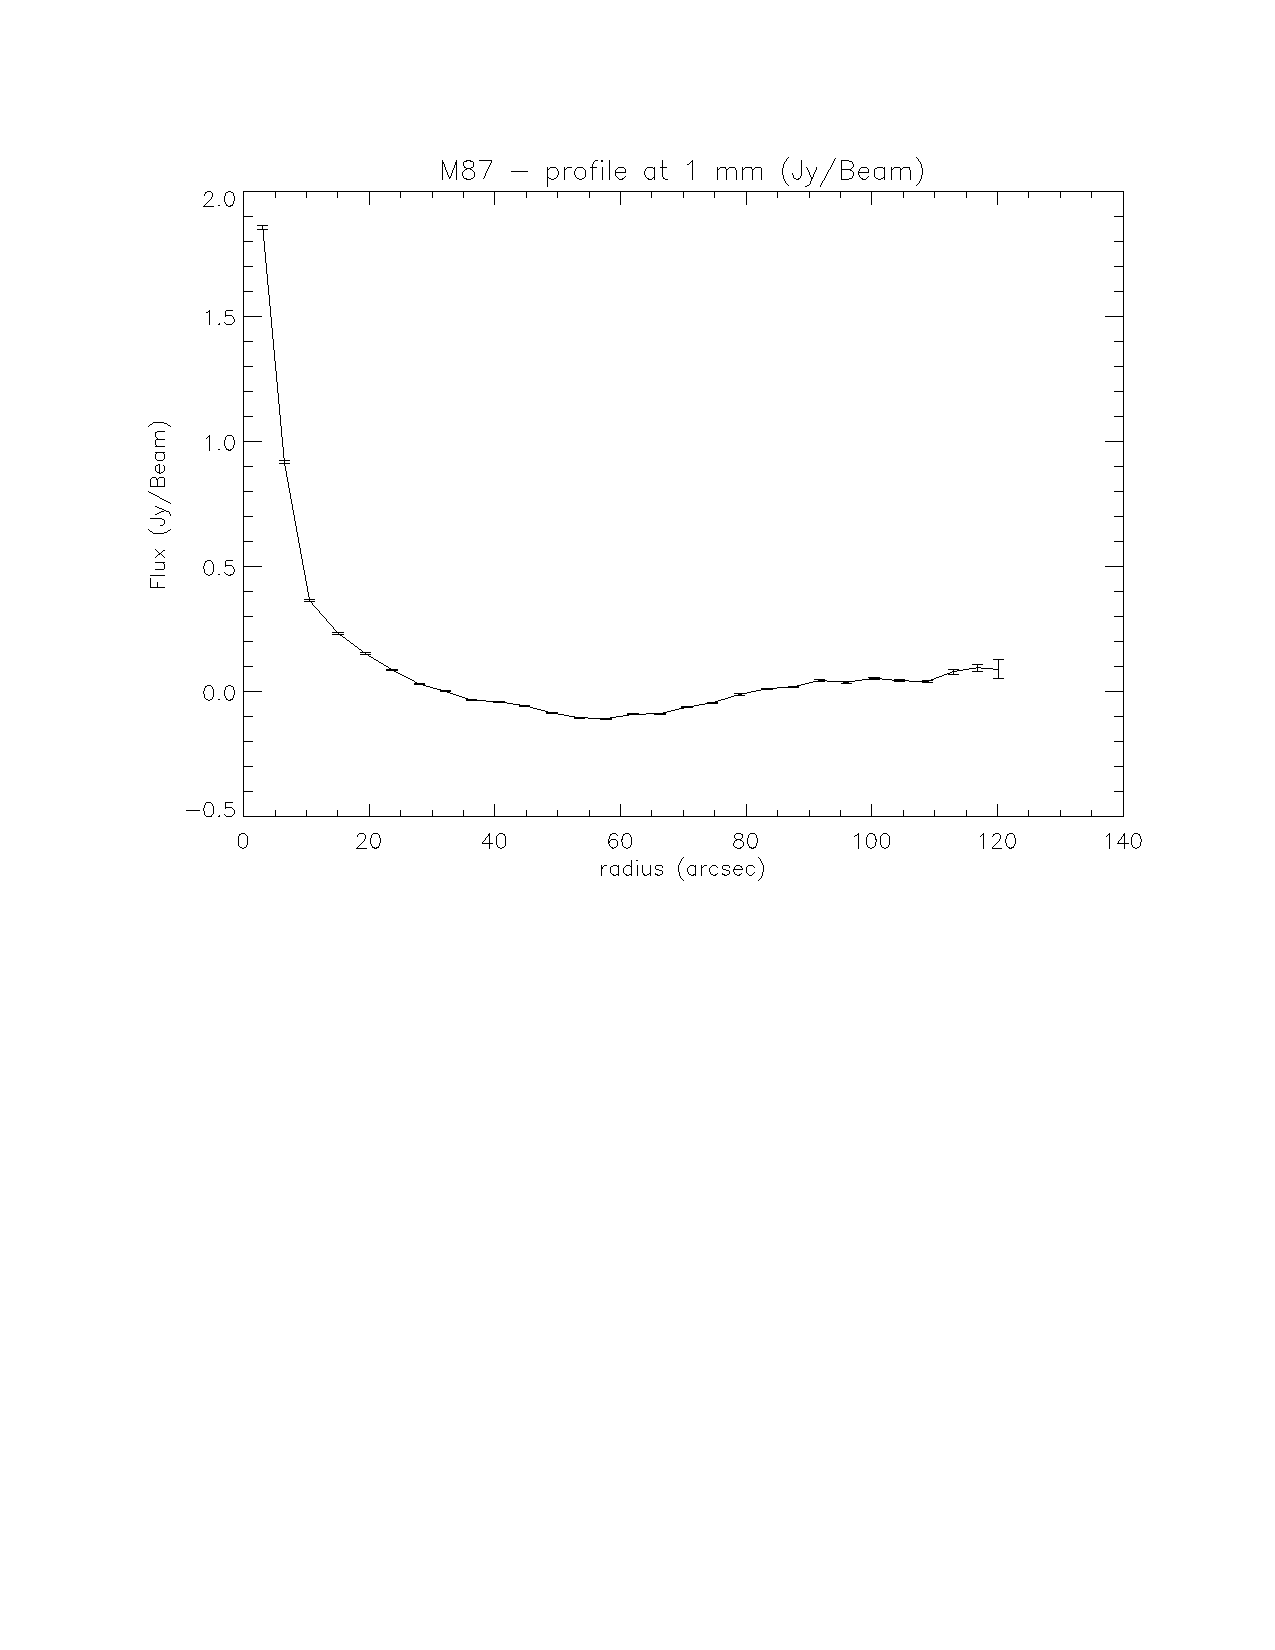
\includegraphics[height=5.5cm, trim=2cm 13cm 2cm 2cm, clip=true]{Figure/M87_profile_1mm}
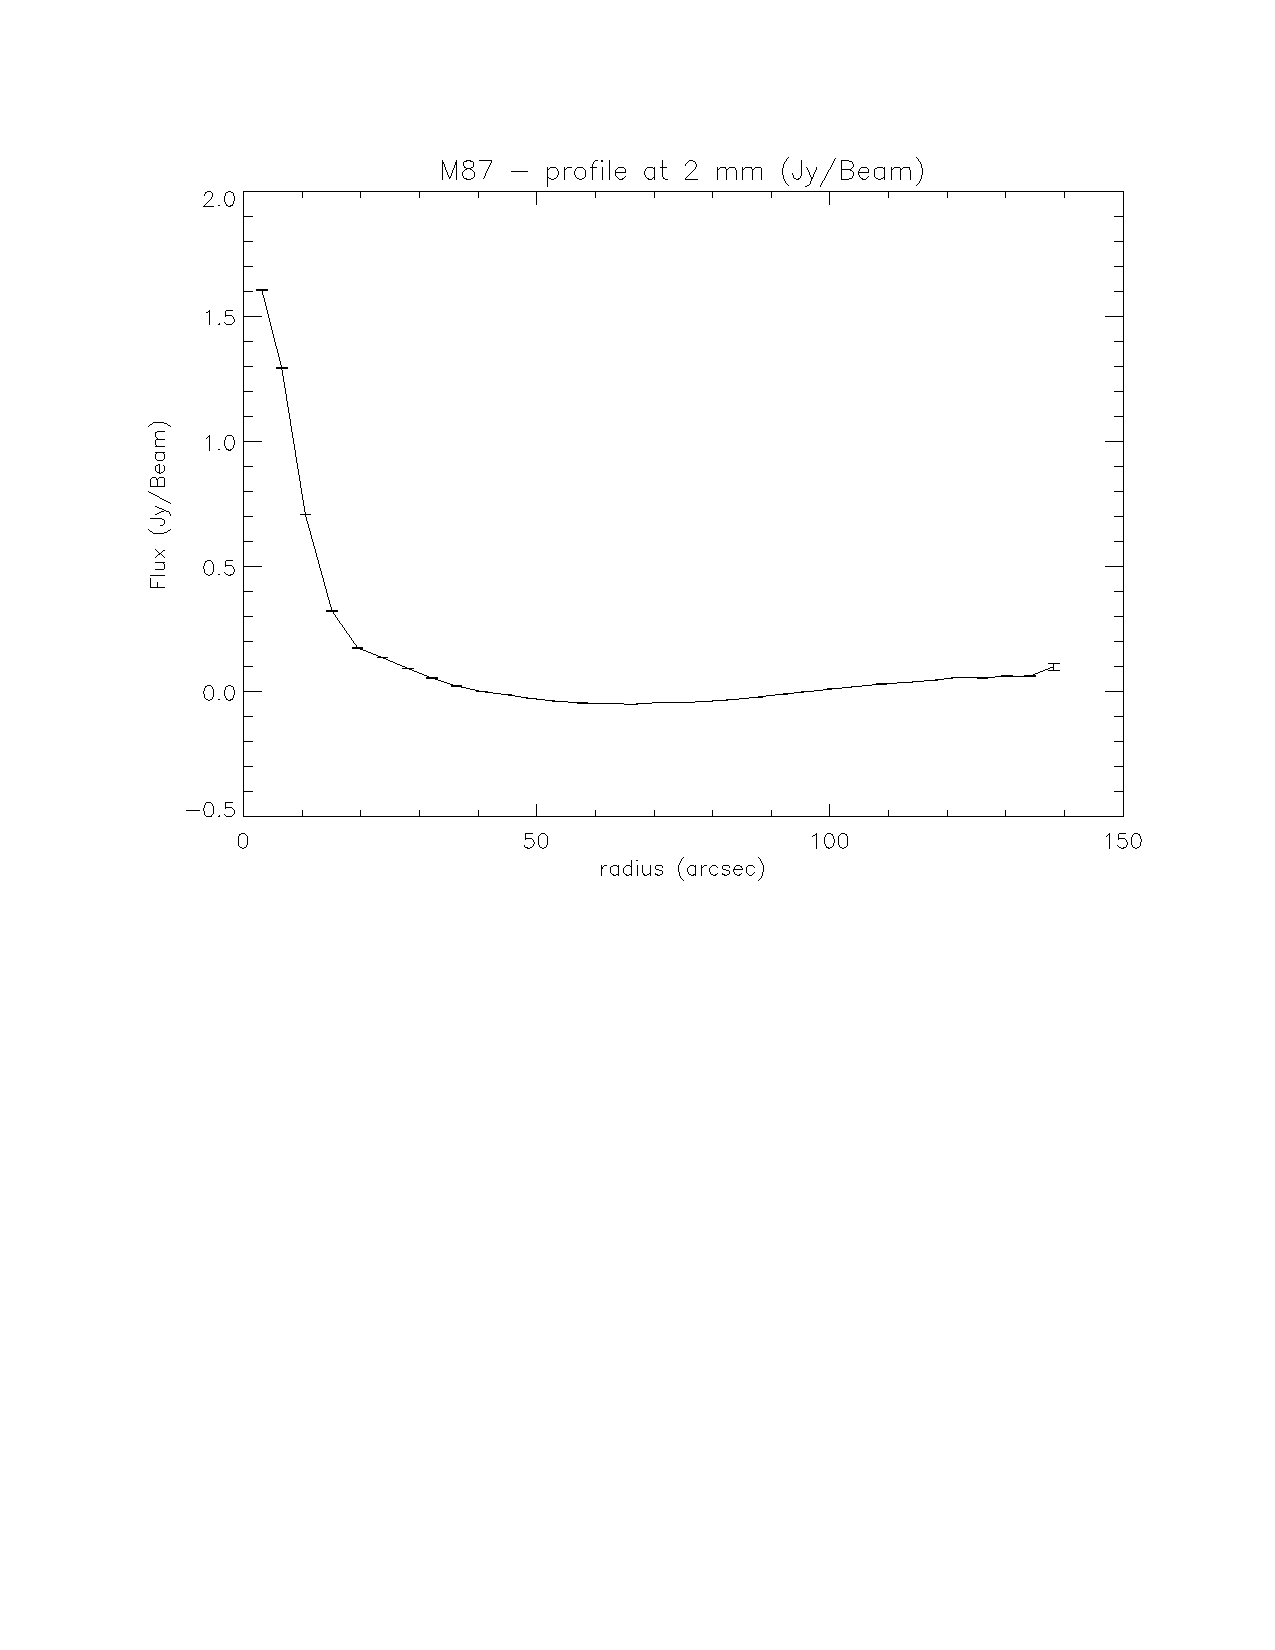
\includegraphics[height=5.5cm, trim=2cm 13cm 2cm 2cm, clip=true]{Figure/M87_profile_2mm}
\caption{Flux profiles of M87 at both wavelength.}
\label{fig:M87_profile}
\end{figure}

%Map per KID
If the keyword {\color{blue} /map\_per\_kid} is set when the pipeline is launched, the individual maps per detectors are computed and combined over the scans. These maps are shown in this example in Fig.~\ref{fig:M87_map_per_KID} for the first four KIDs of the 1mm array. The signal is strong enough to be seen individually.
\begin{figure}
\centering
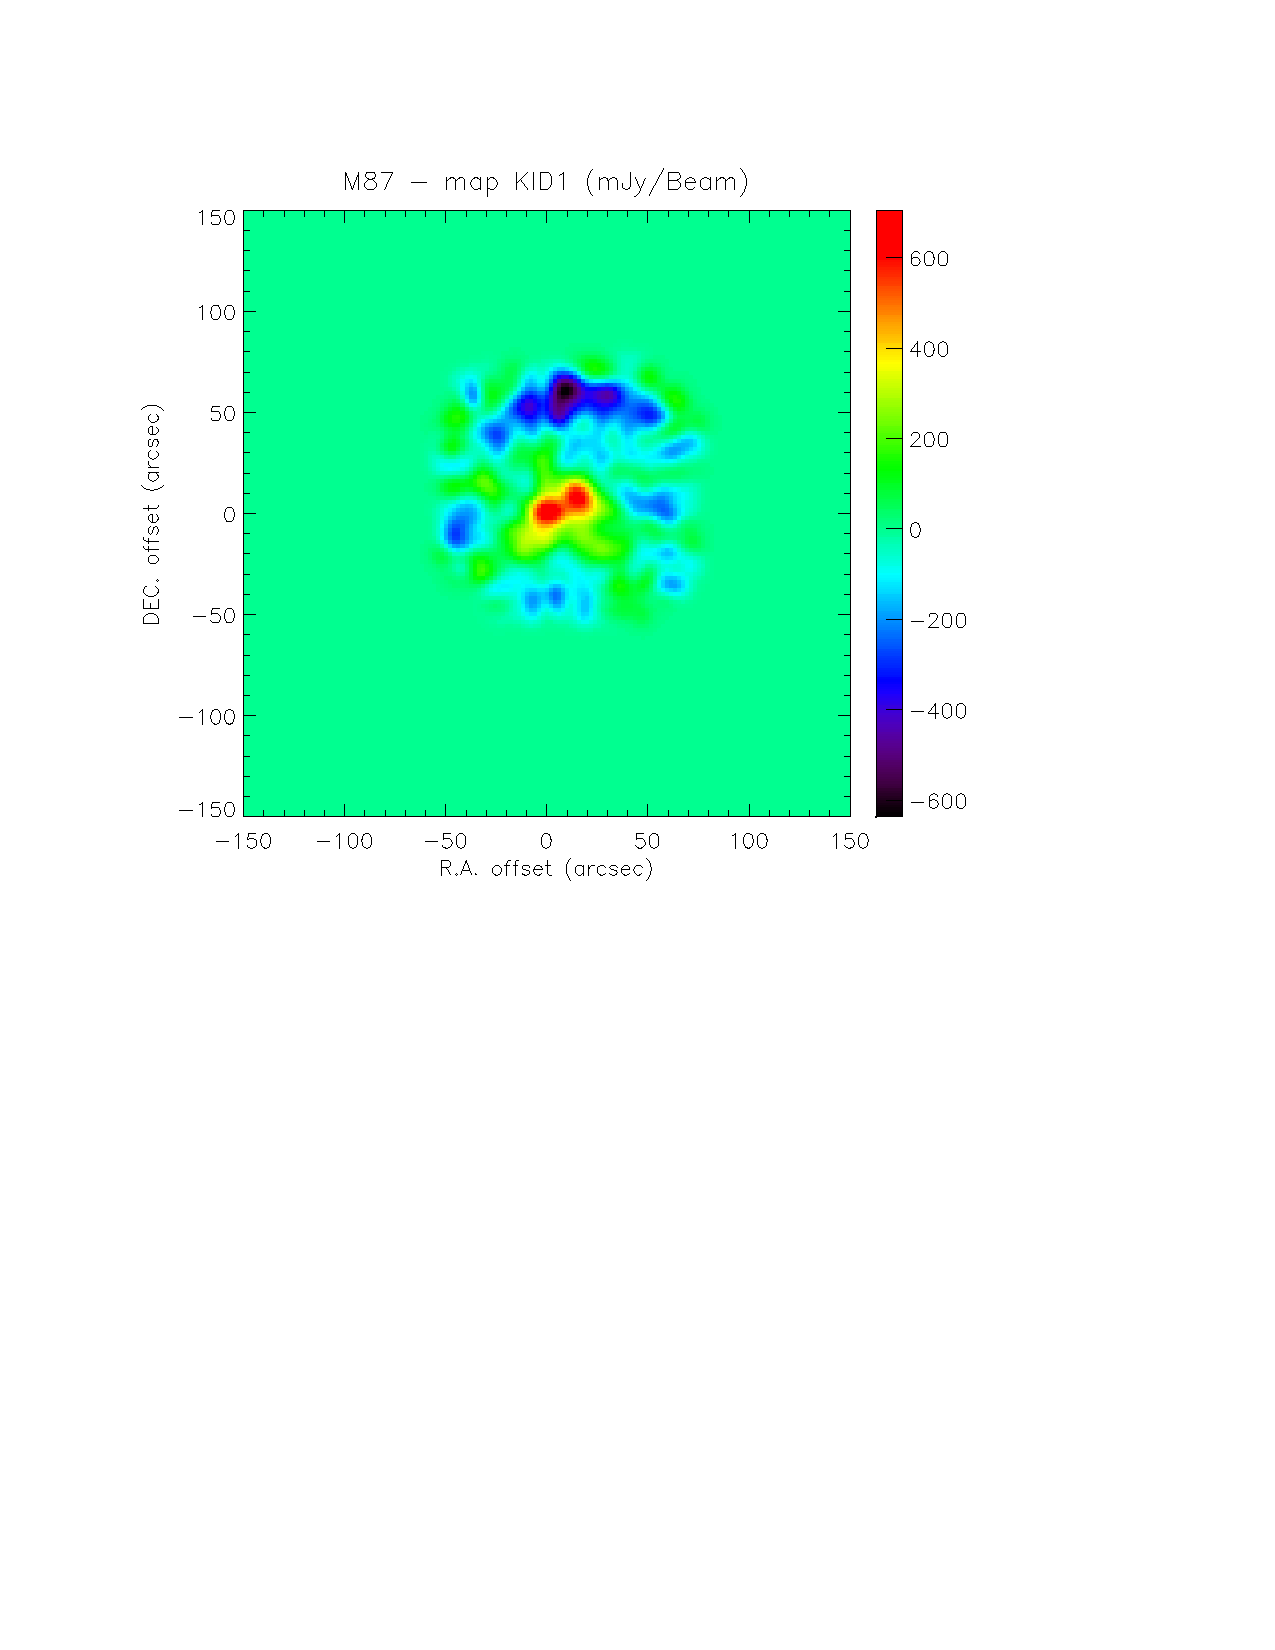
\includegraphics[height=3cm, trim=2cm 13cm 4cm 2cm, clip=true]{Figure/M87_mapKID1}
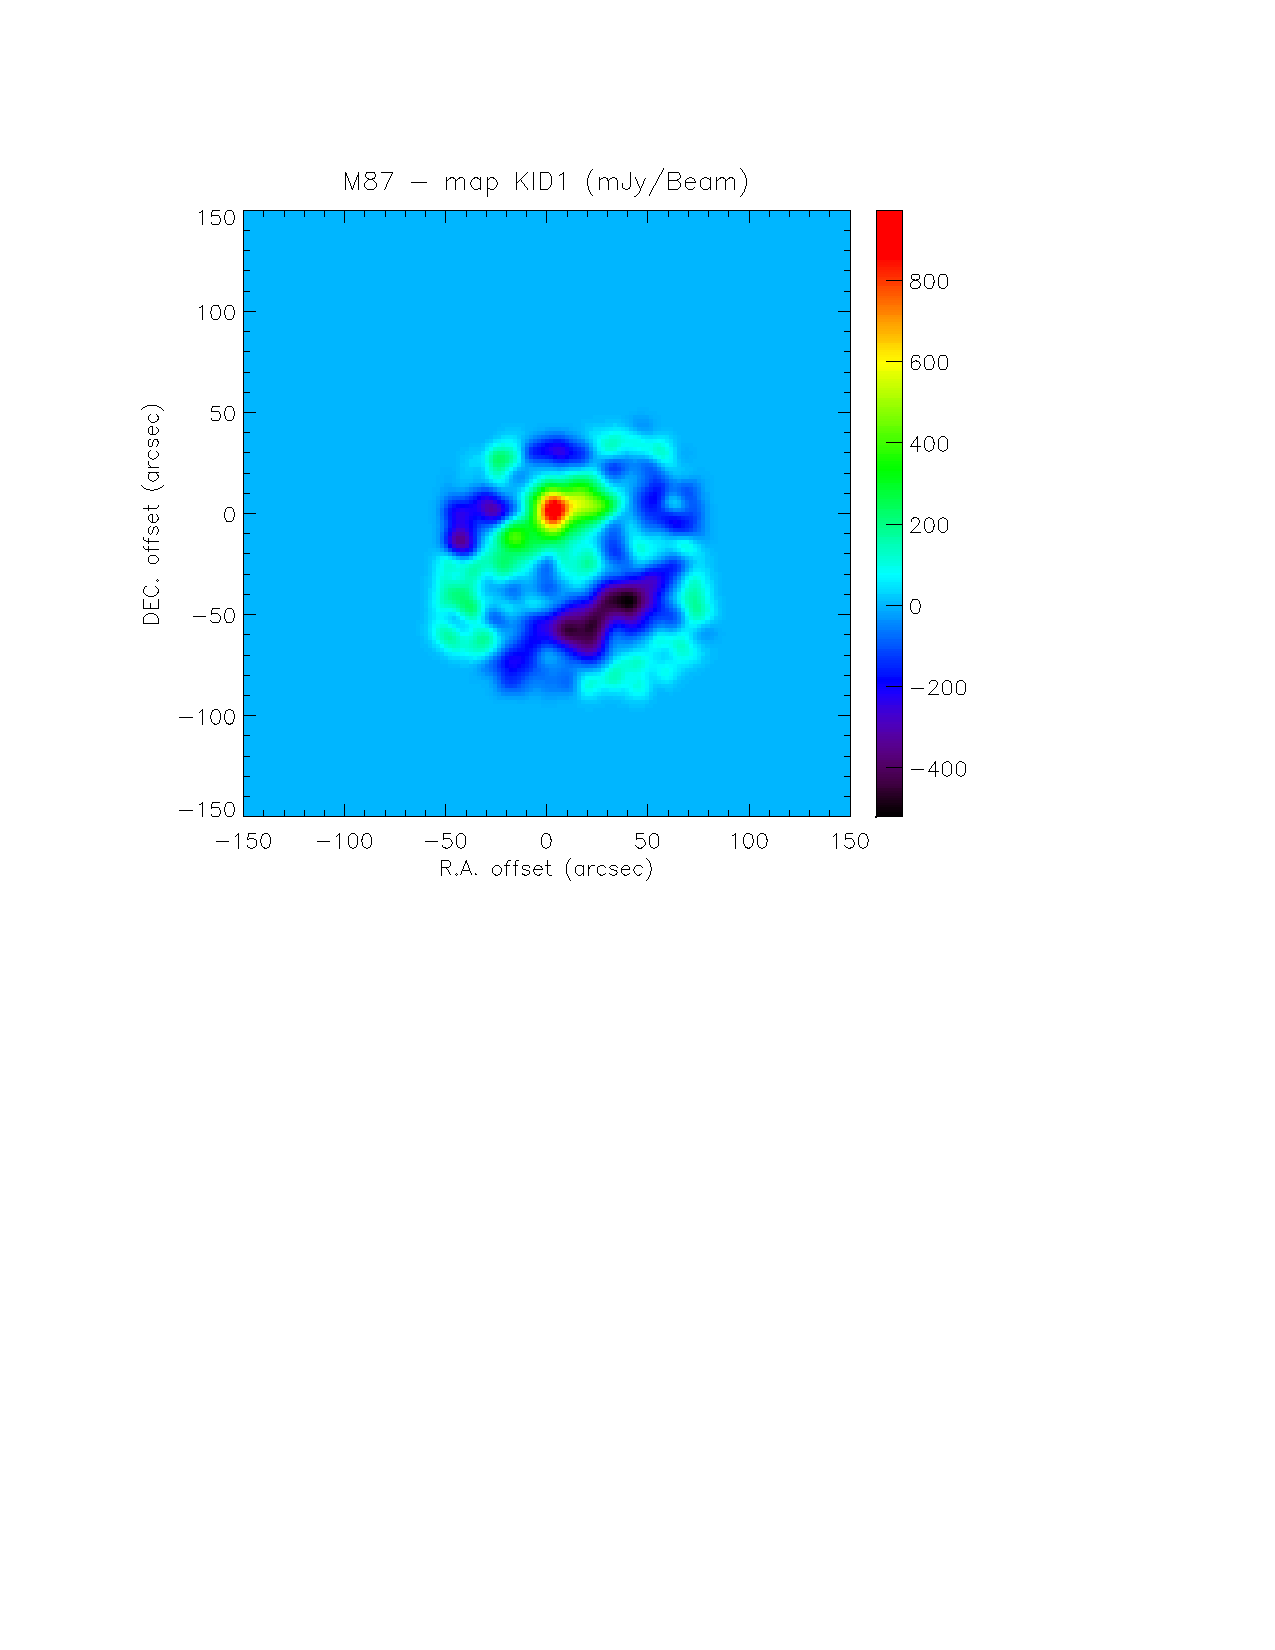
\includegraphics[height=3cm, trim=2cm 13cm 4cm 2cm, clip=true]{Figure/M87_mapKID2}
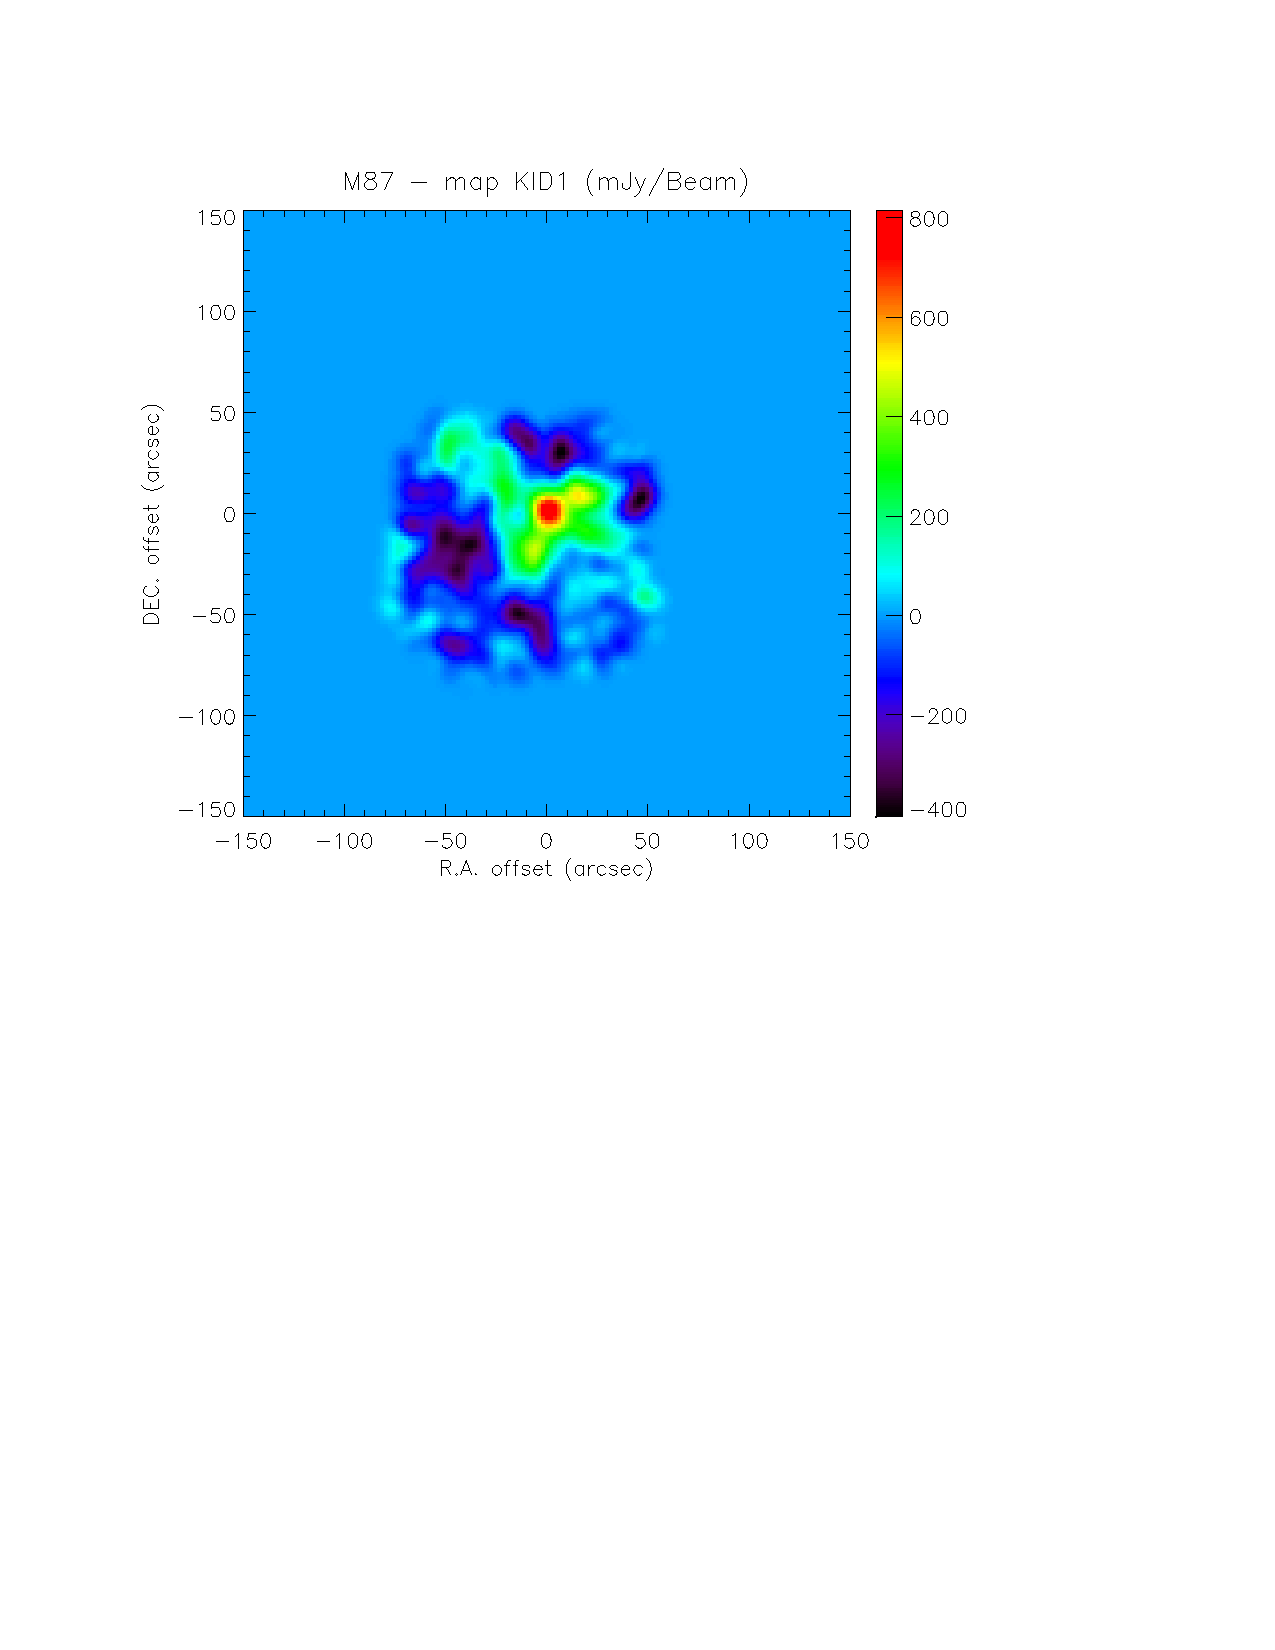
\includegraphics[height=3cm, trim=2cm 13cm 4cm 2cm, clip=true]{Figure/M87_mapKID3}
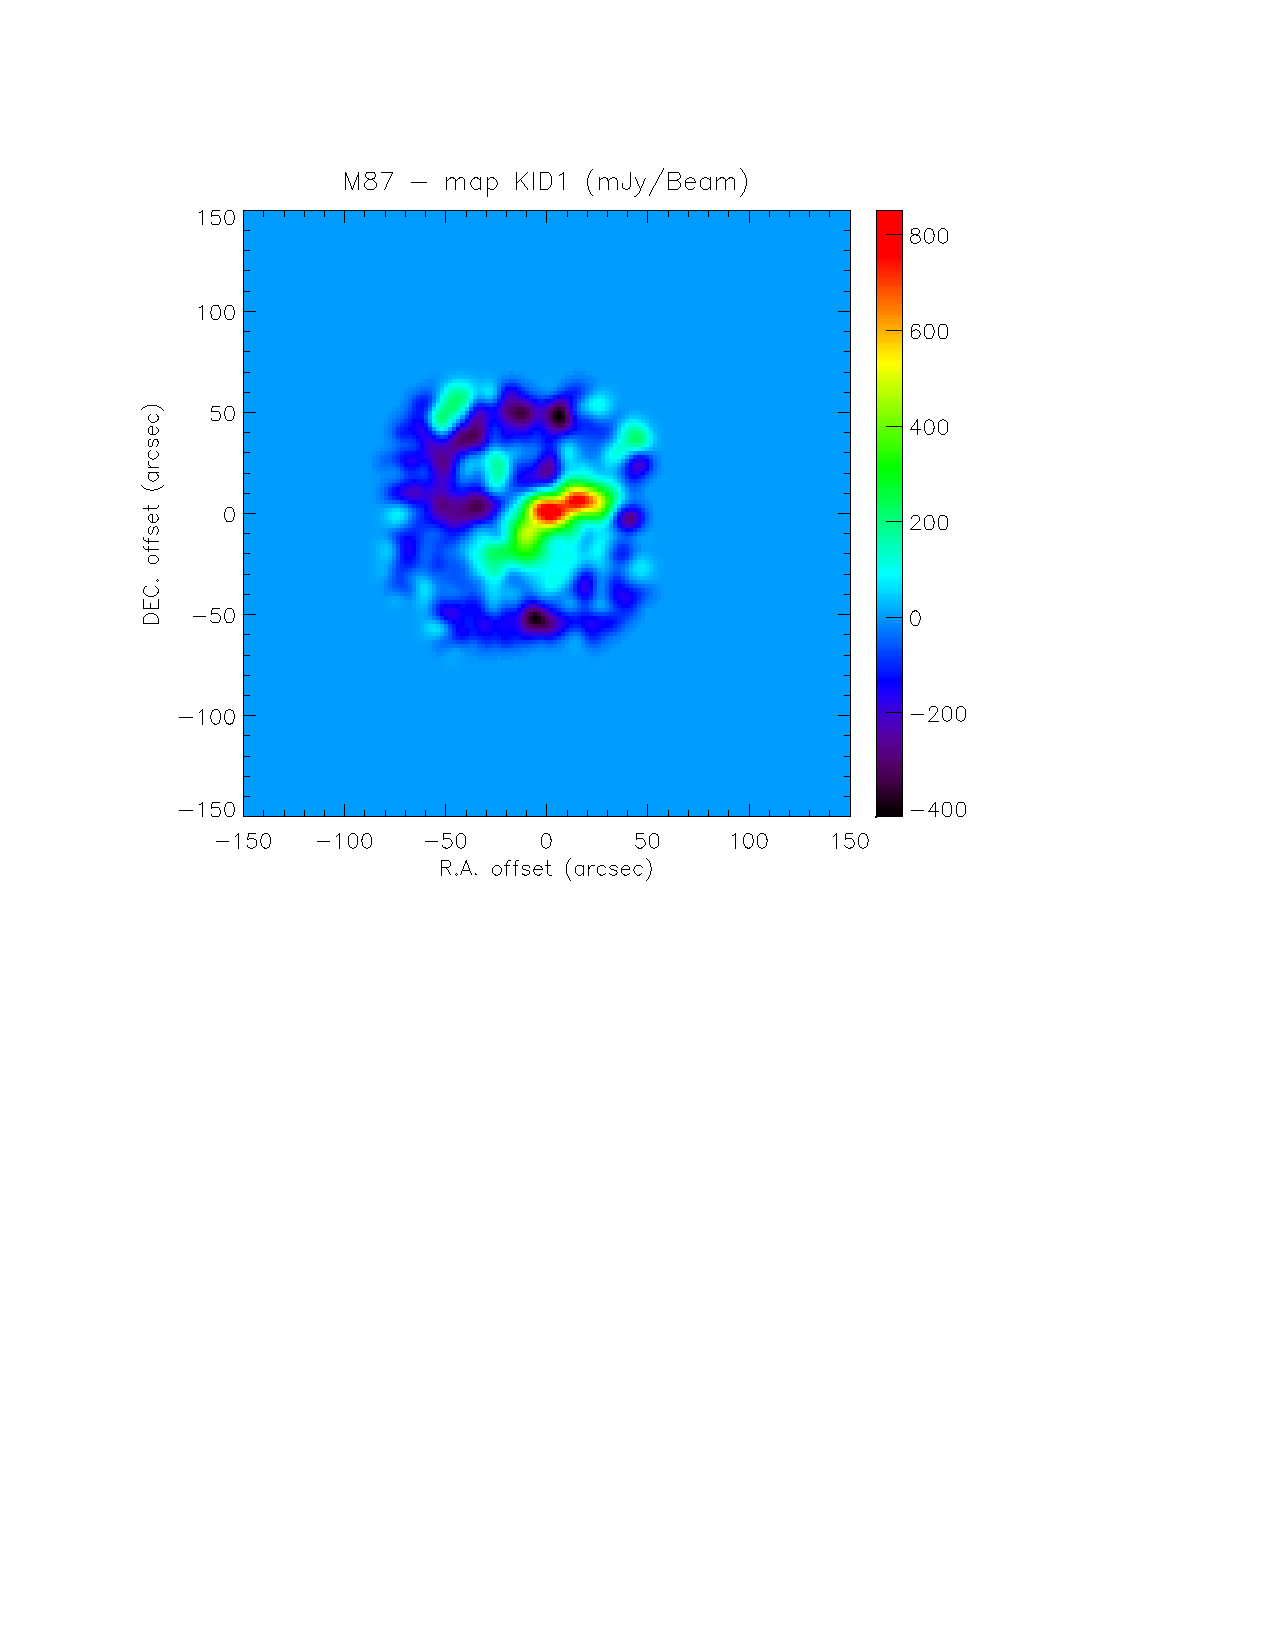
\includegraphics[height=3cm, trim=2cm 13cm 4cm 2cm, clip=true]{Figure/M87_mapKID4}
\caption{Individual KID maps in the case of M87 for the 4 first KIDs of the data structure ({\it i.e.} at 1mm). All scans have been combined here. The maps are noisy but in the case of M87, the source is strong enough to be seen on each map.}
\label{fig:M87_map_per_KID}
\end{figure}

%Nice map
Finally, the flux maps are plotted in Fig.~\ref{fig:M87_nice_map} with the effective beam (instrumental and smoothing), a mask off the region where the noise level is larger than four times the minimum noise level of the map, and given contours.
\begin{figure}
\centering
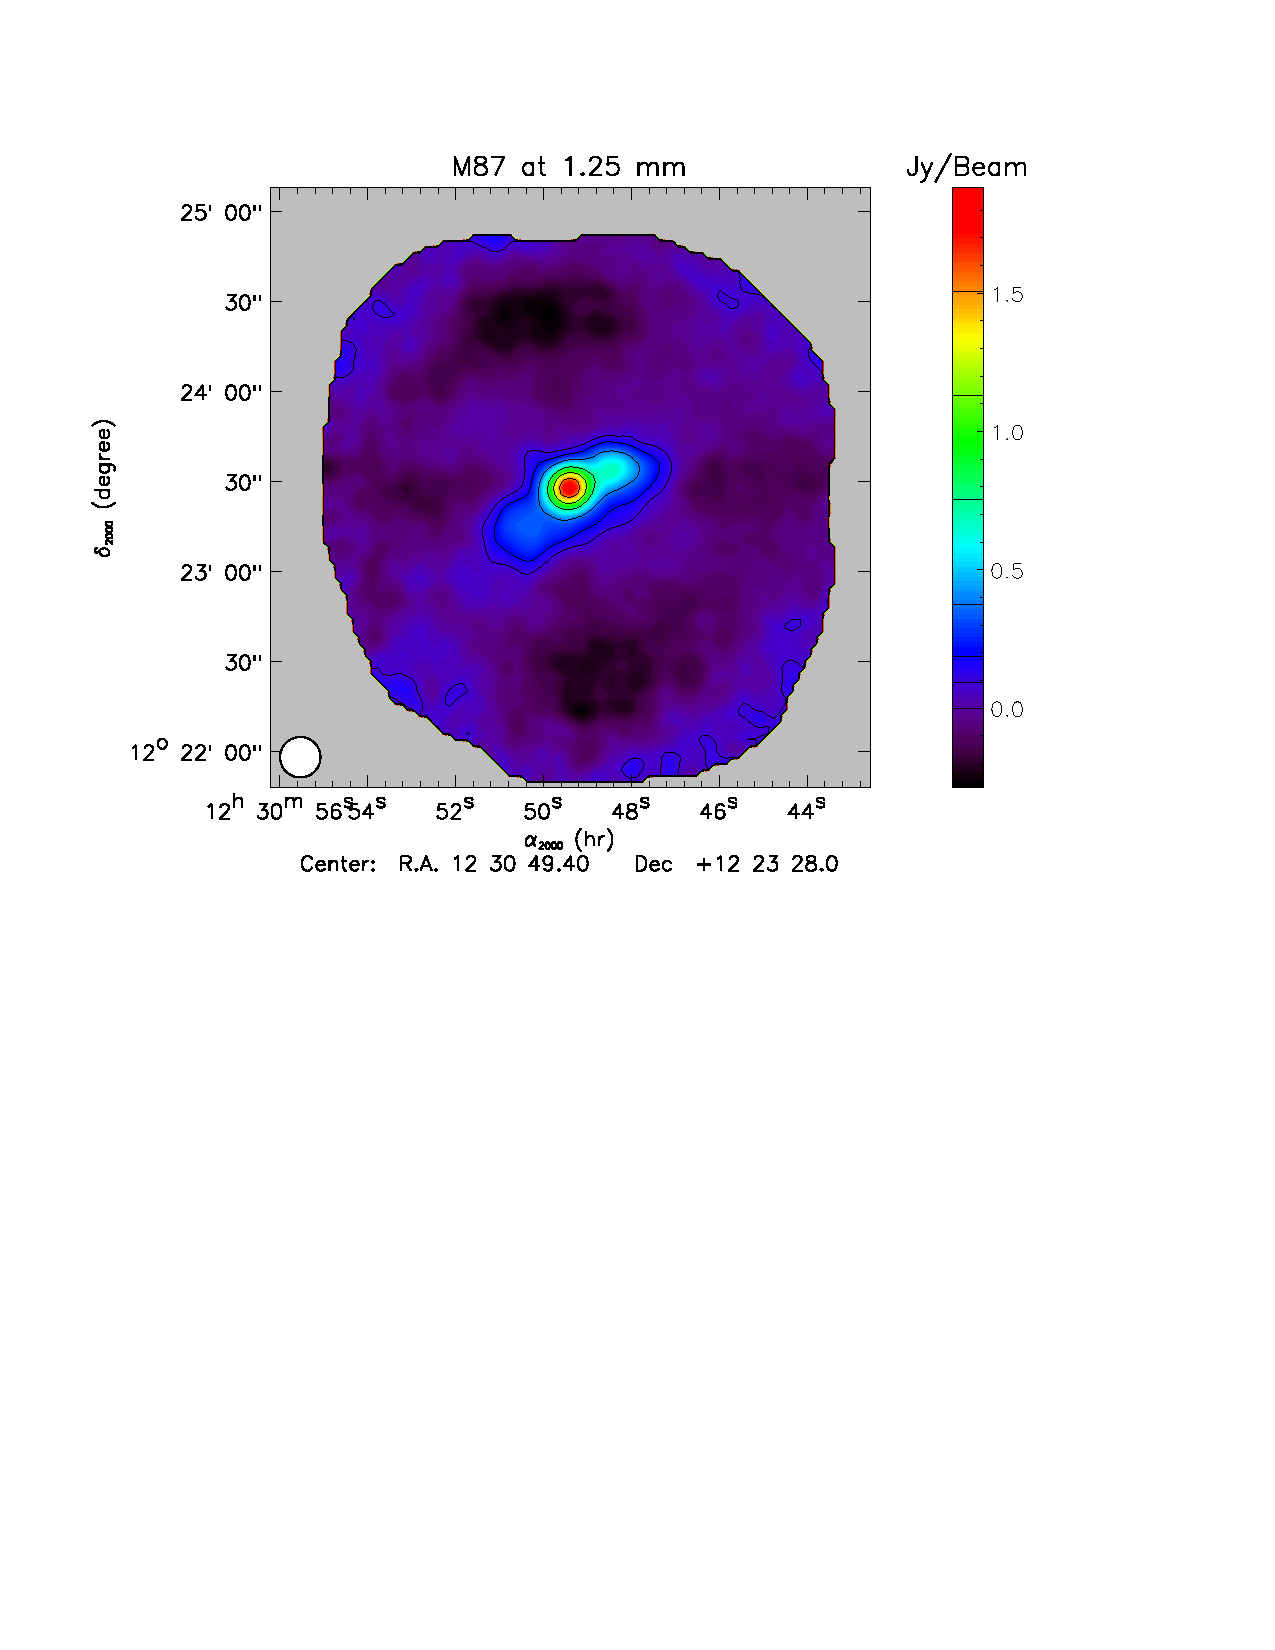
\includegraphics[height=6.0cm, trim=1cm 13cm 4cm 1cm, clip=true]{Figure/M87_1mm}
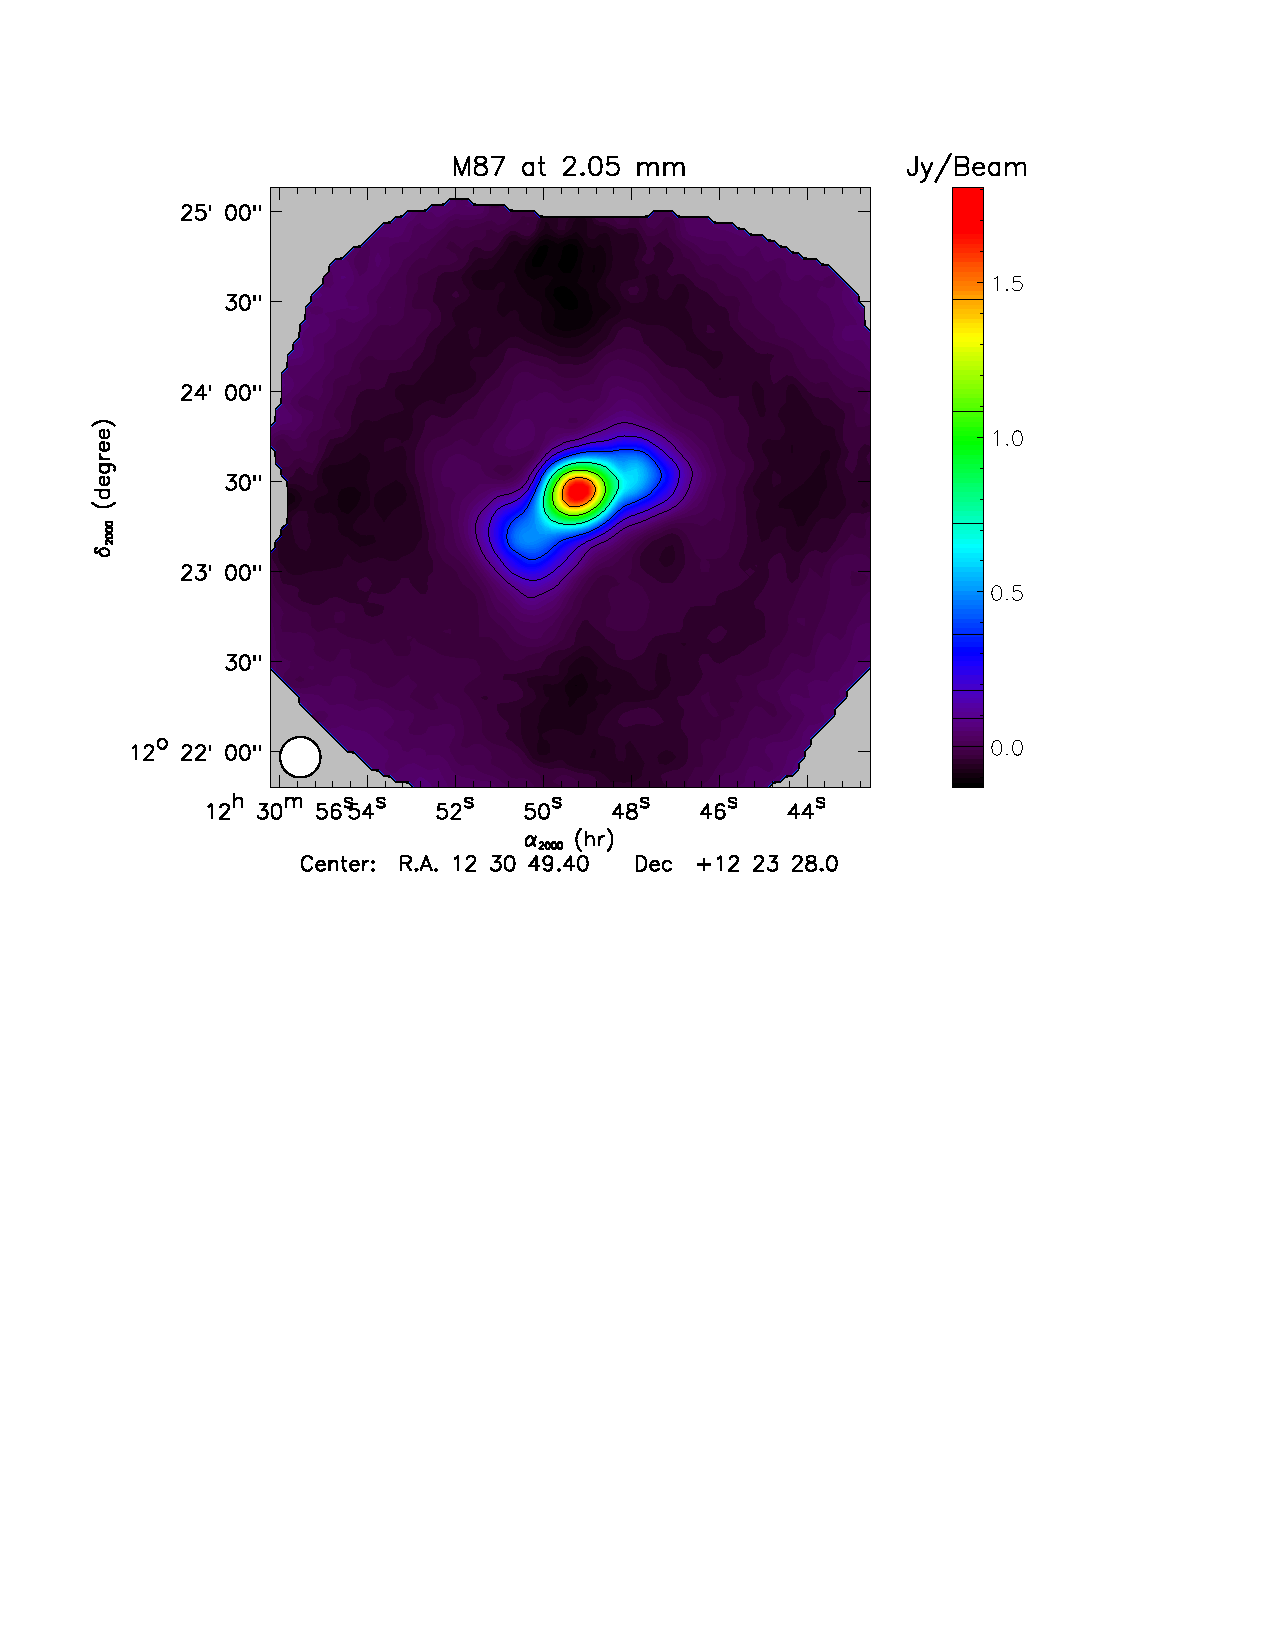
\includegraphics[height=6.0cm, trim=1cm 13cm 4cm 1cm, clip=true]{Figure/M87_2mm}
\caption{Final maps produced at the end of the script for both wavelength in the case of M87. The effective beam FWHM is shown as white circle on the bottom left corner, the map background (or not shown) is set to gray, and black contours are over plotted for clarity.}
\label{fig:M87_nice_map}
\end{figure}

%%%%%%%%%%%%%%%%%%%%%%%%%%%%%%%%%%%%%%%%%%%%%%%%%%%%%%%%%%%%
%%%%%%%%%%%%%%%%%%%%%%%%%%%%%%%%%%%%%%%%%%%%%%%%%%%%%%%%%%%%
\section{Parameters of the pipeline}
\label{sec:param}
This section describes the content of the parameter structure created before launching the pipeline. Tab.~\ref{tab:table_param} resumes this content.
\begin{table}[!h]
	\begin{center}
	\begin{tabular}{cc}
	 \hline
         \hline
	Parameter content & Comment\\
	\hline
	   source & Source name (see Sect.~\ref{sec:info_hand}) \\
           name4file & Name used in saved files (see Sect.~\ref{sec:info_hand}) \\
           version & Version of the analysis (see Sect.~\ref{sec:info_hand}) \\
           coord\_pointing & 	R.A--Dec. pointing coordinates (see Sect.~\ref{sec:info_hand}) \\
           coord\_source & R.A--Dec. coordinates of the source (see Sect.~\ref{sec:info_hand}) \\
           scan\_num & List of the numbers of the scans (see Sect.~\ref{sec:info_hand}) \\
           day & List of the corresponding days (see Sect.~\ref{sec:info_hand}) \\
           scan\_list & List of the scans of the form ['201211s0104', '201211s0105', ...] \\
           kid\_file & KIDs properties file name \\
           config\_file & {\color{red} Nico?}\\
           data\_file & {\color{red} Nico?} \\
           imb\_fits\_file & {\color{red} Nico?} \\
           output\_dir & Directory in which the result files are saved (see Sect.~\ref{sec:info_hand}) \\
           nickname & {\color{red} Nico?} \\
           source\_flux\_jy & Estimated flux of the source in Jy (\{A: flux at 1mm, B: flux at 2mm\}) \\
           map & Substructure described in Sect.~\ref{sec:param_map} \\
           glitch & Substructure described in Sect.~\ref{sec:param_glitch} \\
           decor & Substructure described in Sect.~\ref{sec:param_decor} \\
           filter & Substructure described in Sect.~\ref{sec:param_filter} \\
           w8 & Substructure described in Sect.~\ref{sec:param_w8} \\
           iscan & The index number of the read scan during the loop over all scans \\
           scan\_type & Type of the scan (azimuth or elevation) \\
           tau\_list & List of opacities filled for each scan (\{A: --, B: --\}) \\
           mean\_noise\_list & Idem with the mean standard deviation of the TODs \\
           nu & The central observation frequencies in GHz (\{A: --, B: --\}) \\
           JYperKRJ & Unit conversion computed in the pipeline: Jy/K$_{\mathrm{RJ}}$ \\
           KRJperKCMB & Unit conversion computed in the pipeline: K$_{\mathrm{RJ}}$/K$_{\mathrm{CMB}}$ \\
           KCMBperY & Unit conversion computed in the pipeline K$_{\mathrm{CMB}}$/y$_{\mathrm{Compton}}$ \\
	\hline
	\end{tabular}
	\end{center}
	\caption{Content of the parameter structure}
	\label{tab:table_param}
	\end{table}

\subsection{The param.map substructure }
\label{sec:param_map}
This substructure contains the resolution in {\color{blue} param.map.reso} and the size of the map along the right ascension and the declination in {\color{blue} param.map.size\_\{ra, dec\}}, given in arcsec.

\subsection{The param.glitch substructure }
\label{sec:param_glitch}
This contains the deglitching parameters such as the number of points over which we look for glitches in {\color{blue} param.glitch.width} and the number of $\sigma$ above which they are flagged in {\color{blue} param.glitch.nsigma}.

\subsection{The param.decor substructure }
\label{sec:param_decor}
This substructure contains the parameters associated to the decorrelation methods described in Sect.~\ref{sec:decor_methods}. It can be resumed as follow:
\begin{itemize}
\item {\color{blue} param.decor.IQ\_plane}
	\begin{itemize}
	\item {\color{blue} .apply}: set to 'yes' (resp. 'no') if you want to decorrelate the electronic noise in the $I-Q$ plane
	\item {\color{blue} .per\_subscan}: set to 'yes' (resp. 'no') if you want to do the decorrelation per subscan (resp. the full scan)
	\item {\color{blue} .one\_mode}: set to 'yes' if you want to combined the OFFs tones in one common mode and to 'no' if you want to use them all separately 
	\end{itemize}
	\item {\color{blue} param.decor.method}: this parameter give the name of the decorrelation method used. See Sect.~\ref{sec:decor_methods} to check the possible names.
\item {\color{blue} param.decor.median}
	\begin{itemize}
	\item {\color{blue} .width}: contains the width in number of points of the median filter.
	\end{itemize}
\item {\color{blue} param.decor.source\_interpol} 
	\begin{itemize}
	\item {\color{blue} .d\_min}: contains the limit distance below which we consider to be on the source
	\end{itemize}
\item {\color{blue} param.decor.common\_mode}
	\begin{itemize}
	\item {\color{blue} per\_subscan}: set to 'yes' (resp. 'no') if you want to do the decorrelation per subscan (resp. the full scan)
        \item {\color{blue} x\_calib}: set to 'yes' (resp. 'no') if you want to cross calibrate the atmosphere
        \item {\color{blue} nsmooth}: Number of points over which the common mode is smoothed
	\item {\color{blue} d\_min}: Give the limit distance above which we consider a KID to be far in the focal plane (from the KID that we are decorrelating)
	\end{itemize}
\item {\color{blue} param.decor.dual\_band}
	\begin{itemize}
	\item {\color{blue} per\_subscan}: set to 'yes' (resp. 'no') if you want to do the decorrelation per subscan (resp. the full scan)
        \item {\color{blue} x\_calib}: set to 'yes' (resp. 'no') if you want to cross calibrate the atmosphere
        \item {\color{blue} nsmooth\_temp}: Number of points over which the common mode is smoothed
        \item {\color{blue} fcut}: Give the low frequency limits of the cosine squared cutoff in Hz ({\it e.g.} [1.5, 2.0])
	\end{itemize}
\item {\color{blue} param.decor.full}
	\begin{itemize}
	\item {\color{blue} per\_subscan}: set to 'yes' (resp. 'no') if you want to do the decorrelation per subscan (resp. the full scan)
	\end{itemize}
\end{itemize}

\subsection{The param.filter substructure }
\label{sec:param_filter}
This substructure contains the filtering parameters. They are as follow:
\begin{itemize}
 \item {\color{blue} param.map.filter.apply}: 'yes' or 'no' depending if you want to apply the filter
 \item {\color{blue} param.map.filter.width}: the number of points considered when the pulse tube lines are flagged
 \item {\color{blue} param.map.filter.nsigma}: number of $\sigma$ above which the lines are flagged
 \item {\color{blue} param.map.filter.freq\_start}: frequency at which the search for lines starts
 \item {\color{blue} param.map.filter.low\_cut}: the data are low frequency cut. This gives the two frequencies between which the cosine cutoff is progressively applied in Hz ({\it e.g.} [0.03, 0.04])
 \item {\color{blue} param.map.filter.cos\_sin}: Set to 'yes' if you want to apply cosine and sine filtering of low frequencies
\end{itemize}

\subsection{The param.w8 substructure }
\label{sec:param_w8}
This contains the limit distance, in arcsec, for considering a given detector to be on source in {\color{blue} param.w8.dist\_off\_source} (on source parts of the TODs are not used for computing the weights) and specify if the weight are given per subscan or for all the scan in {\color{blue} param.w8.per\_subscan} ('yes' or 'no').

%%%%%%%%%%%%%%%%%%%%%%%%%%%%%%%%%%%%%%%%%%%%%%%%%%%%%%%%%%%%
%%%%%%%%%%%%%%%%%%%%%%%%%%%%%%%%%%%%%%%%%%%%%%%%%%%%%%%%%%%%

\section{Modules description}
\label{sec:module_description}
All the modules of the {\it NIKA} pipeline can be found under the directory {\color{blue} your\_SVN\_path/Pipeline/Run6/}. They all start by {\color{blue} nika\_pipe}. This section gives an overview of the content of each module.

\subsection{{\color{blue}nika\_pipe\_launch.pro}}
\label{sec:nika_pipe_launch}
This is the main module of the pipeline. It does not compute anything but launches all the sub-modules one after the other for each scan required in the parameter structure. Once all the individual maps are computed, they are combined and saved with the appropriate astrometry. If required, the individual scan maps and the maps per detector are also saved.

\subsubsection*{Calling sequence}
{\color{blue} nika\_pipe\_launch, param, map\_combi, map\_list}\\
where the param structure should be such as described in Sect.~\ref{sec:param}. The module always returns the combined map (map\_combi) and the maps per scan (map\_list). They are structures which contain the following fields
\begin{itemize}
\item {\color{blue} A}: substructure concerning the 1mm channel
\begin{itemize}
\item {\color{blue} Jy}: flux map in Jy/Beam.
\item {\color{blue} var}: variance map, in (Jy/Beam)$^2$ estimated from the error propagation using the TODs
\item {\color{blue} time}: the time per pixel map in seconds.
\end{itemize}
\item {\color{blue} B}: substructure concerning the 2mm channel with similar sub-substructures.
\end{itemize}
\subsubsection*{Keywords} 
\begin{itemize}
\item {\color{blue} /save}: set this keyword to save the maps produced.
\item {\color{blue} /map\_per\_kid}: set this keyword if you want to compute a map per detector.
\item {\color{blue} /ps}: produce postscript intermediate plots instead of showing them online.
\item {\color{blue} /png}: idem with png plots (both keywords are compatible)
\item {\color{blue} add\_source=add\_source}: add a source by hand in the TOD (see the module nika\_pipe\_addsource.pro for further details)
\item {\color{blue} /simu}: set this keyword if you analyze simulated data (see Sect.~\ref{sec:simu} for further details)
\item {\color{blue} kidlist=kidlist}: give the list of KIDs to be used. All the KIDs are used by default.
\item {\color{blue} /logbook}
\end{itemize}

\subsection{{\color{blue} nika\_pipe\_getdata.pro}}
Get the data in the structure called data and the KID parameters in the structure called kidpar for the given scan known from the input parameter structure. The data are read using external calls of C++ codes so that the user should compile them before using it (by launching {\color{blue} compile\_read\_nika}). The raw data files should be in the directory {\color{blue} !nika.RAW\_ACQ\_DIR}. The data that are read by default are as follows:
\begin{itemize}
\item {\color{blue} subscan}
\item {\color{blue} scan}
\item {\color{blue} el}
\item {\color{blue} RF\_didq}
\item {\color{blue} retard 49}
\item {\color{blue} ofs\_az}
\item {\color{blue} ofs\_el}
\item {\color{blue} paral}
\item {\color{blue} scan\_st} 
\item {\color{blue} F\_TONE}
\item {\color{blue} DF\_TONE}
\end{itemize}
Finally, the unit conversion coefficients are computed taking into account the bandpasses.

\subsection{{\color{blue} nika\_pipe\_opacity.pro}}
Compute the zenithal opacity from skydips. {\color{red} Andrea, do you want to add something?}

\subsection{{\color{blue} nika\_pipe\_calib.pro}}
Calibrate the data from Hz (RFdIdQ) to Jy using the KID parameter kidpar.calib that has been computed from planets. The opacity correction is applied here and take into account the elevation of the source.

\subsection{{\color{blue} nika\_pipe\_addsource.pro}}
\label{sec:nika_pipe_addsource}
This procedure allows you to add a source by hand in the TODs. In this case the pipeline ({\color{blue} nika\_pipe\_launch}) should be used with the keyword {\color{blue} add\_source=add\_source}, a structure that give the parameters of the simulated source. The possible kind of sources are as follow 
\begin{itemize}
\item A point source, {\it e.g.} \\
{\color{blue} add\_source = \{type: 'point\_source', flux\_a: 2.0, flux\_b: 1.0, pos: [20.0, 40.0]\}}
\item A SZ cluster, {\it e.g.} \\
{\color{blue} add\_source = \{type: 'cluster', z:0.45, M\_500: 0, P0: 526e-12, a: 0.9, b: 5.0, c: 0.0, rs: 406.0, pos: [0.0, 0.0]\}}
\item A SZ cluster containing a point source, {\it e.g.} \\
{\color{blue} add\_source = \{type: 'cluster+ps', \$ \\
 cluster: \{z: 0.45, M\_500: 0, P0: 526e-12, a: 0.9, b: 5.0, c: 0.0, rs: 406.0, pos: [0.0, 0.0]\}, \$ \\
 ps: \{flux\_a: 3e-3, flux\_b: 4e-3, pos: [20.0, 60.0]\}\}}
\item A sharp disk, {\it e.g.} \\
{\color{blue} add\_source = \{type: 'disk', radius: 30.0, flux\_a: 2.0, flux\_b: 1.0, pos: [20.0, 40.0]\}}
\end{itemize}
Where {\color{blue} pos} give the position of the source with respect to the pointing, in arcsec. The fluxes are all in Jy. Note that here the mass {\color{blue} M\_500} is set to 0 because the simulation of the clusters is done using the normalization {\color{blue} P0} (in Pa) and not the scaling law that requires the mass to compute the pressure. If the mass is non zero, then {\color{blue} P0} becomes a unitless normalization and the pressure is computed from the $\Lambda$CDM cosmological model. 

\subsection{{\color{blue} nika\_pipe\_deglitch.pro}}
This module deglitch the data by flagging peaks above the noise after having removed a baseline. The TODs are interpolated at the giltches locations. Note that in the case of an $I-Q$ plane decorrelation of the electronic noise, the glitches are flagged in the $I$, $Q$, $dI$, $dQ$ TODs.

\subsection{{\color{blue} nika\_pipe\_jump.pro}}
This module does not exist yet. When written, it should correct the jumps that are present in the TODs.

\subsection{{\color{blue} nika\_pipe\_flagkid.pro}}
Procedure that flag bad detectors according to their statistical properties. For now, it is far from being usable correctly.

\subsection{{\color{blue} nika\_pipe\_decor.pro}}
\label{sec:decor_methods}
Decorrelates the noise from the data using the required method in the parameter structure. The possible methods (so far) are
\begin{itemize}
\item {\color{blue} nika\_pipe\_iqdec.pro}: This procedure decorrelates the electronic noise in the $I-Q$ plane using the OFF resonance tones. For this, all the resonances are rotated and normalized to be comparable. RFdIdQ is then computed once the TODs $I$, $Q$, $dI$ and $dQ$ are clean. The calibration is also re-applied. Note that this module in addition to the others.
\item You can choose to use no decorrelation \\
({\color{blue} param.decor.method = 'NONE'})
\item {\color{blue} nika\_pipe\_median\_simple\_dec.pro}: Uses a simple median filter of the data \\
({\color{blue} param.decor.method = 'MEDIAN\_SIMPLE'})
\item {\color{blue} nika\_pipe\_mediandec.pro}: Uses a simple median filter to flag the source and reiterates with the source masked \\
({\color{blue} param.decor.method = 'MEDIAN'})
\item {\color{blue} nika\_pipe\_interpol\_source.pro}: Remove a template of the atmosphere which is simply the TOD interpolated at the source location \\
({\color{blue} param.decor.method = 'SOURCE\_INTERPOL'})
\item {\color{blue} nika\_pipe\_cmdec.pro}: Build a common mode that is template fitted and removed from each TOD \\
({\color{blue} param.decor.method = 'COMMON\_MODE'})
\item {\color{blue} nika\_pipe\_cmkidfar.pro}: Remove a common mode built from the KIDs that are far in the focal plane from the considered detector\\
({\color{blue} param.decor.method = 'COMMON\_MODE\_KIDS\_FAR'})
\item {\color{blue} nika\_pipe\_cmkidout.pro}: Remove a common mode built from the KIDs that are off the source\\
({\color{blue} param.decor.method = 'COMMON\_MODE\_KIDS\_OUT'})
\item {\color{blue} nika\_pipe\_cmgaussfit.pro}: Build a template containing a common mode and a gaussian centered on the source that are fitted to each TOD. Only the common mode part of the template is removed\\
({\color{blue} param.decor.method = 'COMMON\_MODE\_GAUSSIAN\_FIT'})
\item {\color{blue} nika\_pipe\_dualbanddec.pro}: Decorrelates the 140 GHz data using a common mode built from the 240 GHz data\\
 ({\color{blue} param.decor.method = 'DUAL\_BAND\_SIMPLE'})
\item {\color{blue} nika\_pipe\_dualbandfreqdec.pro}: Decorrelates the 140 GHz data using a common mode built from the 240 GHz data at low frequencies and from the 140 GHz data at high frequencies \\
({\color{blue} param.decor.method = 'DUAL\_BAND\_FREQ'})
\item {\color{blue} nika\_pipe\_fulldec.pro}: Decorrelate each detector with all the other of the same array \\
({\color{blue} param.decor.method = 'FULL'})
\item {\color{blue} nika\_pipe\_testdec.pro}: Use this to test your decorrelation methods \\
({\color{blue} param.decor.method = 'TEST'})
\end{itemize}

\subsection{{\color{blue} nika\_pipe\_filter.pro}}
Notch filter the pulse tube lines and cosine squared cut the low frequency. It is also possible to fit and remove cosine and sine functions.

\subsection{{\color{blue} nika\_pipe\_w8toi.pro}}
Computes inverse variance weights for all detectors. On-source TODs are not used.

\subsection{{\color{blue} nika\_pipe\_map.pro}}
Project the TODs on a gridded map using the weights. This is done for all the individual scans. The time per pixel and the variance maps are also computed. Note that the pixels where the variance is undefined are set to -1. If required, this procedure computes a map per detector that is average over all scans.

\subsection{{\color{blue} nika\_pipe\_plotmaps.pro}}
Produce plots of the scan map computed for sanity checks.

\subsection{{\color{blue} nika\_pipe\_combimap.pro}}
Combine the maps of each scan using inverse variance weighting.

\subsection{{\color{blue} nika\_pipe\_astr.pro}}
Compute the astrometry associated to the final map and save it as a fits file for both wavelength with the associated time per pixel and variance maps.

%%%%%%%%%%%%%%%
\section{Simulation}
\label{sec:simu}
\subsection{Simulation of the flux TODs only}
This is a simulation pipeline that produces only flux TODs for all the valid detectors. The instrument is not taken into account here. The modules can be found in the directory \\
{\color{blue} your\_SVN\_path/Processing/NIKA\_lib/Simulations/Partial\_Simulation/Modules}. \\
and an example script can be found as \\
{\color{blue} your\_SVN\_path/Processing/NIKA\_lib/Simulations/Partial\_Simulation/Scr/partial\_simu\_example\_v1.pro}.\\
This script is very similar to the one described in Sect.~\ref{sec:example}. The only difference is that the parameter structure is upgraded with the simulation parameters, done with the line {\color{blue} partial\_simu\_default\_param, param, 'type\_of\_the\_source'}. The type of the source has to be specified; possible types are (so far):
\begin{itemize}
\item {\color{blue} 'POINT\_SOURCE'}: a point source obviously
\item {\color{blue} 'CLUSTER'}: the tSZ signal from a gNFW modeled cluster
\item {\color{blue} 'CLUSTER+PS'}: the tSZ signal from a gNFW modeled cluster which contains a point source
\item {\color{blue} 'DISK'}: a sharp disk
\item {\color{blue} 'CLUSTER\_LENSING'}: the CMB lensed by a cluster
\item {\color{blue} 'GIVEN\_MAP'}: a given fits map simulated or from a real source
\end{itemize}
The table of the simulation parameters is given in Tab.~\ref{tab:table_param_simu}.
\begin{table}[!h]
	\begin{center}
	\begin{tabular}{ccc}
	 \hline
         \hline
	Parameter content & sub-parameter content & Comment\\
	\hline
	caract\_source & -- & Depends on the source, See Sect.~\ref{sec:nika_pipe_addsource}\\
        atmo & tau0\_a & Zenithal opacity at 1mm \\
                 & tau0\_b & Zenithal opacity at 2mm \\
                 & F\_0 & Fluctuation level for high opacity ([1mm, 2mm])\\\
                 & F\_el & Elevation change amplitude in Jy/arcsec ([1mm, 2mm])\\
                 & alpha & Slope of the power spectrum of the atmospheric map\\
                 & cloud\_vx & Atmospheric map speed along x in m/s\\
                 & cloud\_vy & Atmospheric map speed along y in m/s\\
                 & cloud\_map\_reso & Resolution of the cloud map m/pixel\\
                 & cloud\_alt & Atmospheric map altitude in meters\\
                 & disk\_convolve & Set to 1 to convolve the cloud map with the telescope\\
                        & & \\
        elec & f\_ref & Reference frequency for the noise amplitudes\\
                & beta & Slope of the noise spectrum \\
                & amp\_cor & Correlated noise amplitude in Jy.$\sqrt{\mathrm{s}}$ ([1mm, 2mm])\\
                & amp\_dec & Non correlated noise amplitude in Jy.$\sqrt{\mathrm{s}}$ ([1mm, 2mm])\\\
                & & \\
        simu\_glitch & rate & Rate of the glitches in s$^{-1}$\\
                            & mean\_ampli & Mean amplitude of the glitches\\
                            & sig\_ampli & The standard deviation of the intensity distribution\\
                                            & & \\
        pulse\_tube & freq & Frequencies of the lines in a vector\\
                           & amp & Amplitude of these lines in a vector\\
                           & phase & Phase of the cosines TODs added as frequency lines\\
	\hline
	\end{tabular}
	\end{center}
	\caption{Content of the simulation parameter that are upgraded to the pipeline parameter structure}
	\label{tab:table_param_simu}
	\end{table}

Once these new parameters are defined, the simulation of the TOD is launched with \\
{\color{blue} partial\_simu\_launch, param} \\
and they are saved in the output directory. The pipeline is then launched and the maps are computed as described in Sect.~\ref{sec:example}. Note that the keyword {\color{blue} /simu} has to be set because the simulated data are not read the same way as real data.

The main modules used are:
\begin{itemize}
\item {\color{blue} partial\_simu\_launch, param}: launches the simulation for all the required scans.
\item {\color{blue} partial\_simu\_getdata, param, data, kidpar}: get real data and empty the TODs
\item {\color{blue} partial\_simu\_source, param, data, kidpar}: simulates the source and add it to the TODs
\item {\color{blue} partial\_simu\_glitch, param, data, kidpar}: add glitches that follow a gaussian (positive) amplitude distribution
\item {\color{blue} partial\_simu\_pulsetube, param, data, kidpar}: add cosine function in the TODs
\item {\color{blue} partial\_simu\_atmo, param, data, kidpar}: simulates the atmospheric noise from a cloud map that moves in front of the telescope
\item {\color{blue} partial\_simu\_elec, param, data, kidpar}: simulates the electronic noise
\end{itemize}

\subsection{Full simulation of the {\it NIKA} camera}
{\color{red} Not shared and not user friendly yet, for now you can have a look at the file \\
your\_SVN\_path/Processing/Labtools/RA/Simu\_Pipeline/simu\_obs\_nika.pro}

This is the full simulation of the {\it NIKA} camera. Flux TODs are simulated and processed trough the instrument response simulation. To do so, the transmission lines and the resonances are simulated according to a given model. The noise contaminations are included at levels which correspond to their physical origins. The outputs are the $I$, $Q$, $dI$, $dQ$ and $RFdIdQ$ TODs for all the tones (OFF tones included). The modules should be put in the directory \\
{\color{blue} your\_SVN\_path/Processing/NIKA\_lib/Simulations/Full\_Simulation/Modules}

\end{document}

